%--------------------------------------------------------%
%DIF LATEXDIFF DIFFERENCE FILE
%DIF DEL MiCoNE-pipeline-paper-old/main.tex   Fri Sep  2 10:21:30 2022
%DIF ADD MiCoNE-pipeline-paper/main.tex       Wed Jan 20 09:00:01 2021
% Journal Article Manuscript Template
%--------------------------------------------------------%

%!TEX root = ../main.tex

%--------------------------------------------------------%
% DOCUMENT CLASS
%--------------------------------------------------------%

  % Change "letterpaper" to "a4" if you use a4 paper size
  \documentclass[letterpaper,12pt]{article}

%--------------------------------------------------------%
% TITLE SECTION
%--------------------------------------------------------%

  %Abstract
  \usepackage{abstract} % Allows abstract customization
  % Set the "Abstract" text to bold
  \renewcommand{\abstractnamefont}{\normalfont\bfseries}
  % Set the abstract itself to small italic text
  \renewcommand{\abstracttextfont}{\normalfont\small\itshape}

  %Title
  \usepackage{titlesec} % Allows customization of titles

  %Authors
  \usepackage{authblk} % For multiple authors

  %Date
  \usepackage{datetime} % allows for including today's date
  % These two lines creates a new date format ``Month day(th), year''
  \newdateformat{usvardate}{
  \monthname[\THEMONTH] \ordinal{DAY}, \THEYEAR}

%--------------------------------------------------------%
% HEADERS & FOOTERS
%--------------------------------------------------------%

  %Footnotes
  \usepackage[bottom]{footmisc} % Makes footnotes stick to bottom of the page

  %Headers from page 2 on
  \usepackage{fancyhdr}
  \pagestyle{fancy}
  \fancyheadoffset{0cm}
%   \setlength{\headheight}{15pt}

%--------------------------------------------------------%
% MACROS
%--------------------------------------------------------%

  % Define keywords macro command
  \providecommand{\keywords}[1]{\textbf{\textit{Keywords---}} #1}

%--------------------------------------------------------%
% MATH SUPPORT
%--------------------------------------------------------%

  % The amssymb package provides various useful mathematical symbols
  \usepackage{amssymb}
  % The amsthm package provides extended theorem environments
  \usepackage{amsthm}
  % The newtxmath package provides additional math symbol support
  % in Times New Roman symbols, etc.
  \usepackage{newtxmath}
%DIF 68a68-69
  \usepackage{mathtools} %DIF > 
  \usepackage{blkarray, bigstrut} %DIF > 
%DIF -------

%--------------------------------------------------------%
% FONTS
%--------------------------------------------------------%

  \usepackage{microtype} % Slightly tweak font spacing for aesthetics
  \usepackage[utf8]{inputenc}
  \usepackage{newtxtext} % Makes default font Adobe Times New Roman

%--------------------------------------------------------%
% LINES
%--------------------------------------------------------%

  % Spacing
  \usepackage{setspace} % See \doublespacing command at the top of content.tex
  % Numbering
%DIF 84c86-87
%DIF <   \usepackage{lineno,xcolor} 	% See \linenumbers at the top of content.tex
%DIF -------
  \usepackage{lineno} 	% See \linenumbers at the top of content.tex %DIF > 
  \usepackage[table,x11names]{xcolor} %DIF > 
%DIF -------
  % Lists
  \usepackage{enumitem}
  \setlist{nosep}
  \setlist[itemize]{leftmargin=*}

%--------------------------------------------------------%
% MARGINS
%--------------------------------------------------------%

  %NOTE: All spaces in this template are in inches, because it is
  % formatted for letterpaper (8.5 x 11 inch) paper. If you use a4
  % paper, choose different sizes in millimeters or centimeters.
  \usepackage[top=1.5in, bottom=1.5in, left=1in, right=1in]{geometry}

%--------------------------------------------------------%
% COMMENTS
%--------------------------------------------------------%

%DIF 103c106
%DIF <   \usepackage[colorinlistoftodos]{todonotes} % allows margin comments
%DIF -------
  % \usepackage[colorinlistoftodos]{todonotes} % allows margin comments %DIF > 
%DIF -------
  % See examples in content.tex, and here for manual:
  % http://www.ctan.org/pkg/todonotes
  \usepackage{soul} % allows for highlighting


%--------------------------------------------------------%
% ACRONYMS
%--------------------------------------------------------%

  \usepackage[nohyperlinks,nolist]{acronym} % Managing acronyms

%--------------------------------------------------------%
% GRAPHICS
%--------------------------------------------------------%

  \usepackage{graphicx,caption} % More advanced figure inclusion
  \graphicspath{{figures/}} % Set the default folder for images
  \usepackage{float} % For specifying table/figure locations, i.e. [ht!]

  % The printlen command allows the user to print the exact text width or height.
  % This is useful, when trying to create graphics (outside of LaTeX, of course)
  % with the optimal dimensions. See here for usage: http://www.ctan.org/pkg/printlen
  \usepackage{printlen}

  \usepackage[section]{placeins} % Used to ensure that figures do not go into the next section

%--------------------------------------------------------%
% TABLES
%--------------------------------------------------------%

  \usepackage{longtable} % For long tables that span multiple pages
  \newcommand{\sym}[1]{\rlap{#1}}% For symbols like *** in tables
  \usepackage{tabularx} % Allows advanced table features
  \newcolumntype{L}[1]{>{\raggedright\arraybackslash}p{#1}}
  \newcolumntype{C}[1]{>{\centering\arraybackslash}p{#1}}
  \newcolumntype{R}[1]{>{\raggedleft\arraybackslash}p{#1}}
  \usepackage{relsize} % Allows precise adjustment of font size,
  %useful for fitting tables to page width
  \usepackage{multirow}
%DIF 143a146-147
  %for horizontal tables %DIF > 
  \usepackage{lscape} %DIF > 
%DIF -------

%--------------------------------------------------------%
% REFERENCES
%--------------------------------------------------------%

  \usepackage{hyperref} % For hyperlinks in the PDF
  \usepackage{csquotes}
%DIF 150c155
%DIF <   \usepackage[style=numeric,backend=biber,sorting=none]{biblatex}
%DIF -------
  \usepackage[style=numeric,url=false,backend=biber,sorting=none]{biblatex} %DIF > 
%DIF -------
  \bibliography{references/references.bib}
 % Edit preamble.tex to change the overall layout

% Header from Page Three on: Edit below for left and right headers
\lhead{}
\rhead{}

%--------------------------------------------------------%
% BEGIN DOCUMENT
%--------------------------------------------------------%
%DIF PREAMBLE EXTENSION ADDED BY LATEXDIFF
%DIF UNDERLINE PREAMBLE %DIF PREAMBLE
\RequirePackage[normalem]{ulem} %DIF PREAMBLE
\RequirePackage{color}\definecolor{RED}{rgb}{1,0,0}\definecolor{BLUE}{rgb}{0,0,1} %DIF PREAMBLE
\providecommand{\DIFaddtex}[1]{{\protect\color{blue}\uwave{#1}}} %DIF PREAMBLE
\providecommand{\DIFdeltex}[1]{{\protect\color{red}\sout{#1}}}                      %DIF PREAMBLE
%DIF SAFE PREAMBLE %DIF PREAMBLE
\providecommand{\DIFaddbegin}{} %DIF PREAMBLE
\providecommand{\DIFaddend}{} %DIF PREAMBLE
\providecommand{\DIFdelbegin}{} %DIF PREAMBLE
\providecommand{\DIFdelend}{} %DIF PREAMBLE
\providecommand{\DIFmodbegin}{} %DIF PREAMBLE
\providecommand{\DIFmodend}{} %DIF PREAMBLE
%DIF FLOATSAFE PREAMBLE %DIF PREAMBLE
\providecommand{\DIFaddFL}[1]{\DIFadd{#1}} %DIF PREAMBLE
\providecommand{\DIFdelFL}[1]{\DIFdel{#1}} %DIF PREAMBLE
\providecommand{\DIFaddbeginFL}{} %DIF PREAMBLE
\providecommand{\DIFaddendFL}{} %DIF PREAMBLE
\providecommand{\DIFdelbeginFL}{} %DIF PREAMBLE
\providecommand{\DIFdelendFL}{} %DIF PREAMBLE
%DIF HYPERREF PREAMBLE %DIF PREAMBLE
\providecommand{\DIFadd}[1]{\texorpdfstring{\DIFaddtex{#1}}{#1}} %DIF PREAMBLE
\providecommand{\DIFdel}[1]{\texorpdfstring{\DIFdeltex{#1}}{}} %DIF PREAMBLE
\newcommand{\DIFscaledelfig}{0.5}
%DIF HIGHLIGHTGRAPHICS PREAMBLE %DIF PREAMBLE
\RequirePackage{settobox} %DIF PREAMBLE
\RequirePackage{letltxmacro} %DIF PREAMBLE
\newsavebox{\DIFdelgraphicsbox} %DIF PREAMBLE
\newlength{\DIFdelgraphicswidth} %DIF PREAMBLE
\newlength{\DIFdelgraphicsheight} %DIF PREAMBLE
% store original definition of \includegraphics %DIF PREAMBLE
\LetLtxMacro{\DIFOincludegraphics}{\includegraphics} %DIF PREAMBLE
\newcommand{\DIFaddincludegraphics}[2][]{{\color{blue}\fbox{\DIFOincludegraphics[#1]{#2}}}} %DIF PREAMBLE
\newcommand{\DIFdelincludegraphics}[2][]{% %DIF PREAMBLE
\sbox{\DIFdelgraphicsbox}{\DIFOincludegraphics[#1]{#2}}% %DIF PREAMBLE
\settoboxwidth{\DIFdelgraphicswidth}{\DIFdelgraphicsbox} %DIF PREAMBLE
\settoboxtotalheight{\DIFdelgraphicsheight}{\DIFdelgraphicsbox} %DIF PREAMBLE
\scalebox{\DIFscaledelfig}{% %DIF PREAMBLE
\parbox[b]{\DIFdelgraphicswidth}{\usebox{\DIFdelgraphicsbox}\\[-\baselineskip] \rule{\DIFdelgraphicswidth}{0em}}\llap{\resizebox{\DIFdelgraphicswidth}{\DIFdelgraphicsheight}{% %DIF PREAMBLE
\setlength{\unitlength}{\DIFdelgraphicswidth}% %DIF PREAMBLE
\begin{picture}(1,1)% %DIF PREAMBLE
\thicklines\linethickness{2pt} %DIF PREAMBLE
{\color[rgb]{1,0,0}\put(0,0){\framebox(1,1){}}}% %DIF PREAMBLE
{\color[rgb]{1,0,0}\put(0,0){\line( 1,1){1}}}% %DIF PREAMBLE
{\color[rgb]{1,0,0}\put(0,1){\line(1,-1){1}}}% %DIF PREAMBLE
\end{picture}% %DIF PREAMBLE
}\hspace*{3pt}}} %DIF PREAMBLE
} %DIF PREAMBLE
\LetLtxMacro{\DIFOaddbegin}{\DIFaddbegin} %DIF PREAMBLE
\LetLtxMacro{\DIFOaddend}{\DIFaddend} %DIF PREAMBLE
\LetLtxMacro{\DIFOdelbegin}{\DIFdelbegin} %DIF PREAMBLE
\LetLtxMacro{\DIFOdelend}{\DIFdelend} %DIF PREAMBLE
\DeclareRobustCommand{\DIFaddbegin}{\DIFOaddbegin \let\includegraphics\DIFaddincludegraphics} %DIF PREAMBLE
\DeclareRobustCommand{\DIFaddend}{\DIFOaddend \let\includegraphics\DIFOincludegraphics} %DIF PREAMBLE
\DeclareRobustCommand{\DIFdelbegin}{\DIFOdelbegin \let\includegraphics\DIFdelincludegraphics} %DIF PREAMBLE
\DeclareRobustCommand{\DIFdelend}{\DIFOaddend \let\includegraphics\DIFOincludegraphics} %DIF PREAMBLE
\LetLtxMacro{\DIFOaddbeginFL}{\DIFaddbeginFL} %DIF PREAMBLE
\LetLtxMacro{\DIFOaddendFL}{\DIFaddendFL} %DIF PREAMBLE
\LetLtxMacro{\DIFOdelbeginFL}{\DIFdelbeginFL} %DIF PREAMBLE
\LetLtxMacro{\DIFOdelendFL}{\DIFdelendFL} %DIF PREAMBLE
\DeclareRobustCommand{\DIFaddbeginFL}{\DIFOaddbeginFL \let\includegraphics\DIFaddincludegraphics} %DIF PREAMBLE
\DeclareRobustCommand{\DIFaddendFL}{\DIFOaddendFL \let\includegraphics\DIFOincludegraphics} %DIF PREAMBLE
\DeclareRobustCommand{\DIFdelbeginFL}{\DIFOdelbeginFL \let\includegraphics\DIFdelincludegraphics} %DIF PREAMBLE
\DeclareRobustCommand{\DIFdelendFL}{\DIFOaddendFL \let\includegraphics\DIFOincludegraphics} %DIF PREAMBLE
%DIF COLORLISTINGS PREAMBLE %DIF PREAMBLE
\RequirePackage{listings} %DIF PREAMBLE
\RequirePackage{color} %DIF PREAMBLE
\lstdefinelanguage{DIFcode}{ %DIF PREAMBLE
%DIF DIFCODE_UNDERLINE %DIF PREAMBLE
  moredelim=[il][\color{red}\sout]{\%DIF\ <\ }, %DIF PREAMBLE
  moredelim=[il][\color{blue}\uwave]{\%DIF\ >\ } %DIF PREAMBLE
} %DIF PREAMBLE
\lstdefinestyle{DIFverbatimstyle}{ %DIF PREAMBLE
	language=DIFcode, %DIF PREAMBLE
	basicstyle=\ttfamily, %DIF PREAMBLE
	columns=fullflexible, %DIF PREAMBLE
	keepspaces=true %DIF PREAMBLE
} %DIF PREAMBLE
\lstnewenvironment{DIFverbatim}{\lstset{style=DIFverbatimstyle}}{} %DIF PREAMBLE
\lstnewenvironment{DIFverbatim*}{\lstset{style=DIFverbatimstyle,showspaces=true}}{} %DIF PREAMBLE
%DIF END PREAMBLE EXTENSION ADDED BY LATEXDIFF

\begin{document}

% COVER PAGE

%!TEX root = ../main.tex

\begin{titlepage}

  \newcommand{\HRule}{\rule{\linewidth}{0.5mm}} % Defines a new command for the horizontal lines, change thickness here

  \center % Center everything on the page


% HEADING SECTION

  %\textsc{\LARGE University Name}\\[1.5cm] % Name of your university/college
  % \textsc{\Large Manuscript Submission}\\[0.5cm] % Major heading such as course name
  % \textsc{\large The Journal of Blah Blah}\\[0.5cm] % Minor heading such as course title

% TITLE SECTION

  \vspace*{\fill}
  {\huge Inferring microbial co-occurrence networks from amplicon data: a systematic evaluation}\\[0.4cm]
  % {\huge  2. Investigating the best practices for inference of microbial co-occurrence networks from 16S data}\\[0.4cm] % Title of your document
  % {\huge  3. Attempting to find the best practice pipeline for inferring co-occurrence networks from 16S data}\\[0.4cm] % Title of your document
  % {\huge  4. Deciphering the complexities in co-occurrence network inference from 16S data}\\[0.4cm] % Title of your document

% AUTHOR SECTION

  \vspace{1.5 cm}
  Dileep Kishore\textsuperscript{\DIFdelbegin \DIFdel{1}\DIFdelend \DIFaddbegin \DIFadd{a}\DIFaddend ,\DIFdelbegin \DIFdel{2}\DIFdelend \DIFaddbegin \DIFadd{b}\DIFaddend },
  Gabriel Birzu\textsuperscript{\DIFdelbegin \DIFdel{3}\DIFdelend \DIFaddbegin \DIFadd{c}\DIFaddend ,\DIFdelbegin \DIFdel{6}\DIFdelend \DIFaddbegin \DIFadd{f}\DIFaddend },
  Zhenjun Hu\textsuperscript{\DIFdelbegin \DIFdel{1}\DIFdelend \DIFaddbegin \DIFadd{a}\DIFaddend },
  Charles DeLisi\textsuperscript{\DIFdelbegin \DIFdel{1}\DIFdelend \DIFaddbegin \DIFadd{a}\DIFaddend ,\DIFdelbegin \DIFdel{3}\DIFdelend \DIFaddbegin \DIFadd{c}\DIFaddend },
  Kirill S. Korolev\textsuperscript{\DIFdelbegin \DIFdel{$\dagger$1}\DIFdelend \DIFaddbegin \DIFadd{a}\DIFaddend ,\DIFdelbegin \DIFdel{2}\DIFdelend \DIFaddbegin \DIFadd{b}\DIFaddend ,\DIFdelbegin \DIFdel{3}\DIFdelend \DIFaddbegin \DIFadd{c}\DIFaddend }\DIFaddbegin \DIFadd{\#}\DIFaddend ,\\
  Daniel Segr\`{e}\textsuperscript{\DIFdelbegin \DIFdel{$\dagger$1}\DIFdelend \DIFaddbegin \DIFadd{a}\DIFaddend ,\DIFdelbegin \DIFdel{2}\DIFdelend \DIFaddbegin \DIFadd{b}\DIFaddend ,\DIFdelbegin \DIFdel{4}\DIFdelend \DIFaddbegin \DIFadd{d}\DIFaddend ,\DIFdelbegin \DIFdel{5}\DIFdelend \DIFaddbegin \DIFadd{e}\DIFaddend }\DIFaddbegin \DIFadd{\#}\DIFaddend \\
  \vspace{1cm}
  \textsuperscript{\DIFdelbegin \DIFdel{1}\DIFdelend \DIFaddbegin \DIFadd{a}\DIFaddend }Bioinformatics Program, Boston University, Boston, Massachusetts, USA\\
  \textsuperscript{\DIFdelbegin \DIFdel{2}\DIFdelend \DIFaddbegin \DIFadd{b}\DIFaddend }Biological Design Center, Boston University, Boston, Massachusetts, USA\\
  \textsuperscript{\DIFdelbegin \DIFdel{3}\DIFdelend \DIFaddbegin \DIFadd{c}\DIFaddend }Department of Physics, Boston University, Boston, Massachusetts, USA\\
  \textsuperscript{\DIFdelbegin \DIFdel{4}\DIFdelend \DIFaddbegin \DIFadd{d}\DIFaddend }Department of Biomedical Engineering, Boston University, Boston, Massachusetts, USA\\
  \textsuperscript{\DIFdelbegin \DIFdel{5}\DIFdelend \DIFaddbegin \DIFadd{e}\DIFaddend }Department of Biology, Boston University, Boston, Massachusetts, USA\\
  \textsuperscript{\DIFdelbegin \DIFdel{6}\DIFdelend \DIFaddbegin \DIFadd{f}\DIFaddend }Department of Applied Physics, Stanford University, Stanford, California, USA\\
  \textsuperscript{\DIFdelbegin \DIFdel{$\dagger$}\DIFdelend \DIFaddbegin \DIFadd{$\#$}\DIFaddend }Correspondence should be sent to \href{mailto:korolev@bu.edu}{korolev@bu.edu} or \href{mailto:dsegre@bu.edu}{dsegre@bu.edu}\\

  \DIFaddbegin \vspace{2cm}

\DIFaddend % % DATE SECTION

  % \vspace{1.5 cm}
  % {\large Submitted: \today}\\[3cm] % Date, change the \today to a set date if you want to be precise


  \vspace*{\fill} % Fill the rest of the page with whitespace

\end{titlepage}

%-----------------------------------------------------------------

\newpage
 % Comment out to remove cover page

\thispagestyle{empty} %DIF <  Removes header on page two. Only needed if there is a cover-page
%DIF >  Removes header on page two.

% NOTE: Comment out the lines below to remove line numbers
  % Running line numbers:
  \linenumbers
  \setlength\linenumbersep{15pt}
  \renewcommand\linenumberfont{\normalfont\footnotesize\sffamily\color{gray}}
  %\pagewiselinenumbers % Same, but that reset on every page:
  \modulolinenumbers[1] % Number only every line. Change for fewer.

%--------------------------------------------------------%
%   CONTENT
%--------------------------------------------------------%

% ABSTRACT
%!TEX root = ../main.tex

\begin{abstract}
  {
    \noindent
    Microbes tend to organize into communities consisting of hundreds of species involved in complex interactions with each other.
    16S ribosomal RNA (16S rRNA) amplicon profiling provides snapshots that reveal the phylogenies and abundance profiles of these microbial communities.
    These snapshots, when collected from multiple samples, have the potential to reveal which microbes co-occur, providing a glimpse into the network of associations in these communities.
    The inference of networks from 16S data is prone to statistical artifacts.
    There are many tools for performing each step of the 16S analysis workflow, but the extent to which these steps affect the final network is still unclear.
    In this study, we perform a meticulous analysis of each step of a pipeline that can convert 16S sequencing data into a network of microbial associations.
    Through this process, we map how different choices of algorithms and parameters affect the co-occurrence network and estimate steps that contribute most significantly to the variance.
    We further determine the tools and parameters that generate \DIFdelbegin \DIFdel{the most accurate and }\DIFdelend robust co-occurrence networks \DIFdelbegin \DIFdel{based on comparison }\DIFdelend \DIFaddbegin \DIFadd{and develop consensus network algorithms based on benchmarks }\DIFaddend with mock and synthetic datasets.
    \DIFdelbegin \DIFdel{Ultimately, we develop a standardized pipeline }\DIFdelend \DIFaddbegin \DIFadd{The Microbial Co-occurrence Network Explorer or }\acs{micone} \DIFaddend (available at \href{https://github.com/segrelab/MiCoNE}{https://github.com/segrelab/MiCoNE})\DIFdelbegin \DIFdel{that }\DIFdelend \DIFaddbegin \DIFadd{, }\DIFaddend follows these default tools and parameters, \DIFdelbegin \DIFdel{but that can also }\DIFdelend \DIFaddbegin \DIFadd{and can }\DIFaddend help explore the outcome of \DIFdelbegin \DIFdel{any other combination of choices }\DIFdelend \DIFaddbegin \DIFadd{these combinations of choices on the inferred networks}\DIFaddend .
    We envisage that this pipeline could be used for integrating multiple data-sets, and for generating comparative analyses and consensus networks that can help understand \DIFdelbegin \DIFdel{and control }\DIFdelend microbial community assembly in different biomes.
  }
\end{abstract}

% Insert keywords here
\DIFdelbegin \DIFdel{\keywords{Microbiome, 16S rRNA, Pipeline, Interaction, Denoising, Taxonomy, Network Inference, Correlations, Qiime, Co-occurrence, Networks}
}\DIFdelend \DIFaddbegin \DIFadd{\keywords{Microbiome, 16S rRNA, Pipeline, Interaction, Denoising, Taxonomy, Network Inference, Correlations, Qiime2, Co-occurrence, Networks, Consensus algorithm}
}\DIFaddend 


\section*{Importance}
  \DIFdelbegin %DIFDELCMD < 

%DIFDELCMD < %%%
\DIFdel{To }\DIFdelend \DIFaddbegin \DIFadd{Mapping the interrelationships between different species in a microbial community is essential to }\DIFaddend understand and control \DIFdelbegin \DIFdel{the mechanisms that determine the }\DIFdelend \DIFaddbegin \DIFadd{their }\DIFaddend structure and function\DIFdelbegin \DIFdel{of microbial communities, it is important to map the interrelationships between its constituent microbial species}\DIFdelend .
  The surge in the high-throughput sequencing of microbial communities has led to the creation of thousands of datasets containing information about microbial abundances.
  These abundances can be transformed into \DIFdelbegin \DIFdel{networks of co-occurrences across multiple samples}\DIFdelend \DIFaddbegin \DIFadd{co-occurrence networks}\DIFaddend , providing a glimpse into the \DIFdelbegin \DIFdel{structure of }\DIFdelend \DIFaddbegin \DIFadd{associations within }\DIFaddend microbiomes.
  However, processing these datasets to obtain co-occurrence information relies on several complex steps, each of which involves \DIFdelbegin \DIFdel{multiple }\DIFdelend \DIFaddbegin \DIFadd{numerous }\DIFaddend choices of tools and corresponding parameters.
  These multiple options pose questions about the \DIFdelbegin \DIFdel{accuracy }\DIFdelend \DIFaddbegin \DIFadd{robustness }\DIFaddend and uniqueness of the inferred networks.
  In this study, we address this workflow and provide a systematic analysis of how these choices of tools \DIFdelbegin \DIFdel{and parameters }\DIFdelend affect the final network, and \DIFdelbegin \DIFdel{on how to select those that are most appropriate }\DIFdelend \DIFaddbegin \DIFadd{guidelines on appropriate tool selection }\DIFaddend for a particular dataset.
  \DIFaddbegin \DIFadd{We also develop a consensus network algorithm that helps generate more robust co-occurrence networks based on benchmarks synthetic datasets.
}\DIFaddend 


\doublespacing

% INTRODUCTION
%!TEX root = ../main.tex

\section*{Introduction}

  Microbial communities are ubiquitous and play an important role in marine and terrestrial environments, urban ecosystems, \DIFdelbegin \DIFdel{metabolic engineering, }\DIFdelend and human health \cite{Ghoul2016,Thompson2017}.
  These microbial communities, or microbiomes, often comprise several hundreds of different microbial strains interacting with each other and their environment, often through intricate metabolic and signaling relationships.
  Understanding how these interconnections shape community structure and functionalities is a fundamental challenge in microbial ecology, \DIFdelbegin \DIFdel{with }\DIFdelend \DIFaddbegin \DIFadd{and has }\DIFaddend applications in the study of microbial ecosystems across different biomes.
  With the advancement in DNA sequencing technologies \cite{Narihiro2017} and data processing methods,  more information can be extracted from these microbial community samples than ever before.
  In particular, high-throughput sequencing, including \DIFdelbegin \DIFdel{community }\DIFdelend metagenomic sequencing and sequencing of 16S rRNA gene amplicons \DIFaddbegin \DIFadd{(hereafter referred to as 16S data) of microbial communities}\DIFaddend , has the potential to help detect, identify and quantify a large portion of the constitutive microorganisms of a microbiome \cite{Jovel2016,Lloyd-Price2016}.
  These advances have led to large-scale data collection efforts involving environmental (\acl{emp}) \cite{Thompson2017}, marine (Tara Oceans Project) \cite{Zhang2015} and human-associated microbiota (Human Microbiome Project) \cite{HumanMicrobiomeProjectConsortium2012}.

 This wealth of information on the composition and functions of a community at different times and under different environmental conditions has the potential to help us understand how communities assemble and operate.
 A powerful tool for translating microbiome \DIFaddbegin \DIFadd{composition }\DIFaddend data into knowledge is the construction of possible inter-dependence networks across species.
 The importance of these networks of relationships is \DIFdelbegin \DIFdel{two fold}\DIFdelend \DIFaddbegin \DIFadd{two-fold}\DIFaddend : first, such networks can serve as maps that help identify hubs of keystone species \cite{Menon2018,Rottjers2018}, \DIFdelbegin \DIFdel{or basic microbiome changes }\DIFdelend \DIFaddbegin \DIFadd{and rewiring of interactions }\DIFaddend that occur as a consequence of environmental perturbations or underlying host conditions \cite{Gilbert2016}; second, networks of \DIFdelbegin \DIFdel{inter-dependencies }\DIFdelend \DIFaddbegin \DIFadd{interdependencies }\DIFaddend can serve as a key bridge towards building mechanistic models of microbial communities, greatly enhancing our capacity to understand and control them.
 For example, multiple studies have shown the importance of specific microbial interactions in the healthy microbiome \cite{Lloyd-Price2016} and others have shown how changes in these interactions can lead to dysbiosis \cite{Wang2017,Gilbert2016,Belizario2015}.
 In the context of terrestrial bio-geochemistry, co-occurrence networks have been proposed as a valuable approach towards reconstructing the processes leading to microbiome assembly \cite{Fierer2017}, and understanding the response of microbial communities to environmental perturbations \cite{Jiao2019}.

 Direct high-throughput measurement of interactions, e.g. through co-culture micro-droplet experiments\DIFdelbegin \DIFdel{\mbox{%DIFAUXCMD
\cite{Hsu2019,Jian2020}}\hskip0pt%DIFAUXCMD
, }\DIFdelend \DIFaddbegin \DIFadd{~\mbox{%DIFAUXCMD
\cite{Hsu2019,Jian2020}}\hskip0pt%DIFAUXCMD
, observation of direct contact between cells~\mbox{%DIFAUXCMD
\cite{konovalovaCloseEncountersContactdependent2011}}\hskip0pt%DIFAUXCMD
, }\DIFaddend or spatial visualization of natural communities \DIFdelbegin \DIFdel{\mbox{%DIFAUXCMD
\cite{Wilbert2020} }\hskip0pt%DIFAUXCMD
}\DIFdelend \DIFaddbegin \DIFadd{\mbox{%DIFAUXCMD
\cite{shiHighlyMultiplexedSpatial2020,hartmannQuantitativeImageAnalysis2021,Wilbert2020} }\hskip0pt%DIFAUXCMD
}\DIFaddend is possible, but it requires specific technological capabilities\DIFdelbegin \DIFdel{, and has yet to be extensively used.
 In parallel}\DIFdelend \DIFaddbegin \DIFadd{.
 However}\DIFaddend , sequencing data across multiple samples\DIFaddbegin \DIFadd{, which is more readily available, }\DIFaddend can be used for estimating co-occurrence relationships between taxa.
 While the \DIFdelbegin \DIFdel{the }\DIFdelend relationship between directly measured interactions and statistically inferred co-occurrence is still poorly understood \cite{Zuniga2017}, a significant amount of effort has gone into estimating correlations from large microbiome sequence datasets.
 Co-occurrence networks have microbial taxa as nodes, and edges that represent the frequent \DIFdelbegin \DIFdel{co-occurrence }\DIFdelend \DIFaddbegin \DIFadd{co-occurrences }\DIFaddend (or negative correlations) across different datasets.

One of the most frequently used avenues for inferring co-occurrence networks is the parsing and analysis of 16S sequencing data \cite{Rottjers2018,Friedman2012}.
\DIFdelbegin \DIFdel{A large number of }\DIFdelend \DIFaddbegin \DIFadd{Numerous }\DIFaddend software tools and pipelines have been developed to analyze 16S sequencing data, often focused on addressing the many known limitations of this methodology, including resolution, sequencing depth, compositional nature, sequencing errors and copy number variations \cite{Bharti2019,Pollock2018}.
Popular methods for different phases of the analysis of 16S data include tools for: (i) \DIFaddbegin \DIFadd{quality checking and trimming the sequencing reads; (ii) }\DIFaddend denoising and clustering \DIFdelbegin \DIFdel{sequencing }\DIFdelend \DIFaddbegin \DIFadd{the trimmed }\DIFaddend reads \cite{Caporaso2010,Callahan2016}; (\DIFdelbegin \DIFdel{ii}\DIFdelend \DIFaddbegin \DIFadd{iii}\DIFaddend ) assigning taxonomy to the \DIFaddbegin \DIFadd{denoised }\DIFaddend reads \cite{DeSantis2006,Quast2012}; (\DIFdelbegin \DIFdel{iii}\DIFdelend \DIFaddbegin \DIFadd{iv}\DIFaddend ) processing and transforming the taxonomy count matrices \cite{Weiss2015}; and (\DIFdelbegin \DIFdel{iv}\DIFdelend \DIFaddbegin \DIFadd{v}\DIFaddend ) inferring the co-occurrence network \cite{Cougoul2019,Kurtz2015}.
Different specific algorithms are often aggregated into popular \DIFaddbegin \DIFadd{online }\DIFaddend platforms (like MG-RAST\DIFaddbegin \DIFadd{~}\DIFaddend \cite{Keegan2016}, Qiita\DIFaddbegin \DIFadd{~}\DIFaddend \cite{qiita}) and \DIFaddbegin \DIFadd{software }\DIFaddend packages (such as \DIFdelbegin \DIFdel{QIIME \mbox{%DIFAUXCMD
\cite{Caporaso2010}}\hskip0pt%DIFAUXCMD
}\DIFdelend \DIFaddbegin \DIFadd{QIIME2~\mbox{%DIFAUXCMD
\cite{bolyenReproducibleInteractiveScalable2019}}\hskip0pt%DIFAUXCMD
}\DIFaddend ) that provide pipelines for 16S data analysis.
The different methods and tools developed to solve issues arising in 16S analysis can lead to vastly different inferences of community compositions and co-occurrence networks \cite{Golob2017,Weiss2016}, making it difficult to reliably compare networks across different publications and studies.
 This is partially due to the fact that existing platforms are typically focused on \ac{otu} generation and not on the effects of upstream statistical methods on the inferred co-occurrence networks.
 Furthermore, no organized framework currently exist to systematically analyze and compare existing components of the data analysis from amplicons to networks.
  More broadly, given the lack of comprehensive comparisons between directly observed microbial interactions (e.g. from co-culture experiments) and co-occurrence networks, there is no straightforward way to determine which set of tools or methods generate the most accurate networks.

 In this study, we present a standardized 16S data analysis pipeline called \ac{micone} that produces robust and reproducible co-occurrence networks from community 16S sequence data, and allow users to interactively explore how the network would change upon using different alternative tools and parameters at each step.
 %DIF <  TODO: Link or describe MIND here (?)
  Our pipeline is coupled to an online integrative tool for the organization, visualization and analysis of inter-microbial networks \DIFaddbegin \DIFadd{called }\ac{mind}\DIFadd{~\mbox{%DIFAUXCMD
\cite{huResourceComparisonIntegration2022}}\hskip0pt%DIFAUXCMD
, that is available at }\href{http://microbialnet.org/}{\DIFadd{http://microbialnet.org/}}\DIFaddend .
  In addition to making this tool freely available, we \DIFdelbegin \DIFdel{implemented }\DIFdelend \DIFaddbegin \DIFadd{completed }\DIFaddend a systematic comparative analysis to determine which steps of the pipeline have the largest influence on the final network, and what choice seems to \DIFdelbegin \DIFdel{provide }\DIFdelend \DIFaddbegin \DIFadd{have the }\DIFaddend best agreement with the tested mock and synthetic datasets.
  We believe that these steps will ensure better reproducibility and easier comparison of co-occurrence networks across datasets.
  We expect that our tool will also be useful for benchmarking future alternative methods, and for ensuring a transparent evaluation of the possible biases introduced by the use of specific tools.


% RESULTS
%!TEX root = ../main.tex

\section*{Results}

  \subsection*{\acl{micone} (\acs{micone})}

  We \DIFdelbegin \DIFdel{have }\DIFdelend developed \ac{micone}, a flexible and modular pipeline for \DIFaddbegin \DIFadd{the inference of occurrence networks from }\DIFaddend 16S \DIFdelbegin \DIFdel{amplicon sequencing rRNA data(hereafter mentioned simply as 16S data) analysis, that allows us to infer microbial co-occurrence networks}\DIFdelend \DIFaddbegin \DIFadd{data}\DIFaddend .
  It incorporates various popular, publicly available tools as well as custom Python modules \DIFdelbegin \DIFdel{and scripts to facilitate inference of co-occurrence networks from }\DIFdelend \DIFaddbegin \DIFadd{for }\DIFaddend 16S data \DIFaddbegin \DIFadd{analysis and network inference }\DIFaddend (see Methods).
  Using \ac{micone} one can obtain co-occurrence networks by applying to 16S data (or to already processed taxonomic count matrices) any combination of the \DIFdelbegin \DIFdel{available }\DIFdelend \DIFaddbegin \DIFadd{supported }\DIFaddend tools.
  The effects of changing any \DIFdelbegin \DIFdel{of the }\DIFdelend intermediate step can be monitored and evaluated in terms of its final network outcome, as well as on any of the intermediate metrics and data outputs.
  The \DIFaddbegin \DIFadd{main workflow of the }\DIFaddend \ac{micone} pipeline \DIFdelbegin \DIFdel{workflow }\DIFdelend is shown in Figure~\ref{fig:figure1}.
  The different steps \DIFdelbegin \DIFdel{for going from 16S data to }\DIFdelend \DIFaddbegin \DIFadd{that are a part of the }\DIFaddend co-occurrence \DIFdelbegin \DIFdel{networks }\DIFdelend \DIFaddbegin \DIFadd{network inference workflow }\DIFaddend can be grouped into \DIFdelbegin \DIFdel{four }\DIFdelend \DIFaddbegin \DIFadd{five }\DIFaddend major modules; (i) the \DIFaddbegin \DIFadd{sequence processing (SP) step, which handles the demultiplexing, quality control and trimming of the raw 16S sequencing data into demultiplexed and trimmed sequences; (ii) the }\DIFaddend denoising and clustering (DC) step, which handles denoising of the \DIFdelbegin \DIFdel{raw 16S sequencing data }\DIFdelend \DIFaddbegin \DIFadd{demultiplexed and trimmed sequences }\DIFaddend into representative sequences; (\DIFdelbegin \DIFdel{ii}\DIFdelend \DIFaddbegin \DIFadd{iii}\DIFaddend ) the taxonomy assignment (TA) step that assigns taxonomic labels to the representative sequences; (\DIFdelbegin \DIFdel{iii}\DIFdelend \DIFaddbegin \DIFadd{iv}\DIFaddend ) the \ac{otu} processing (OP) step that filters and transforms the taxonomy abundance table; and finally (\DIFdelbegin \DIFdel{iv}\DIFdelend \DIFaddbegin \DIFadd{v}\DIFaddend ) the network inferences (NI) step which infers the microbial co-occurrence network.
  Each process in the pipeline supports alternate tools for performing the same task (see Methods and Figure~\ref{fig:figure1}).
  A centralized configuration file contains all the specifications \DIFdelbegin \DIFdel{for what modules are }\DIFdelend \DIFaddbegin \DIFadd{regarding the modules }\DIFaddend used in the pipeline, and can be modified by the user to choose the desired set of tools.
  \DIFdelbegin \DIFdel{In what follows, we perform }\DIFdelend \DIFaddbegin \DIFadd{The default tools and parameters for the configuration file can be found in the }\ac{micone} \DIFadd{documentation (}\href{https://micone.readthedocs.io}{\DIFadd{https://micone.readthedocs.io}}\DIFadd{).
  In the current study, we performed }\DIFaddend a systematic analysis of each step of the pipeline to estimate how much the final co-occurrence network depends on the possible choices at each step.
  We also \DIFdelbegin \DIFdel{evaluate a large number of }\DIFdelend \DIFaddbegin \DIFadd{evaluated numerous }\DIFaddend tool combinations to determine a set of recommended default options for the pipeline and provide the users with a set of guidelines to facilitate tool selection as appropriate for their data.

  Our analysis involves two types of data: The first type consists of sets of 16S sequencing data from real communities sampled from human \DIFdelbegin \DIFdel{Stool and Oral microbiomes .
  }\DIFdelend \DIFaddbegin \DIFadd{stool microbiomes from a fecal microbiome transplant study of autism~\mbox{%DIFAUXCMD
\cite{Kang2017}}\hskip0pt%DIFAUXCMD
.
  This dataset was chosen because the sequences were easily accessible on Qiita~\mbox{%DIFAUXCMD
\cite{qiita} }\hskip0pt%DIFAUXCMD
and optimally pre-processed according to the }\ac{emp}\DIFadd{~\mbox{%DIFAUXCMD
\cite{Thompson2017} }\hskip0pt%DIFAUXCMD
protocol and can be used directly as input to the }\ac{micone} \DIFadd{pipeline.
  }\DIFaddend The second are datasets synthetically or artificially created for the specific goal of helping evaluate computational analysis tools\DIFdelbegin \DIFdel{(see Methods)}\DIFdelend .
  In particular, in order to objectively compare, to the extent possible, how well each step in \ac{micone} best captures the underlying data, we use both mock data (labelled mock4, mock12 and mock16) from mockrobiota~\cite{Bokulich2016} as well as, \DIFdelbegin \DIFdel{synthetically generated reads from an Illumina read simulator called ART~\mbox{%DIFAUXCMD
\cite{Huang2012}}\hskip0pt%DIFAUXCMD
.
  These mock datasets consist of fake sequencing reads generated from reads obtained from synthetic microbial isolates mixed in know proportions. They contain the expected compositions along with the reference sequences for the organisms in the mock community.
  The synthetic reads were simulated using three different taxonomy distribution profiles, namely soil and water microbiomes obtained }%DIFDELCMD < \ac{emp}%%%
\DIFdel{~\mbox{%DIFAUXCMD
\cite{Thompson2017} }\hskip0pt%DIFAUXCMD
and Stool microbiome that is used in our real community analysis~\mbox{%DIFAUXCMD
\cite{Kang2017}}\hskip0pt%DIFAUXCMD
.
  Reference sequences were generated using }%DIFDELCMD < \ac{ncbi} %%%
\DIFdel{and the Decard package~\mbox{%DIFAUXCMD
\cite{Golob2017} }\hskip0pt%DIFAUXCMD
for these taxonomy profiles.
  }\DIFdelend \DIFaddbegin \DIFadd{synthetic networks generated using the NorTA~\mbox{%DIFAUXCMD
\cite{Kurtz2015} }\hskip0pt%DIFAUXCMD
and seqtime~\mbox{%DIFAUXCMD
\cite{Rottjers2018} }\hskip0pt%DIFAUXCMD
methods.
  }\DIFaddend Detailed information on the mock communities and the settings used to generate the synthetic data are provided in the Methods section.

  \FloatBarrier

  \subsection*{\DIFdelbegin \DIFdel{The choice }\DIFdelend \DIFaddbegin \DIFadd{DC: Denoising and clustering methods differ in their identification }\DIFaddend of \DIFaddbegin \DIFadd{less common }\DIFaddend reference \DIFdelbegin \DIFdel{database has the biggest impact on inferred networks}\DIFdelend \DIFaddbegin \DIFadd{sequences}\DIFaddend }

  \DIFdelbegin \DIFdel{In order to analyze the effect of different statistical methods on the inferred co-occurrence networks, we generated co-occurrence networks using all possible combinations of methods and estimated the variability in the networks due to each choice (Figure \ref{fig:figure1}).
  This analysis is performed while keeping the network inference algorithm (NI step) the same throughout the analysis.
  The effects of various steps on the final co-occurrence network is estimated by building a linear model of the edges of the network as a function the various step in the analysis pipeline (see Methods).
  Figure \ref{fig:figure2}B, shows the fraction of total variation among the co-occurrence networks due to the first three steps of the pipeline. In other words, each point corresponds to a different combination of tools, and captures how much the final network is affected by such choice.
  The 16S reference database contributes the most ($\sim25\%$) to variation in the networks. This is also reflected in the fact that the networks can be clearly separated based on the database used (Figure \ref{fig:figure2}B).
  This indicates that the taxonomy assigned to the reference sequences drastically alters the co-occurrence network.
  In fact the variability induced by taxonomy assignment is much more significant than that due to the variability induced based on how the reference sequences themselves are identified (in the DC step).
  The grouping of the networks by taxonomy assignment into clusters (Figure~\ref{fig:figure2}B) seems to derive from the mislabelling of constitutive taxa that are present in high abundance in the community, which drastically alter the nodes and hence the underlying network topology.
  The residual variation (Figure \ref{fig:figure2}A) can be seen as an artifact that arises when multiple steps are changed at the same time.
  Another interesting observation (elaborated in detail in the denoising and clustering section) is that the dissimilarity between the networks decreases when the low abundance }%DIFDELCMD < \ac{otu}%%%
\DIFdel{s are removed from the network.
  These results suggest that the most important criterion for accurate comparative analyses of co-occurrence networks is the taxonomy reference database.
}%DIFDELCMD < 

%DIFDELCMD <   \FloatBarrier
%DIFDELCMD < 

%DIFDELCMD <   %%%
\subsection*{\DIFdel{Denoising and clustering methods differ in their identification of less common reference sequences}}
%DIFAUXCMD
%DIFDELCMD < 

%DIFDELCMD <   %%%
\DIFdel{Denoising and clustering are }\DIFdelend \DIFaddbegin \DIFadd{The }\ac{dc} \DIFadd{step is }\DIFaddend commonly carried out to generate representative sequences from the \DIFdelbegin \DIFdel{raw }\DIFdelend \DIFaddbegin \DIFadd{demultiplexed and trimmed }\DIFaddend 16S sequencing data \DIFdelbegin \DIFdel{and }\DIFdelend to obtain the \ac{otu}/\ac{esv} tables (counts of \DIFdelbegin \DIFdel{these }\DIFdelend representative sequences for each sample).
  In order to compare the \DIFdelbegin %DIFDELCMD < \ac{otu} %%%
\DIFdelend \DIFaddbegin \DIFadd{representative sequence count }\DIFaddend tables generated by different tools\DIFaddbegin \DIFadd{, }\DIFaddend we processed the same 16S sequencing reads (\DIFdelbegin \DIFdel{healthy }\DIFdelend samples from a fecal microbiome transplant study~\cite{Kang2017}) using 5 different methods: open-reference clustering, closed-reference clustering, \DIFdelbegin \DIFdel{denovo }\DIFdelend \DIFaddbegin \DIFadd{de novo }\DIFaddend clustering, \ac{dada2}~\cite{Callahan2016} and Deblur~\cite{Amir2017}.
  The first three methods are from the \DIFdelbegin %DIFDELCMD < \ac{qiime1}%%%
\DIFdel{~\mbox{%DIFAUXCMD
\cite{Caporaso2010} }\hskip0pt%DIFAUXCMD
package.
  We find that there is good agreement in the }%DIFDELCMD < \ac{otu}%%%
\DIFdel{/}%DIFDELCMD < \ac{esv} %%%
\DIFdel{tables when different combinations of methods are used to generate them (Supplementary Figure~\ref{fig:figureS1})}\DIFdelend \DIFaddbegin \DIFadd{vsearch plugin from }\ac{qiime2}\DIFadd{~\mbox{%DIFAUXCMD
\cite{bolyenReproducibleInteractiveScalable2019}}\hskip0pt%DIFAUXCMD
.
  The closed and open reference methods in this analysis use the }\ac{gg} \DIFadd{database for reference sequence alignment}\DIFaddend .

  To compare the representative sequences generated by these methods we employ both the weighted~\cite{Lozupone2007} (Figure~\DIFdelbegin \DIFdel{\ref{fig:figure3}}\DIFdelend \DIFaddbegin \DIFadd{\ref{fig:figure2}}\DIFaddend A) and unweighted UniFrac method~\cite{Lozupone2005} (Figure~\DIFdelbegin \DIFdel{\ref{fig:figure3}}\DIFdelend \DIFaddbegin \DIFadd{\ref{fig:figure2}}\DIFaddend B).
  \DIFdelbegin \DIFdel{The }\DIFdelend \DIFaddbegin \DIFadd{In both the comparisons, we set a count threshold of 10, such that if the count of the representative sequences in a particular sample is less than the threshold, it is omitted from the analysis.
  The values shown in the figures correspond to the mean UniFrac values across all samples in the study.
  The }\DIFaddend weighted UniFrac distance metric takes into account the counts of the representative sequences, whereas the unweighted UniFrac distance metric does not and hence gives equal weights to each sequence.
  From Figure~\DIFdelbegin \DIFdel{\ref{fig:figure3}}\DIFdelend \DIFaddbegin \DIFadd{\ref{fig:figure2}}\DIFaddend A one can see that the representative sequences generated by the different methods\DIFaddbegin \DIFadd{, with the exception of Deblur, }\DIFaddend are similar to each other when weighted by their abundance.
  Figure~\DIFdelbegin \DIFdel{\ref{fig:figure3}}\DIFdelend \DIFaddbegin \DIFadd{\ref{fig:figure2}}\DIFaddend B on the other hand shows an increase in dissimilarity between each pair of methods suggesting that the methods might differ in the \DIFdelbegin \DIFdel{treatment of sequences of low }\DIFdelend \DIFaddbegin \DIFadd{assignment of sequences lower in }\DIFaddend abundance.
  In order to verify this claim, for each of these methods we \DIFdelbegin \DIFdel{use the }%DIFDELCMD < \ac{gg} %%%
\DIFdel{taxonomy database to assign taxonomies to the representative sequences .
  We then correlate the abundances of matching taxonomies between a pair of DC methods (Figure \ref{fig:figureS1}A and B).
  The }%DIFDELCMD < \ac{esv} %%%
\DIFdel{tables generated by methods that perform denoising are very similar to each other ($\sim0.91$) and the }%DIFDELCMD < \ac{otu} %%%
\DIFdel{tables }\DIFdelend \DIFaddbegin \DIFadd{selected the top 1000 representative sequences for each method and recalculated the distance metrics (Figure \ref{fig:figure_s3}).
  We observe that the both the weighted and unweighted UniFrac distances are increased implying that the top representative sequences }\DIFaddend generated by the \DIFdelbegin \DIFdel{clustering methods are very }\DIFdelend \DIFaddbegin \DIFadd{different methods are not as }\DIFaddend similar to each other\DIFdelbegin \DIFdel{($\sim0.9$), but results of denoising and clustering are highly uncorrelated with each other ($\sim0.4$) (Figure \ref{fig:figureS1}C)}\DIFdelend \DIFaddbegin \DIFadd{.
  Therefore, since the weighted UniFrac distances are lower than the unweighted distances, we conclude that the representative sequences in the middle range of the abundance distribution are those that must be the most similar between the methods}\DIFaddend .

  These comparisons only elucidate the \DIFdelbegin \DIFdel{pairwise }\DIFdelend similarity or dissimilarity of a pair of methods.
  In order to determine the tool that most accurately recapitulates the reference sequences in the samples, we used the \DIFaddbegin \DIFadd{information about the known }\DIFaddend 16S sequences from the mock datasets \DIFaddbegin \DIFadd{(mock4, mock12, and mock16)}\DIFaddend .
  In particular, we used the pipeline to process \DIFdelbegin \DIFdel{mock community }\DIFdelend \DIFaddbegin \DIFadd{these }\DIFaddend datasets using each of the possible methods included for this step.
  \DIFdelbegin \DIFdel{We next compared }\DIFdelend \DIFaddbegin \DIFadd{Subsequently, we compared the }\DIFaddend predicted representative sequences with \DIFaddbegin \DIFadd{the }\DIFaddend expected representative sequences and their distribution.
  The results (Figure~\DIFdelbegin \DIFdel{\ref{fig:figure3}}\DIFdelend \DIFaddbegin \DIFadd{\ref{fig:figure2}}\DIFaddend C and D) show that, \DIFdelbegin \DIFdel{for the mock datasets, the different methods perform similar to each other, exactly as observed in the case of the real dataset. However, the mock }\DIFdelend \DIFaddbegin \DIFadd{the }\DIFaddend predicted sequence distributions are \DIFdelbegin \DIFdel{substantially }\DIFdelend \DIFaddbegin \DIFadd{considerably }\DIFaddend different from the expected sequence distribution.
  This \DIFdelbegin \DIFdel{result is more exaggerated in the case of the unweighted UniFrac metric, where some of the datasets show a very high deviation from the expected sequences}\DIFdelend \DIFaddbegin \DIFadd{can be seen in the large values for both unweighted and weighted UniFrac distance values when compared to Figure~\ref{fig:figure2}A and B}\DIFaddend .
  These high deviations are primarily in \DIFaddbegin \DIFadd{one or }\DIFaddend two of the three datasets that were analyzed and show that the datasets themselves play a big role in the performance of these methods.
  \DIFdelbegin \DIFdel{This can be clearly seen in the performance (weighted UniFrac distance) of }%DIFDELCMD < \ac{dada2} %%%
\DIFdel{and Deblur on mock12 and mock16 datasets, where, Deblur outperforms }%DIFDELCMD < \ac{dada2} %%%
\DIFdel{on mock12 but the under-performs on mock16.
  }%DIFDELCMD < 

%DIFDELCMD <   %%%
\DIFdelend %DIF >  TODO: How to condense this? Move to supplementary?
  \DIFaddbegin \DIFadd{Open-reference and de novo clustering methods perform the best under the weighted UniFrac metric and the worst (marginally) under the unweighted UniFrac metric.
  This result can be attributed to the large number of low abundance representative sequences that are generated by these methods.
  Deblur performs poorly under weighted Unifrac and although its performance on the mock4 dataset is the best under unweighted UniFrac, its performance on the other datasets is average.
  The Deblur method returns a very small number of representative sequences (2388) and this could account for the reason for the high dissimilarity with the other methods as well as irregular performance on the mock data.
  }\DIFaddend There is no method that \DIFdelbegin \DIFdel{clearly }\DIFdelend outperforms the rest in all datasets.
  Based on their slightly better performance on the mock datasets, their \DIFdelbegin \textit{\DIFdel{de novo}} %DIFAUXCMD
\DIFdelend \DIFaddbegin \DIFadd{de novo }\DIFaddend error correcting nature and \DIFdelbegin \DIFdel{other previous studies}\DIFdelend \DIFaddbegin \DIFadd{previous independent evaluation}\DIFaddend ~\cite{Nearing2018}, \ac{dada2} and Deblur \DIFdelbegin \DIFdel{seem to be in general }\DIFdelend \DIFaddbegin \DIFadd{appear to be }\DIFaddend the most reliable.
  \DIFdelbegin \DIFdel{Given the unexpected poor performance of Deblur on the synthetic data, the default algorithm in the pipeline was chosen to be }\DIFdelend \DIFaddbegin \DIFadd{This is because the open-reference and de novo clustering methods return a much larger number of }\ac{otu}\DIFadd{s compared to the other pipelines and this would affect the accuracy of the network inference step if filtering is not performed.
  Overall, since }\DIFaddend \ac{dada2} \DIFdelbegin \DIFdel{(Supplementary Figure~\ref{fig:figureS3}).
}\DIFdelend \DIFaddbegin \DIFadd{as compared to Deblur, displays better performance on all the mock datasets and under the weighted UniFrac metric, we this tool as the default for the DC step of the pipeline.
  However, if comparison across studies that have sequenced different 16S regions is required, closed-reference and open-reference might be a better option.
}\DIFaddend 

  \DIFaddbegin \DIFadd{After the denoising, the sequences are subject to chimera checking.
  The }\ac{micone} \DIFadd{pipeline supports two different chimera checking methods, uchime-denovo and remove bimera.
  The ``uchime-denovo'' method is from }\ac{qiime2}\DIFadd{~\mbox{%DIFAUXCMD
\cite{bolyenReproducibleInteractiveScalable2019}}\hskip0pt%DIFAUXCMD
, whereas the ``remove bimera'' method is from the }\ac{dada2} \DIFadd{R package~\mbox{%DIFAUXCMD
\cite{Callahan2016}}\hskip0pt%DIFAUXCMD
.
  We did not notice any significant difference between the two chimera checking methods (Figure~\ref{fig:figure_s4}), implying that they identify and remove mostly the same set of sequences as chimeras.
  Since the remove bimera method was originally developed in conjunction with dada2 we use this method as the default for the chimera checking module.
  The DC step results in a set of unique sequences, these will be referred to as representative sequences in the subsequent steps.
}

  \DIFaddend \FloatBarrier

  \subsection*{\DIFaddbegin \DIFadd{TA: }\DIFaddend Taxonomy databases vary widely in taxonomy \DIFdelbegin \DIFdel{hierarchy and update frequency}\DIFdelend \DIFaddbegin \DIFadd{assignments beyond Order level}\DIFaddend }

  Taxonomy databases are used to assign taxonomic identities to the representative sequences obtained after the DC step.
  \DIFdelbegin \DIFdel{In order to compare the assigned taxonomies from different databases, we use the same reference sequences and assign taxonomies to them using different taxonomy reference databases.
  }\DIFdelend The three 16S taxonomic reference databases used in this study are SILVA~\cite{Quast2012}, \ac{gg}~\cite{DeSantis2006} and \ac{ncbi} RefSeq~\cite{Sayers2009} \DIFdelbegin \DIFdel{.
  SILVA and }%DIFDELCMD < \ac{gg} %%%
\DIFdel{are two popular 16S databases used for taxonomy identification.
  The }%DIFDELCMD < \ac{ncbi} %%%
\DIFdel{RefSeq nucleotide database contains 16S rRNA sequences as a part of two BioProjects - 33175 and 33317.
  The three databases vastly differ in terms of their last update status - }%DIFDELCMD < \ac{gg} %%%
\DIFdel{was last updated on May 2013, SILVA was last updated on December 2017 at the time of writing and }%DIFDELCMD < \ac{ncbi} %%%
\DIFdel{is updated as new sequences are curated.
  Since updates to taxonomic classifications are frequent, these databases }\DIFdelend \DIFaddbegin \DIFadd{(see Methods).
  These databases }\DIFaddend vary significantly in terms of taxonomy hierarchies including species names and phylogenetic relationships~\cite{Balvociute2017}.
  \DIFaddbegin \DIFadd{Assignment using a particular database also requires a query tool.
  We use the ``Naive Bayes'' classifier from }\ac{qiime2} \DIFadd{for the }\ac{gg} \DIFadd{and SILVA databases and the ``BLAST'' tool (also included as a }\ac{qiime2} \DIFadd{plugin) for the }\ac{ncbi} \DIFadd{database.
  These tools have been well quantified and optimized~\mbox{%DIFAUXCMD
\cite{bokulichOptimizingTaxonomicClassification2018}}\hskip0pt%DIFAUXCMD
, hence, we make use of the default parameters in our analyses.
}\DIFaddend 

  The representative sequences obtained \DIFdelbegin \DIFdel{from the }%DIFDELCMD < \ac{dada2} %%%
\DIFdel{method in }\DIFdelend \DIFaddbegin \DIFadd{using the default settings of the }\DIFaddend DC step were used for taxonomic assignment using the three reference databases.
  Figure~\DIFdelbegin \DIFdel{\ref{fig:figure4}}\DIFdelend \DIFaddbegin \DIFadd{\ref{fig:figure3}}\DIFaddend A depicts a flow diagram \DIFaddbegin \DIFadd{(alluvial plot) }\DIFaddend that shows how the top 50 representative sequences (sorted by abundance) are assigned a Genus according to the three \DIFdelbegin \DIFdel{different }\DIFdelend databases.
  We observe that \DIFaddbegin \DIFadd{the top 50 representative sequences are assigned to 17 Genera in }\ac{gg}\DIFadd{, 23 in SILVA and 17 in }\ac{ncbi}\DIFadd{, however the sequences that are assigned to a particular Genus vary significantly based on the taxonomy database.
  We observe that }\DIFaddend not only does the assigned Genus composition vary significantly, but the percentage of unassigned representative sequences (\DIFdelbegin \DIFdel{gray}\DIFdelend \DIFaddbegin \DIFadd{pink}\DIFaddend ) also differ.
  \DIFdelbegin \DIFdel{Even the most abundant representative sequence is }\DIFdelend \DIFaddbegin \DIFadd{The large percentage of unassigned sequences are because a large fraction of the representative sequences are }\DIFaddend assigned to an "unknown" Genus \DIFaddbegin \DIFadd{during assignment process.
  This is especially evident }\DIFaddend in two of the three databases\DIFaddbegin \DIFadd{, }\ac{ncbi} \DIFadd{and }\ac{gg}\DIFaddend .
  A representative sequence might be assigned an "unknown" Genus for one of two reasons: the first is if the taxonomy identifier associated with the sequence in the database did not contain a \DIFaddbegin \DIFadd{given }\DIFaddend Genus; the second\DIFdelbegin \DIFdel{(more likely) }\DIFdelend \DIFaddbegin \DIFadd{, more likely, }\DIFaddend reason is that the database contains multiple sequences that are very similar to the query (representative) sequence and the consensus algorithm (from \ac{qiime2}) is unable to assign one particular Genus at the required confidence.
  \DIFaddbegin \DIFadd{Additionally, we observe that other abundant Genera like Bacteroides and Escherichia are also assigned to different representative sequences, as indicated by the different proportions in the alluvial plot.
  These changes together result in taxonomic assignments generated from each database leading to drastically different taxonomic abundance distributions.
}

  \DIFaddend After assigning all the representative sequences to taxonomies we perform a pairwise comparison of the similarity between \DIFdelbegin \DIFdel{assignments }\DIFdelend \DIFaddbegin \DIFadd{the top 100 assignments (by abundance) }\DIFaddend from different databases at every taxonomic level (Figure~\DIFdelbegin \DIFdel{\ref{fig:figure4}}\DIFdelend \DIFaddbegin \DIFadd{\ref{fig:figure3}}\DIFaddend B).
  The \DIFaddbegin \DIFadd{comparisons of the }\DIFaddend assignments beyond Family level (Family, Genus and Species) \DIFdelbegin \DIFdel{are very dissimilar with $<70\%$ }\DIFdelend \DIFaddbegin \DIFadd{show less than $45\%$ }\DIFaddend similarity between any pair of databases.
  \DIFdelbegin \DIFdel{There are no two reference databases that are more similar than the other pairs, with }%DIFDELCMD < \ac{gg} %%%
\DIFdel{and SILVA producing only marginally similar assignments compared to }%DIFDELCMD < \ac{ncbi}%%%
\DIFdel{.
  This implies }\DIFdelend \DIFaddbegin \DIFadd{However, the number of mismatches for taxonomy assignments beyond the Genus level (Genus, Species) are greater than $67\%$, implying }\DIFaddend that the taxonomy assignments from each reference database are fairly unique and are largely responsible for the differences observed in the co-occurrence networks generated from different taxonomy databases.
  \DIFaddbegin \DIFadd{The comparison of all assigned genera (Figure~\ref{fig:figure_s5}), instead of just the top 100, contains a higher percentage of mismatches.
  This suggests that the most abundant sequences are the ones that are consistently matched to the same taxonomies in the different reference databases, at least for the dataset tested in the current analysis.
}\DIFaddend 

  \DIFdelbegin \DIFdel{Supplementary Figure~\ref{fig:figureS4} shows that the top 20 most abundant genera in the three resulting taxonomy composition tables are different.
  For example, the most abundant genus in the }%DIFDELCMD < \ac{gg} %%%
\DIFdel{taxonomy table was }\textit{\DIFdel{Escherichia}} %DIFAUXCMD
\DIFdel{whereas in the SILVA taxonomy table it was }\textit{\DIFdel{Escherichia-Shigella}}%DIFAUXCMD
\DIFdel{.
Although these are minor differences, when comparing a large number of taxonomy composition tables these problems are hard to diagnose.
%DIF <    The comparison of all assigned genera instead of the just the top 20 contains the same percentage of matches and mismatches, implying that there does not seem to exist a correlation between abundance and mismatch.
%DIF <    This suggests that the most abundant sequences are not necessarily the ones that are consistently matched to the same taxonomies in the different reference databases.
}%DIFDELCMD < 

%DIFDELCMD <   %%%
\DIFdelend As in the previous section, \DIFdelbegin \DIFdel{these comparisons }\DIFdelend \DIFaddbegin \DIFadd{the comparisons so far }\DIFaddend only indicate similarity or dissimilarity between methods.
  In order to obtain an absolute measure of accuracy of the taxonomic assignments we use the expected reference sequences from the mock datasets as the query sequences for the databases and the expected taxonomic composition as the standard to compare against\DIFaddbegin \DIFadd{.
  We use the Bray-Curtis distance metric~\mbox{%DIFAUXCMD
\cite{virtanenSciPyFundamentalAlgorithms2020} }\hskip0pt%DIFAUXCMD
to calculate the distance between the predicted and expected taxonomic distribution }\DIFaddend (Figure~\DIFdelbegin \DIFdel{\ref{fig:figure4}}\DIFdelend \DIFaddbegin \DIFadd{\ref{fig:figure3}}\DIFaddend C).
  \DIFdelbegin \DIFdel{Again}\DIFdelend \DIFaddbegin \DIFadd{Here}\DIFaddend , we observe that none of the databases perform better than the others in absolute terms \DIFdelbegin \DIFdel{.
}\DIFdelend \DIFaddbegin \DIFadd{and that the dissimilarity with the expected composition is high ($>0.5$ for Family and Genus and $>0.9$ for Species), indicating that all the databases perform poorly when trying to recapture the expected taxonomic composition.
  %DIF >  TODO: What are the implications?
}\DIFaddend 

  \DIFdelbegin \DIFdel{Given that }\DIFdelend \DIFaddbegin \DIFadd{Since }\DIFaddend no database performs better than others against mock datasets, \DIFdelbegin \DIFdel{and that databases are almost equally distant from each other in terms of final output, }\DIFdelend the choice of which database to use \DIFdelbegin \DIFdel{should }\DIFdelend \DIFaddbegin \DIFadd{could }\DIFaddend be driven by other \DIFdelbegin \DIFdel{reason}\DIFdelend \DIFaddbegin \DIFadd{reasons}\DIFaddend .
  One user-specific way to choose, would be based on the known representation of taxa for the microbiome of interest (see \DIFdelbegin \DIFdel{also }\DIFdelend Discussion).
  Another reason could be the frequency of updates and the potential for future growth\DIFdelbegin \DIFdel{, which prompted us to set }%DIFDELCMD < \ac{ncbi} %%%
\DIFdel{as the }%DIFDELCMD < \ac{micone} %%%
\DIFdel{standard }\DIFdelend \DIFaddbegin \DIFadd{.
  Since the }\ac{gg} \DIFadd{database is used frequently as a 16S reference database in studies~\mbox{%DIFAUXCMD
\cite{Balvociute2017}}\hskip0pt%DIFAUXCMD
, to enable easier comparison with published networks in literature, we set }\ac{gg} \DIFadd{as the default }\DIFaddend for taxonomy assignment.
  \DIFdelbegin \DIFdel{In addition to being regularly maintained and updated }\DIFdelend \DIFaddbegin \DIFadd{On the other hand, since the degree of similarity of assignments between }\ac{ncbi} \DIFadd{and }\ac{gg} \DIFadd{is fairly high (Figure~\ref{fig:figure_s5}), and due to its regular revision and maintenance }\DIFaddend the \ac{ncbi} database \DIFdelbegin \DIFdel{already has the advantage that its accuracy of assignments is still comparable to the SILVA and }%DIFDELCMD < \ac{gg} %%%
\DIFdel{reference databases that are routinely used as reference databases}\DIFdelend \DIFaddbegin \DIFadd{is also a good choice for the user.
  The TA step results in a taxonomic counts table that is used as input to the subsequent steps of the pipeline.
  The count tables at different levels can be obtained through aggregation, for example, Genus count tables were obtained by summing up the counts of the lower taxonomy levels (Species and }\ac{otu}\DIFadd{) that map to the same higher taxonomy level name}\DIFaddend .

  \FloatBarrier

  \subsection*{\DIFaddbegin \DIFadd{NI: }\DIFaddend Networks generated using different network inference methods show notable difference in edge-density and connectivity}

  %DIF <  TODO: Talk about the difference between correlations and associations
  \DIFdelbegin \DIFdel{The six }\DIFdelend \DIFaddbegin \DIFadd{The ten }\DIFaddend different network inference methods used in this study are\DIFdelbegin %DIFDELCMD < \ac{magma}%%%
\DIFdel{~\mbox{%DIFAUXCMD
\cite{Cougoul2019}}\hskip0pt%DIFAUXCMD
, }\DIFdelend \DIFaddbegin \DIFadd{: }\ac{spieceasi}\DIFadd{~\mbox{%DIFAUXCMD
\cite{Kurtz2015}}\hskip0pt%DIFAUXCMD
, FlashWeave~\mbox{%DIFAUXCMD
\cite{tackmannRapidInferenceDirect2019}}\hskip0pt%DIFAUXCMD
, }\ac{cozine}\DIFadd{~\mbox{%DIFAUXCMD
\cite{haCompositionalZeroinflatedNetwork2020a}}\hskip0pt%DIFAUXCMD
, }\ac{harmonies}\DIFadd{~\mbox{%DIFAUXCMD
\cite{jiangHARMONIESHybridApproach2020}}\hskip0pt%DIFAUXCMD
, }\ac{spring}\DIFadd{~\mbox{%DIFAUXCMD
\cite{yoonMicrobialNetworksSPRING2019}}\hskip0pt%DIFAUXCMD
, }\DIFaddend \ac{mldm}~\cite{Yang2017}, \DIFdelbegin %DIFDELCMD < \ac{spieceasi}%%%
\DIFdel{~\mbox{%DIFAUXCMD
\cite{Kurtz2015}}\hskip0pt%DIFAUXCMD
, }\DIFdelend \ac{sparcc}~\DIFdelbegin \DIFdel{\mbox{%DIFAUXCMD
\cite{Friedman2012}}\hskip0pt%DIFAUXCMD
}\DIFdelend \DIFaddbegin \DIFadd{\mbox{%DIFAUXCMD
\cite{Friedman2012,Watts2018}}\hskip0pt%DIFAUXCMD
, propr~\mbox{%DIFAUXCMD
\cite{quinnProprRpackageIdentifying2017}}\hskip0pt%DIFAUXCMD
}\DIFaddend , Spearman and Pearson \DIFaddbegin \DIFadd{correlation methods}\DIFaddend .
  These network inference methods fall into two groups, the first set of methods (Pearson, Spearman, \ac{sparcc}\DIFaddbegin \DIFadd{, and propr}\DIFaddend ) infer pairwise correlations while the second set infer direct associations (\ac{spieceasi}, \DIFdelbegin %DIFDELCMD < \ac{mldm}%%%
\DIFdel{, }%DIFDELCMD < \ac{magma}%%%
\DIFdelend \DIFaddbegin \DIFadd{FlashWeave, }\ac{cozine}\DIFadd{, }\ac{harmonies}\DIFadd{, }\ac{spring}\DIFadd{, and }\ac{mldm}\DIFaddend ).
  Pairwise correlation methods involve \DIFdelbegin \DIFdel{calculating }\DIFdelend \DIFaddbegin \DIFadd{calculation of }\DIFaddend the correlation coefficient between \DIFdelbegin \DIFdel{every pair of }%DIFDELCMD < \ac{otu}%%%
\DIFdel{/}%DIFDELCMD < \ac{esv}%%%
\DIFdel{s }\DIFdelend \DIFaddbegin \DIFadd{each pair of nodes (taxonomic entity like Genera) }\DIFaddend leading to the \DIFdelbegin \DIFdel{detection }\DIFdelend \DIFaddbegin \DIFadd{inclusion }\DIFaddend of spurious indirect connections.
  On the other hand, direct association methods use conditional independence to avoid the detection of correlated but indirectly connected \DIFdelbegin %DIFDELCMD < \ac{otu}%%%
\DIFdel{s}\DIFdelend \DIFaddbegin \DIFadd{taxonomic entities}\DIFaddend ~\cite{Kurtz2015,Menon2018}.

  For the analysis presented in this section, we used the \DIFdelbegin \DIFdel{taxonomy composition }\DIFdelend \DIFaddbegin \DIFadd{filtered (performed during the }\ac{op} \DIFadd{step, refer Methods) Genus level counts }\DIFaddend table obtained using the \DIFdelbegin %DIFDELCMD < \ac{ncbi} %%%
\DIFdel{reference database }\DIFdelend \DIFaddbegin \DIFadd{default settings in the DC and TA steps }\DIFaddend as the input for \DIFdelbegin \DIFdel{algorithms that infer co-occurrence associations between the microbes}\DIFdelend \DIFaddbegin \DIFadd{the network inference algorithms}\DIFaddend .
  Figure~\DIFdelbegin \DIFdel{\ref{fig:figure5}}\DIFdelend \DIFaddbegin \DIFadd{\ref{fig:figure4}}\DIFaddend A shows the networks inferred from this dataset using the different inference algorithms.
  The different networks differ vastly in their edge-density and connectivity; even \DIFdelbegin \DIFdel{some of }\DIFdelend the edges in common to these networks \DIFaddbegin \DIFadd{can }\DIFaddend have their signs inverted.
\DIFdelbegin \DIFdel{Note, however, that some of these comparisons depend on the threshold that has to be applied to the pairwise correlations methods (currently 0.3, based on~\mbox{%DIFAUXCMD
\cite{Friedman2012}}\hskip0pt%DIFAUXCMD
).
  To get a more }\DIFdelend \DIFaddbegin 

  \DIFadd{In order to obtain a }\DIFaddend quantitative picture of the differences between the inferred networks, we \DIFdelbegin \DIFdel{checked }\DIFdelend \DIFaddbegin \DIFadd{analyzed }\DIFaddend the distribution of common nodes and edges (Figure~\DIFdelbegin \DIFdel{\ref{fig:figure5}B }\DIFdelend \DIFaddbegin \DIFadd{\ref{fig:figure4} B and C}\DIFaddend ) using UpSet plots~\cite{Lex}\DIFdelbegin \DIFdel{(only }%DIFDELCMD < \ac{magma}%%%
\DIFdel{, }%DIFDELCMD < \ac{mldm}%%%
\DIFdelend \DIFaddbegin \DIFadd{.
  Only }\ac{harmonies}\DIFadd{, }\ac{cozine}\DIFaddend , \ac{spieceasi}, \DIFaddbegin \ac{spring}\DIFadd{, propr, and }\DIFaddend \ac{sparcc} are used in the comparison since Pearson and Spearman add a large number of spurious edges \DIFdelbegin \DIFdel{since }\DIFdelend \DIFaddbegin \DIFadd{as }\DIFaddend they are not intended for compositional datasets\DIFdelbegin \DIFdel{)}\DIFdelend .
  The results for the node intersections show that the networks have \DIFdelbegin \DIFdel{a large number of nodes in common ($63$ out of $67$ nodes in the smallest network - }%DIFDELCMD < \ac{magma}%%%
\DIFdel{) }\DIFdelend \DIFaddbegin \DIFadd{$33$ out of $68$ total unique nodes in common }\DIFaddend and no network possesses \DIFdelbegin \DIFdel{any }\DIFdelend \DIFaddbegin \DIFadd{an }\DIFaddend unique node.
  The edge intersections in contrast show that only \DIFdelbegin \DIFdel{$19$ }\DIFdelend \DIFaddbegin \DIFadd{$8$ }\DIFaddend edges (out of \DIFdelbegin \DIFdel{$98$ edgesin the smallest network - }%DIFDELCMD < \ac{magma}%%%
\DIFdelend \DIFaddbegin \DIFadd{$202$ total unique edges}\DIFaddend ) are in common between all the methods and each network has a large number of unique edges.
  These results indicate that there is a substantial rewiring of connections in the inferred networks.
  \DIFaddbegin \DIFadd{Hence, in order to determine the interactions that are most likely to exist in the dataset we advocate for the development of a consensus algorithm (refer to next section).
}\DIFaddend 

  \DIFdelbegin \DIFdel{Unlike the previous steps of the pipeline, where were we evaluated the performance of methods on mock datasets, there is no equivalent dataset that contain a set of known interactions for the evaluation of the network inference algorithms}\DIFdelend \DIFaddbegin \FloatBarrier

  \subsection*{\DIFadd{NI: The consensus network algorithms}}

  \DIFadd{We observe a high degree of rewiring in the inferred association networks generated by the different methods (Figure \ref{fig:figure4}C), implying that there is a lack of agreement on the associations that should be a part of the final network}\DIFaddend .
  Therefore, we \DIFdelbegin \DIFdel{propose the construction of }\DIFdelend \DIFaddbegin \DIFadd{have developed a consensus method that would take into consideration the evidence offered by each network inference algorithm and generate }\DIFaddend a consensus network \DIFdelbegin \DIFdel{(Figure~\ref{fig:figure5}C) involving }%DIFDELCMD < \ac{magma}%%%
\DIFdel{, }%DIFDELCMD < \ac{mldm}%%%
\DIFdel{, }%DIFDELCMD < \ac{spieceasi} %%%
\DIFdel{and }%DIFDELCMD < \ac{sparcc}%%%
\DIFdel{.
  This consensus network is built by merging the }\DIFdelend \DIFaddbegin \DIFadd{that would contain the most probable interactions for the input data.
  We have developed two algorithms for the generation of the consensus network, the simple voting and the scaled-sum methods (see Methods).
  Both approaches combine network inferred from both correlation-based and direct association methods.
  First, for the correlation-based methods we calculate }\DIFaddend p-values \DIFdelbegin \DIFdel{generated from bootstraps of the original taxonomy composition table using the Browns }\DIFdelend \DIFaddbegin \DIFadd{using null models and then merge the p-values using the Brown's }\DIFaddend p-value \DIFdelbegin \DIFdel{combining method~\mbox{%DIFAUXCMD
\cite{Poole} }\hskip0pt%DIFAUXCMD
}\DIFdelend \DIFaddbegin \DIFadd{merging method~\mbox{%DIFAUXCMD
\cite{Poole_Gibbs_Shmulevich_Bernard_Knijnenburg_2016,faustCoNetAppInference2016} }\hskip0pt%DIFAUXCMD
}\DIFaddend (see Methods\DIFdelbegin \DIFdel{section).
  }\DIFdelend \DIFaddbegin \DIFadd{).
  Second, we filter all the inferred networks based on an association strength threshold of 0.1 and a p-value cutoff of 0.05.
  Finally, we apply the consensus algorithms we have developed on these filtered networks.
  %DIF >  The simple voting method does a consensus based on whether the number of inferred networks that have an edge between a pair of nodes is greater than a threshold.
  %DIF >  The scaled-sum method does a consensus based on whether the normalized sum of an edge between a pair of nodes from all inferred networks is greater than a threshold.
  The default algorithm for the pipeline is the scaled-sum method, since this method takes into account the weights of the associations in the determination of the final consensus.
  By default, of the correlation-based methods only }\ac{sparcc} \DIFadd{and propr are included in the calculation of consensus network, for consensus networks that include Spearman and Pearson see Figure~\ref{fig:figure_s6} in the Supplementary section.
  Additionally, the pipeline also allows for a different subset of methods to be used in the calculation of the consensus if it is required.
  }\DIFaddend Based on this approach, \ac{micone} reports as default output\DIFaddbegin \DIFadd{, }\DIFaddend the consensus network, \DIFaddbegin \DIFadd{where is each edge is }\DIFaddend annotated with weights (correlations for \DIFdelbegin %DIFDELCMD < \ac{sparcc} %%%
\DIFdelend \DIFaddbegin \DIFadd{the correlation-based methods }\DIFaddend and direct associations for the other methods) \DIFaddbegin \DIFadd{from all the methods used in the consensus algorithm.
}

  \DIFadd{Similar to what was done for the previous steps of the pipeline, we evaluated the network inference algorithms and the final consensus network using synthetic interaction data.
  For this purpose, we generated synthetic interaction data using the ``NorTA''~\mbox{%DIFAUXCMD
\cite{Kurtz2015} }\hskip0pt%DIFAUXCMD
and ``seqtime''~\mbox{%DIFAUXCMD
\cite{faustSignaturesEcologicalProcesses2018} }\hskip0pt%DIFAUXCMD
methods (see Methods), which have been previously used for benchmarking network inference methods~\mbox{%DIFAUXCMD
\cite{Kurtz2015,Weiss2016}}\hskip0pt%DIFAUXCMD
.
  For each method, an }\ac{otu} \DIFadd{counts table is generated based on the selected interaction network topology and properties.
  This counts table is used as the input to the }\ac{micone} \DIFadd{pipeline to generate predicted associations.
  The interaction network used to generate the counts table is used as the source of true interactions to calculate the precision and sensitivity for each network inference algorithm for the NorTA datasets (Figure \ref{fig:figure5}).
  The goal of the consensus network algorithms is to increase the precision of the resultant consensus network by removing edges that are either not present in most of the inference methods or whose association strength is low.
  In Figure \ref{fig:figure5} we show that the consensus algorithm, especially the scaled-sum method, captures true associations with more precision, but as a consequence the sensitivity of the predictions is reduced.
  Overall, we see that the scaled-sum method for $p=1.0$ performs the best in terms of average precision ($1.000$).
  However, the scaled-sum method for $p=0.667$ has the second-highest average precision ($0.985$) and does not underperform in terms of sensitivity.
  Among the individual inference methods, we observe that }\ac{spieceasi} \DIFadd{has the best average precision ($0.944$)
  Therefore, the consensus networks provide the means to obtain a short list of associations that would have a high probability of being present in the real interaction network.
  Furthermore, we also find that the consensus algorithm performs drastically better in terms of precision (0.820 }\DIFaddend for \DIFdelbegin \DIFdel{all four methods .
}\DIFdelend \DIFaddbegin \DIFadd{scaled-sum method vs. 0.624 for }\ac{spieceasi}\DIFadd{) in recapturing the original interactions in the ``seqtime'' data.
  The precision and sensitivity graphs on the seqtime data can be found in the Supplementary section (Figure~\ref{fig:figure_s7}).
}\DIFaddend 

  \FloatBarrier

  \DIFdelbegin \subsubsection*{\DIFdel{The default pipeline}}
  %DIFAUXCMD
\DIFdelend \DIFaddbegin \subsection*{\DIFadd{Overall assessment of impact on inferred networks}}
\DIFaddend 

  \DIFaddbegin \DIFadd{In order to analyze the effect of different processing methods on the inferred co-occurrence networks, we generated these networks using all possible combinations of methods and estimated the variability in the networks due to each choice (Figure \ref{fig:figure6}A).
  The networks used in this analysis are those directly inferred from the correlation-based and direct inference methods and to which the consensus algorithm is yet to be applied.
  The effects of various steps on the final co-occurrence network are estimated by building a linear model of the edges of the network as a function the various steps in the pipeline workflow (see Methods).
  Figure \ref{fig:figure6}A, shows the percentage of total variation among the co-occurrence networks due to the different steps of the pipeline.
  The }\ac{ta} \DIFadd{step or more specifically the choice of 16S reference database, contributes the most ($\sim65.4\%$) to the variation in the networks, followed by the }\ac{op} \DIFadd{step ($\sim26.8\%$).
  This result highlights the importance of the taxonomy assignment step in the 16S data analysis workflow, implying that a change in the reference database will result in drastically different inferred networks.
  The reason for this seems to derive from the differential labeling of constitutive representative sequences into taxonomic entities (Figure~\ref{fig:figure3} and Figure~\ref{fig:figure_s5}), which drastically alter the nodes and hence the underlying network topology.
  In fact the variability induced by taxonomy assignment is much more significant than that due to the variability introduced based on how the reference sequences themselves are identified (in the DC step).
  The fraction labeled as the residual is an artifact that arises when multiple steps are changed at the same time, however this can be ignored as the fraction is negligible.
}

  \DIFadd{The effects of the different steps of the pipeline on the inferred networks can be best visualized through dimensionality reduction.
  Figure \ref{fig:figure6}B is the PCA plot of all the generated co-occurrence networks, colored by the databases in the TA step (left) and the network inference algorithms in the NI step (right).
  In other words, each point corresponds to a network generated using different combinations of tools, and captures how much the final network is affected by such a choice.
  The importance of the TA step, shown in Figure \ref{fig:figure6}A, is also reflected here since most of the networks can be separated based on the database used (Figure \ref{fig:figure6}B).
  However, it is also evident that some networks, especially those inferred using the direct association based network inference methods, are much closer in the PCA plot regardless of the reference database used.
  Additionally, the variation (on the first two principal axes) between the networks decreases when the low abundance }\ac{otu}\DIFadd{s are removed from the network (Figure~\ref{fig:figure_s1}).
  These results suggest that the most important criterion for accurate comparative analysis of co-occurrence networks is the taxonomy reference database followed by the level of filtering of the taxonomy tables prior to network inference.
}

  \FloatBarrier

  \subsection*{\DIFadd{The default pipeline}}

  \DIFaddend The systematic analyses performed in the previous sections \DIFdelbegin \DIFdel{clearly show }\DIFdelend \DIFaddbegin \DIFadd{illustrate }\DIFaddend that the choice of tools and parameters can have a big impact on the final co-occurrence network.
  For some of these choices (e.g. \DIFdelbegin %DIFDELCMD < \ac{dada2} %%%
\DIFdel{vs. deblur)}\DIFdelend \DIFaddbegin \DIFadd{for the }\ac{op} \DIFadd{step), }\DIFaddend there is no clear metric to establish \DIFdelbegin \DIFdel{a }\DIFdelend \DIFaddbegin \DIFadd{the }\DIFaddend best protocol.
  For other choices, the mock communities \DIFaddbegin \DIFadd{and synthetic data }\DIFaddend provide an opportunity to select \DIFdelbegin \DIFdel{combination of parameters }\DIFdelend \DIFaddbegin \DIFadd{the combinations of tools }\DIFaddend that yield more accurate and robust results\DIFaddbegin \DIFadd{, though those may depends on assumptions and details of the mock data}\DIFaddend .
  Despite this partial degree of assessment, we wish to suggest a combination of tools and parameters that \DIFdelbegin \DIFdel{produce networks that are derived from the combination of tools which performed best }\DIFdelend \DIFaddbegin \DIFadd{led to the best performance based }\DIFaddend on the mock communities, and displayed \DIFaddbegin \DIFadd{the }\DIFaddend highest robustness to switching to alternative methods.
  These tools and parameters are chosen as the defaults for the pipeline and are given in Table~\DIFdelbegin \DIFdel{\ref{tab:default_options}}\DIFdelend \DIFaddbegin \DIFadd{\ref{tab:micone_tools}}\DIFaddend .

  \DIFdelbegin \DIFdel{The recommended tool for the }%DIFDELCMD < \ac{dc} %%%
\DIFdel{step (}%DIFDELCMD < \ac{dada2} %%%
\DIFdel{or Deblur) were chosen based on their accuracy in recapitulating the reference sequences in mock communities and synthetic data.
  The choice of the taxonomy reference database in the }%DIFDELCMD < \ac{ta} %%%
\DIFdel{step is dictated largely by the species expected to be present in the sample as well the database used in similar studies if comparison is a goal.
  Nevertheless, we suggest }%DIFDELCMD < \ac{ncbi} %%%
\DIFdel{RefSeq along with blast+ as the query tool since the database is updated regularly and has a broad collection of taxonomies.
  The abundance threshold at the }%DIFDELCMD < \ac{op} %%%
\DIFdel{step is determined automatically based on the number of samples and the required statistical power.
  Finally, we use the Browns p-value combining method on the networks generated using }%DIFDELCMD < \ac{magma}%%%
\DIFdel{, }%DIFDELCMD < \ac{mldm}%%%
\DIFdel{, }%DIFDELCMD < \ac{spieceasi} %%%
\DIFdel{and }%DIFDELCMD < \ac{sparcc} %%%
\DIFdel{to obtain a final consensus network in the }%DIFDELCMD < \ac{ni} %%%
\DIFdel{step.
}%DIFDELCMD < 

%DIFDELCMD <   %%%
\DIFdel{Figure~\ref{fig:figure6}}\DIFdelend \DIFaddbegin \DIFadd{Figure~\ref{fig:figure7}}\DIFaddend A shows the \DIFdelbegin \DIFdel{default network compared }\DIFdelend \DIFaddbegin \DIFadd{comparison of the default network }\DIFaddend against networks generated by altering one of the steps of the pipeline from the default.
  \DIFdelbegin \DIFdel{These results indicate that the biggest differences in networks }\DIFdelend \DIFaddbegin \DIFadd{This result suggests that the most significant changes (many new nodes and edges are added) }\DIFaddend occur when the \DIFdelbegin \DIFdel{reference database or the network inference algorithm }\DIFdelend \DIFaddbegin \ac{ta} \DIFadd{step, }\ac{op} \DIFadd{step and the }\ac{ni} \DIFadd{step }\DIFaddend are changed.
  \DIFdelbegin \DIFdel{Furthermore}\DIFdelend \DIFaddbegin \DIFadd{However}\DIFaddend , the L1 distance of networks generated by altering one of the steps of the pipeline from the default against the default network (Figure~\DIFdelbegin \DIFdel{\ref{fig:figure6}}\DIFdelend \DIFaddbegin \DIFadd{\ref{fig:figure7}}\DIFaddend B) shows that the biggest deviations from the default network occur when the \DIFdelbegin %DIFDELCMD < \ac{ta} %%%
\DIFdel{and }\DIFdelend \ac{ni} \DIFdelbegin \DIFdel{steps are changed, reinforcing the same results }\DIFdelend \DIFaddbegin \DIFadd{step is changed.
  These results indicate that the biggest rewiring in networks occur when the network inference algorithm is changed and that the changes in the others steps do not create as significant of a difference.
  %DIF >  TODO: Show proof??
  The change of taxonomy database and the filtering in the }\ac{op} \DIFadd{step when turned off also adds a large number of new nodes, but the edges between the common nodes (with the default network) are fairly conserved.
}

  \DIFadd{The low L1 distances show us that not only does the consensus help reconcile the variability in the edges due to multiple network inference algorithms, it also helps reduce the variability due to the other steps of the pipeline as well.
  This result is different from that }\DIFaddend observed in Figure~\DIFdelbegin \DIFdel{\ref{fig:figure2}.
  }\DIFdelend \DIFaddbegin \DIFadd{\ref{fig:figure6} since in this particular analysis all the steps other than the }\ac{ni} \DIFadd{step have the consensus algorithm applied to them, which drastically reduces the edges in the graph that have lower probabilities.
  This reinforces the importance of the consensus network in increasing the robustness of the inferred networks to different processing methods.
}

  \DIFaddend Figure~\ref{fig:figure7}\DIFaddbegin \DIFadd{C }\DIFaddend shows the co-occurrence networks inferred for the \DIFdelbegin \DIFdel{hard palate for healthy subjects in a periodontal disease study~\mbox{%DIFAUXCMD
\cite{Chen2018} }\hskip0pt%DIFAUXCMD
and the healthy stool microbiome in fecal microbial }\DIFdelend \DIFaddbegin \DIFadd{healthy subjects (control) and autistic subjects in the fecal microbiome }\DIFaddend transplant study~\cite{Kang2017}.
  \DIFaddbegin \DIFadd{This figure demonstrates a typical use case of comparative analysis of networks using the }\ac{micone} \DIFadd{pipeline.
  }\DIFaddend These consensus networks were generated using the default tools and parameters from Table~\DIFdelbegin \DIFdel{\ref{tab:default_options}.
  }\DIFdelend \DIFaddbegin \DIFadd{\ref{tab:micone_tools}.
  As a consequence of using the consensus network algorithm, the final co-occurrence networks are sparse and can be visually compared and examined.
  We observe 10 unique links in the network for control samples and 3 unique links in the network for autistic subjects.
  These unique connections can serve as potential starting points for literature surveys and further for experimental confirmations.
}\DIFaddend 



% DISCUSSION
%!TEX root = ../main.tex

\section*{Discussion}

  %DIF <  General statements
\DIFaddbegin \subsection*{\DIFadd{Why }\ac{micone}\DIFadd{?}}

  \DIFaddend Co-occurrence associations in microbial communities help identify important \DIFdelbegin \DIFdel{interactions that drive }\DIFdelend \DIFaddbegin \DIFadd{interdependencies that may drive or reflect }\DIFaddend microbial community structure and organization.
  \DIFaddbegin \DIFadd{A myriad of tools and methods have been developed for different parts of the workflow for inference of co-occurrence networks from 16S rRNA data.
  }\DIFaddend Our analysis shows that networks generated using different combinations of tools and approaches can \DIFdelbegin \DIFdel{look }\DIFdelend \DIFaddbegin \DIFadd{be }\DIFaddend significantly different from each other, highlighting the \DIFdelbegin \DIFdel{importance of }\DIFdelend \DIFaddbegin \DIFadd{need for }\DIFaddend a clear assessment of the source of variability and \DIFdelbegin \DIFdel{of }\DIFdelend \DIFaddbegin \DIFadd{for }\DIFaddend tools that provide the most robust and accurate results.
  Our newly developed integrated software for the inference of co-occurrence networks from 16S rRNA data, \ac{micone}, \DIFdelbegin \DIFdel{constitutes }\DIFdelend \DIFaddbegin \DIFadd{is }\DIFaddend a freely customizable and \DIFdelbegin \DIFdel{user friendly }\DIFdelend \DIFaddbegin \DIFadd{user-friendly }\DIFaddend pipeline that allows users to \DIFdelbegin \DIFdel{easily test combinations of tools and to }\DIFdelend compare networks generated by multiple possible \DIFdelbegin \DIFdel{choices (see Methods)}\DIFdelend \DIFaddbegin \DIFadd{combinations of tools and parameters}\DIFaddend .
  Importantly, in addition to revisiting the test cases presented in this work, users will be able to explore the effect of various tool combinations on their own datasets of interest.
  The \ac{micone} pipeline is built in a modular fashion\DIFdelbegin \DIFdel{.
Its }\DIFdelend \DIFaddbegin \DIFadd{; its }\DIFaddend plug-and-play architecture \DIFdelbegin \DIFdel{will make it possible for }\DIFdelend \DIFaddbegin \DIFadd{enables }\DIFaddend users to add new tools and steps, either \DIFdelbegin \DIFdel{from existing packages , or from packages }\DIFdelend \DIFaddbegin \DIFadd{using existing packages }\DIFaddend that were not examined in the present work \DIFdelbegin \DIFdel{, as well as futureones.
  }%DIFDELCMD < 

%DIFDELCMD < %%%
\DIFdel{The main outcome of this work is thus two-fold: on one hand we transparently reveal }\DIFdelend \DIFaddbegin \DIFadd{or those developed in the future.
  The }\ac{micone} \DIFadd{Python package provides functions and methods to perform detailed analysis of the count matrices and the co-occurrence networks.
  The inferred networks are exported to a custom JSON format (see Supplementary) by default, but can also be exported to Cytoscape~\mbox{%DIFAUXCMD
\cite{shannonCytoscapeSoftwareEnvironment2003}}\hskip0pt%DIFAUXCMD
, GML~\mbox{%DIFAUXCMD
\cite{himsoltGMLPortableGraph2010}}\hskip0pt%DIFAUXCMD
, and many other popular formats via the }\ac{micone} \DIFadd{Python package.
}

  \DIFadd{While several tools/workflows such as }\ac{qiime2}\DIFadd{~\mbox{%DIFAUXCMD
\cite{bolyenReproducibleInteractiveScalable2019} }\hskip0pt%DIFAUXCMD
and NetCoMi~\mbox{%DIFAUXCMD
\cite{peschelNetCoMiNetworkConstruction2020} }\hskip0pt%DIFAUXCMD
can be used to generate co-occurrence networks from 16S sequencing data, no single tool exist that integrates the complete process of inferring microbial interaction networks from 16S sequencing reads.
  }\ac{micone} \DIFadd{is unique as it offers this functionality packaged in a workflow that can be run locally, on the compute cluster or the cloud.
}

  \subsection*{\DIFadd{The default pipeline and recommended tools}}

  \DIFadd{Through }\ac{micone}\DIFadd{, in addition to transparently revealing }\DIFaddend the dependence of co-occurrence networks on tool and parameter choices, \DIFdelbegin \DIFdel{making it possible to more rigorously assess and compare existing networks.
On the other hand, }\DIFdelend we take advantage of our spectrum of computational options and the availability of mock and synthetic datasets, to suggest a default standard setting\DIFdelbegin \DIFdel{, and }\DIFdelend \DIFaddbegin \DIFadd{.
  Additionally, we develop }\DIFaddend a consensus approach, \DIFdelbegin \DIFdel{likely to yield }\DIFdelend \DIFaddbegin \DIFadd{that can reliably generate }\DIFaddend networks that are robust across multiple tool/parameter choices.
  \DIFdelbegin %DIFDELCMD < 

%DIFDELCMD < %%%
\DIFdelend An important caveat related to \DIFdelbegin \DIFdel{this last point }\DIFdelend \DIFaddbegin \DIFadd{these results }\DIFaddend is the fact that \DIFaddbegin \DIFadd{due to the lack of a universal standard for microbial interaction data, }\DIFaddend our conclusions are based on the specific datasets used in our analysis.
  While our datasets \DIFdelbegin \DIFdel{cover a relatively broad spectrum of biomes and sequencing pipelines}\DIFdelend \DIFaddbegin \DIFadd{comprise several mock and synthetic datasets that cover a fairly diverse range of abundance distributions and network topologies}\DIFaddend , datasets that have drastically different distributions may require a re-assessment of the best settings through our pipeline.

  \DIFdelbegin \DIFdel{It is worth pointing out some additional more specific conclusions stemming from the individual steps of our analysis.
  }%DIFDELCMD < 

%DIFDELCMD < %%%
\DIFdel{The different denoising/clustering methods differ mostly in their identification of sequences that are in low abundances.
  Hence, they do not have much of an impact on the inferred co-occurrence networks when the sequences of low abundance are removed.
  However, comparison of inferred and expected reference sequences and their abundances in mock community datasets has allowed us to identify }%DIFDELCMD < \ac{dada2} %%%
\DIFdel{as the method which best recapitulates the expected sequence composition.
  For the current work we have decided to focus on the tools most widely used at the time of the analysis.
  Some tools that we recently published (e.g. dbOTU3~\mbox{%DIFAUXCMD
\cite{Olesen2017}}\hskip0pt%DIFAUXCMD
)as well as older popular methods like mothur~\mbox{%DIFAUXCMD
\cite{Schloss2009} }\hskip0pt%DIFAUXCMD
have not been included in the study, but could be added into the pipelines in future updated analyses.
  }%DIFDELCMD < 

%DIFDELCMD < %%%
\DIFdel{The choice of taxonomy database was found to be the most important factor in the inference of a microbial co-occurrence network, contributing $\sim20\%$ of the total variance.
}\DIFdelend \DIFaddbegin \DIFadd{The extending discussion behind our choices and selection of default settings for the DC, TA and OP steps of the pipeline can be found in the supplementary discussion section (see Supplementary).
  }\DIFaddend The \DIFdelbegin \DIFdel{frequent changes in }\DIFdelend \DIFaddbegin \DIFadd{networks generated by different network inference methods show considerable differences in edge-density and connectivity.
  One reason for this is the underlying assumptions regarding sparsity, distribution and compositionality, that the algorithms make.
  The consensus network created by merging the networks inferred from the different network inference methods enables the creation of a network whose links have evidence based on multiple inference algorithms.
  We have developed two consensus algorithms to support this effort, the simple voting method and the scaled-sum method.
  Ultimately, we find that the scaled-sum method along with p-value merging (applied to }\DIFaddend the \DIFdelbegin \DIFdel{taxonomy nomenclature coupled with the frequency of updates to the various 16S reference databases create inherent differences \mbox{%DIFAUXCMD
\cite{Balvociute2017} }\hskip0pt%DIFAUXCMD
in taxonomy hierarchies in these databases.Our analysis revealed that no particular reference database performs better than the others across all scenarios. We suggest that that choice of the database should be made based on possible reported or inferred biases in the representation of given biomes in a specific databases \mbox{%DIFAUXCMD
\cite{Balvociute2017}}\hskip0pt%DIFAUXCMD
.
  The default reference database in the pipeline is the }%DIFDELCMD < \ac{ncbi} %%%
\DIFdel{16S RefSeq database as it is more frequently updated and is most compatible with the blast+ query tool.
  We also enable users to use custom databases \mbox{%DIFAUXCMD
\cite{Ritari2015} }\hskip0pt%DIFAUXCMD
with the blast+ and naive bayes classifiers that are incorporated into the pipeline (from }%DIFDELCMD < \ac{qiime2}%%%
\DIFdel{)}\DIFdelend \DIFaddbegin \DIFadd{correlation-based methods) performs the best on synthetic datasets, therefore this is the default for the }\ac{ni} \DIFadd{step of the pipeline.
  The consensus algorithm not only leads to the creation of a network that has a higher number of true positives, it also decreases the variability in the networks due to choosing a different tool or parameter in any of the previous steps of the pipeline (Figure~\ref{fig:figure7}B).
  This provides the means to obtain a short list of associations, each of which, have a high probability of being present in the real interaction network
  This small set of associations could be further tested and validated experimentally to verify their plausibility.
}

  \subsection*{\DIFadd{Future directions}}

  \DIFadd{Future work building upon our current results could enhance the network inference process in multiple ways.
  The current analyses make use of one fecal microbiome transplant dataset with healthy and autistic samples, three mock community datasets and several datasets generated by two synthetic interaction methods.
  Incorporating datasets from a broad spectrum of biomes with varying microbial distributions into }\ac{micone} \DIFadd{will likely increase the robustness and generalizability of the results from these analyses.
}

  \DIFadd{The network analyses in this study are primarily at the Genus level, wherein the lowest resolution of a node is a Genus and if an entity cannot be resolved to the Genus level and next lowest taxonomic level is used (e.g. Family).
  As a consequence, two entities belonging to the same lineage where one entity is resolved to the Genus level and another is resolved to the Family level are treated as two different nodes in the network.
  Therefore, the development of a metric of overlap to compare nodes with shared lineages within and across networks could provide more biologically and phylogentically relevant comparisons}\DIFaddend .

  \DIFdelbegin \DIFdel{Filtering out taxa that are present in low abundances in all samples did not increase (in most datasets tested) the proportion of taxa in common between taxonomy tables generated using different reference databases}\DIFdelend \DIFaddbegin \DIFadd{Further, benchmarking of co-occurrence networks could also be pursued through the utilization of literature-based interactions~\mbox{%DIFAUXCMD
\cite{lima-mendezDeterminantsCommunityStructure2015a} }\hskip0pt%DIFAUXCMD
or biological benchmark interaction data~\mbox{%DIFAUXCMD
\cite{sungGlobalMetabolicInteraction2017a}}\hskip0pt%DIFAUXCMD
}\DIFaddend .
  However, \DIFdelbegin \DIFdel{we do observe that the reduction in the number of taxa leads to better agreement in the networks inferred through different methods.
  Moreover, filtering is necessary in order to increase the power in tests of significance when the number of taxa is much greater than the number of samples}\DIFdelend \DIFaddbegin \DIFadd{direct comparisons between co-occurrence networks and directly measured interactions are difficult to interpret and highly debated~\mbox{%DIFAUXCMD
\cite{hiranoDifficultyInferringMicrobial2019,gobernaCautionaryNotesUse2022}}\hskip0pt%DIFAUXCMD
.
  Additionally, }\ac{micone} \DIFadd{could be extended to enable the processing of metagenomics sequencing data, facilitating the analysis of a much larger and diverse range of datasets and domains of life}\DIFaddend .

  \DIFdelbegin \DIFdel{The networks generated by different network inference methods show considerable differences in edge-density and connectivity.
One reason for this is the underlying assumptions regarding sparsity, distribution and compositionality that the algorithms make.
The consensus network created by merging the networks inferred using the different network inference methods enables the creation of a network whose links have evidence based on multiple inferencealgorithms.
  }%DIFDELCMD < 

%DIFDELCMD < %%%
%DIF <  \hl{Other factors that play an important role in network inference} \\
%DIF <  Differences in environments of the samples could lead to the inference of spurious interactions [ref].
%DIFDELCMD < 

%DIFDELCMD < %%%
\DIFdel{Exploring the effects of these combinations of methods on the resultant networks is difficult and inconvenient since different tools differ in their input and output formats and require inter-converting between the various formats.
The pipeline facilitates this comparative exploration by providing a variety of modules for inter-conversion between various formats, and by allowing easy incorporation of new tools as modules}\DIFdelend \DIFaddbegin \DIFadd{Although in the current analysis, we only use default parameter values recommended by the tool creators, the }\ac{micone} \DIFadd{pipeline could be used in the future to explore any combinations of parameters and to optimize these values for improved network inference}\DIFaddend .
  \DIFaddbegin \DIFadd{Overall, it is important to keep in mind that there likely is no ``best method'' for the various steps of 16S data analysis, especially for the network inference step.
  Therefore, }\ac{micone} \DIFadd{is intended to help researchers to identify the methods and algorithms that are most suitable for their datasets in an easy-to-use and reproducible manner.
}\DIFaddend 

  We envision that \ac{micone}, and \DIFdelbegin \DIFdel{the }\DIFdelend \DIFaddbegin \DIFadd{its }\DIFaddend underlying tools and databases\DIFdelbegin \DIFdel{that help process amplicon sequencing data into co-occurrence networks}\DIFdelend , will be increasingly useful towards building large comparative analyses across studies.
  \DIFdelbegin \DIFdel{By having a unified transparent tool to compute networks, it will be possible to reprocess available 16S datasets to obtain networks that are directly comparable to each other.
Furthermore, even in the analysis of published networks across studies and processing methods, }%DIFDELCMD < \ac{micone} %%%
\DIFdel{could help understand underlying biases of each network , which could in turn be taken into account upon making cross-study comparisons}\DIFdelend \DIFaddbegin \DIFadd{It allows for rapid, configurable and reproducible inference of microbial networks and further for the formulation of hypotheses about the role of these interactions on community composition and stability.
  These comparative analyses will require coupled network analysis and visualization tools (such as }\ac{mind}\DIFadd{~\mbox{%DIFAUXCMD
\cite{huResourceComparisonIntegration2022}}\hskip0pt%DIFAUXCMD
), and will require a more systematic access to datasets, shared in accordance to FAIR standards~\mbox{%DIFAUXCMD
\cite{pachecoFAIRRepresentationsMicrobial2022}}\hskip0pt%DIFAUXCMD
}\DIFaddend .


%DIF <  TODO: Uses in MIND (?)
\DIFdelbegin %DIFDELCMD < 

%DIFDELCMD < %%%
\DIFdelend % METHODS
%!TEX root = ../main.tex

\section*{Materials and Methods}

  \subsection*{\DIFdelbegin \DIFdel{Datasets}\DIFdelend \DIFaddbegin \DIFadd{16S rRNA sequencing datasets}\DIFaddend }
  \DIFdelbegin %DIFDELCMD < 

%DIFDELCMD <   %%%
\DIFdelend \vspace{-5mm}
  \DIFdelbegin \DIFdel{The study uses three }\DIFdelend \DIFaddbegin \DIFadd{This study utilized two }\DIFaddend kinds of 16S rRNA sequencing datasets: \DIFdelbegin \DIFdel{real datasets , mock datasetsand synthetic datasets.
  Real }\DIFdelend \DIFaddbegin \DIFadd{biological datasets and mock datasets.
  Biological }\DIFaddend datasets are collections of sequencing reads obtained from naturally occurring microbial community samples.
  The current \DIFdelbegin \DIFdel{study used healthy }\DIFdelend \DIFaddbegin \DIFadd{analysis used }\DIFaddend stool samples from a fecal microbiome transplant study \DIFdelbegin \DIFdel{~\mbox{%DIFAUXCMD
\cite{Kang2017} }\hskip0pt%DIFAUXCMD
and healthy saliva samples from a periodontal disease study~\mbox{%DIFAUXCMD
\cite{Chen2018} }\hskip0pt%DIFAUXCMD
as real datasets for analysis}\DIFdelend \DIFaddbegin \DIFadd{of autism~\mbox{%DIFAUXCMD
\cite{Kang2017} }\hskip0pt%DIFAUXCMD
as biological datasets.
  The study was composed of multiple sequencing runs.
  The runs that contained paired end reads (run 2 (10M reads), run 3 (750K reads) and run 4 (16M reads)), were downloaded from Qiita~\mbox{%DIFAUXCMD
\cite{qiita} }\hskip0pt%DIFAUXCMD
(study ID 10532) and used as input sequences for the }\ac{micone} \DIFadd{pipeline.
  Sequences from both control (212 samples including neurotypical and donors) and autistic (126 samples) patients were included in the analyses, but the groups were analyzed independently in the pipeline after the }\ac{op} \DIFadd{step.
  All the network analyses in the study, unless explicitly mentioned, are performed indeed on the healthy and autistic samples in the fecal microbiome transplant study.
  However, all other analysis (preceding the NI step) are performed together on all the samples in the fecal microbiome transplant study}\DIFaddend .
  The mock community 16S datasets are \DIFdelbegin \DIFdel{real }\DIFdelend \DIFaddbegin \DIFadd{experimental }\DIFaddend sequencing data obtained for artificially assembled collections of species in known proportions.
  The mock datasets used for this study, obtained from mockrobiota~\cite{Bokulich2016}, are labelled mock4, mock12 and mock16.
  The mock4 community is composed of 21 bacterial strains.
  Two replicate samples from mock4 contain all species in equal abundances, and two additional replicate samples contain the same species in unequal abundances.
  The mock12 community is composed of 27 bacterial strains that include closely related taxa with some pairs having only one to two nucleotide difference from \DIFaddbegin \DIFadd{one }\DIFaddend another.
  The mock16 community is composed of 49 bacteria and 10 \DIFdelbegin \DIFdel{archea}\DIFdelend \DIFaddbegin \DIFadd{Archaea}\DIFaddend , all represented in equal amount.
\DIFdelbegin \DIFdel{The synthetic datasets were generated using an artificial read simulator called ART~\mbox{%DIFAUXCMD
\cite{Huang2012}}\hskip0pt%DIFAUXCMD
.
  Three different microbial composition profiles were used as input; reads were generated using a soil and water microbiome composition profiles from the }%DIFDELCMD < \ac{emp}%%%
\DIFdel{~\mbox{%DIFAUXCMD
\cite{Thompson2017} }\hskip0pt%DIFAUXCMD
and healthy gut microbiome project from the fecal microbiome transplant study~\mbox{%DIFAUXCMD
\cite{Kang2017}}\hskip0pt%DIFAUXCMD
.
  The reads are simulated using the NCBI RefSeq database as the reference sequence pool and the "art\_illumina" sequence profile with a mutation rate of 2\%.
  The scripts used to generate the synthetic data are in the scripts folder of the repository (}\href{https://github.com/segrelab/MiCoNE-pipeline-paper}{\DIFdel{https://github.com/segrelab/MiCoNE-pipeline-paper}}%DIFAUXCMD
\DIFdel{).
}\DIFdelend 

  \subsection*{\ac{micone}}
  \DIFdelbegin %DIFDELCMD < 

%DIFDELCMD <   %%%
\DIFdelend \vspace{-5mm}
  The flowchart describing the workflow of \ac{micone} (\acl{micone}), our complete 16S data-analysis pipeline, is shown in Figure \ref{fig:figure1}.
  The pipeline integrates many publicly available tools as well as custom R or Python modules and scripts to extract co-occurrence associations from 16S sequence data.
  Each of these tools corresponds to a distinct \DIFdelbegin \DIFdel{R or python }\DIFdelend module that recapitulates the relevant analyses.
  All such individual modules are available as part of the \ac{micone} package.
  The inputs to the pipeline by default are \DIFdelbegin \DIFdel{the raw community }\DIFdelend \DIFaddbegin \DIFadd{raw untrimmed }\DIFaddend 16S rRNA sequence reads, but the software can be alternatively configured to use trimmed sequences, \ac{otu} tables and other types of intermediate data \DIFdelbegin \DIFdel{.
  The }\DIFdelend \DIFaddbegin \DIFadd{(see documentation).
  The easy-to-use nature, the configurability and modular nature of the }\ac{micone} \DIFadd{package enables users to start and end the pipeline at any point in the workflow, and to run parts of the pipeline in isolation.
  The pipeline supports both paired end and single end reads, and additionally supports independently processing reads from multiple runs and merging the OTU tables in the DC step.
  The }\DIFaddend final output of the pipeline is the inferred network of co-occurrence relationships among the microbes present in the samples.

  The \ac{micone} pipeline provides both a Python API \DIFdelbegin \DIFdel{as well as }\DIFdelend \DIFaddbegin \DIFadd{together with }\DIFaddend a command-line interface and only \DIFdelbegin \DIFdel{requires }\DIFdelend \DIFaddbegin \DIFadd{uses }\DIFaddend a single configuration file \DIFdelbegin \DIFdel{.
  The configuration file }\DIFdelend \DIFaddbegin \DIFadd{(}\texttt{\DIFadd{nextflow.config}}\DIFadd{) to encode the configuration parameters.
  The }\ac{micone} \DIFadd{Python API provides several }\ac{otu} \DIFadd{table and network related functions and methods, enabling detailed comparison of counts tables and inferred networks if desired.
  Exploring the effects of these combinations of methods on the resultant networks is difficult and inconvenient since different tools differ in their input and output formats and require interconversions between the various formats.
  The pipeline facilitates this comparative exploration by providing a variety of modules for interconversion between various formats, and by allowing for easy incorporation of new tools as modules.
  It also contains helper functions that can help in parsing taxonomies and communicate with the }\ac{ncbi} \DIFadd{taxonomy database to query taxonomy by name or taxonomic IDs.
  The configuration file along with the run file (}\texttt{\DIFadd{main.nf}}\DIFadd{) }\DIFaddend lists the inputs, output and the steps to be performed during runtime, along with the parameters to be used (if different from defaults) for the various steps.
  Since the entire pipeline \DIFdelbegin \DIFdel{run-through }\DIFdelend \DIFaddbegin \DIFadd{run }\DIFaddend is stored in the form of a text file (the configuration file), subsequent runs are highly reproducible and changes can be easily tracked using version control.
  It \DIFdelbegin \DIFdel{uses }\DIFdelend \DIFaddbegin \DIFadd{makes use }\DIFaddend the nextflow workflow manager~\cite{Tommaso2015} under the hood, making it readily usable on \DIFdelbegin \DIFdel{local machines}\DIFdelend \DIFaddbegin \DIFadd{the local machine}\DIFaddend , cluster or cloud with minimal configuration change.
  It also allows for automatic parallelization of all possible processes, both within and across samples.
  The pipeline is designed to be modular: each tool or method is organized into modules which can be easily modified or replaced.
  This modular architecture simplifies the process of adding new tools (refer to modules section in the \ac{micone} documentation).
  %DIF >  TODO: Write a DockerFile for the package
  % In addition to the Python package, the entire pipeline has been containerized into a Docker~\cite{Merkel1994} image (\hl{dockerhub link}) for easy deployment and setup.
  The main components of the pipeline are detailed in the subsequent sections.

  \subsection*{\DIFdelbegin \DIFdel{Denoising and Clustering }\DIFdelend \DIFaddbegin \DIFadd{Sequence Processing }\DIFaddend (\DIFdelbegin \DIFdel{DC}\DIFdelend \DIFaddbegin \DIFadd{SP}\DIFaddend )}
  \vspace{-5mm}
  This module deals with processing the raw \DIFaddbegin \DIFadd{multiplexed }\DIFaddend 16S sequence data into \DIFdelbegin %DIFDELCMD < \ac{otu} %%%
\DIFdel{or }%DIFDELCMD < \ac{esv} %%%
\DIFdel{count tables}\DIFdelend \DIFaddbegin \DIFadd{demultiplexed, quality-controlled, trimmed sequences}\DIFaddend .
  It consists of the \DIFdelbegin \DIFdel{following processes: quality control, denoising (or clustering) and chimera checking.
  The quality control process handles the }\DIFdelend demultiplexing and \DIFaddbegin \DIFadd{trimming processes.
  The demultiplexing process deals with separating the multiplexed sequences into individual samples based on barcodes.
  The trimming process handles the }\DIFaddend quality control steps such as trimming adapters and trimming low-quality nucleotide stretches from the sequences.
  The \DIFaddbegin \DIFadd{parameters and tools in this process are fixed and are not available for user customization.
  The various tools used for the processes were adapted from }\ac{qiime2} \DIFadd{v2021.8.0~\mbox{%DIFAUXCMD
\cite{bolyenReproducibleInteractiveScalable2019}}\hskip0pt%DIFAUXCMD
.
}

  \subsection*{\DIFadd{Denoising and Clustering (DC)}}
  \vspace{-5mm}
  \DIFadd{This module deals with processing the quality-controlled, trimmed 16S sequence data into }\ac{otu} \DIFadd{or }\ac{esv} \DIFadd{count tables.
  It consists of the following processes: denoising (or clustering) and chimera checking.
  The }\DIFaddend denoise/cluster process handles the conversion of the demultiplexed, trimmed sequences into \ac{otu} or \ac{esv} count tables (some methods, like closed reference and open reference clustering, \DIFdelbegin \DIFdel{perform clustering and taxonomy assignment in the same step}\DIFdelend \DIFaddbegin \DIFadd{make use of a taxonomy reference database for clustering}\DIFaddend ).
  The chimera checking process handles the removal of chimeric sequences created during the \ac{pcr} step.
  The output of this module is a matrix of counts, that describes the number of reads of a particular \ac{otu} or \ac{esv} (rows of the matrix) present in each sample (columns of the matrix).
  The options currently available in the pipeline for denoising and clustering are: open reference clustering, closed reference clustering and de novo clustering methods from \DIFdelbegin %DIFDELCMD < \ac{qiime1} %%%
\DIFdel{v1.9.1~\mbox{%DIFAUXCMD
\cite{Caporaso2010} }\hskip0pt%DIFAUXCMD
}\DIFdelend \DIFaddbegin \DIFadd{the vsearch plugin of }\ac{qiime2} \DIFadd{v2021.8.0~\mbox{%DIFAUXCMD
\cite{bolyenReproducibleInteractiveScalable2019} }\hskip0pt%DIFAUXCMD
}\DIFaddend and denoising methods from \ac{dada2} v1.14~\cite{Callahan2016} \DIFaddbegin \DIFadd{(from the }\ac{dada2} \DIFadd{R package) }\DIFaddend and Deblur v1.1.0~\cite{Amir2017} \DIFaddbegin \DIFadd{(from the deblur plugin of }\ac{qiime2}\DIFadd{)}\DIFaddend .
  The quality filtering and chimera checking tools are derived from those used in \ac{qiime2} \DIFdelbegin \DIFdel{v2019.10}\DIFdelend \DIFaddbegin \DIFadd{v2021.8}\DIFaddend .0 \DIFaddbegin \DIFadd{(uchime-denovo method) }\DIFaddend and \ac{dada2} \DIFdelbegin \DIFdel{. 
}\DIFdelend \DIFaddbegin \DIFadd{(remove bimera method).
  The list of tools used in this step, along with their modules and references are provided in Table~\ref{tab:micone_tools}.
}\DIFaddend 

  \subsection*{Taxonomy Assignment (TA)}
  \vspace{-5mm}
  This module deals with assigning taxonomies to either the representative sequences of the \ac{otu}s or \DIFdelbegin \DIFdel{directly to }\DIFdelend the \ac{esv}s.
  In order to assign taxonomies to a particular sequence \DIFdelbegin \DIFdel{we need }\DIFdelend a taxonomy database and a query tool \DIFaddbegin \DIFadd{are necessary}\DIFaddend .
  The taxonomy database contains the collection of 16S sequences of \DIFdelbegin \DIFdel{micro-organisms }\DIFdelend \DIFaddbegin \DIFadd{microorganisms }\DIFaddend of interest and the query tool allows one to compare a sequence of interest to all the sequences in the database to identify the best matches.
  Finally, a consensus method is used to identify the most probable match from the list of best matches.
  The pipeline incorporates \ac{gg} 13\_8~\cite{DeSantis2006}, SILVA \DIFdelbegin \DIFdel{132}\DIFdelend \DIFaddbegin \DIFadd{138}\DIFaddend ~\cite{Quast2012} and the \ac{ncbi} (16S RefSeq as of Oct \DIFdelbegin \DIFdel{2019}\DIFdelend \DIFaddbegin \DIFadd{2021}\DIFaddend )~\cite{Sayers2009} databases for taxonomy assignment\DIFaddbegin \DIFadd{.
  SILVA and }\ac{gg} \DIFadd{are two popular 16S databases used for taxonomy identification and the }\ac{ncbi} \DIFadd{RefSeq nucleotide database contains 16S rRNA sequences as a part of two BioProjects - 33175 }\DIFaddend and \DIFdelbegin \DIFdel{the }\DIFdelend \DIFaddbegin \DIFadd{33317.
  The three databases vastly differ in terms of their last update status - }\ac{gg} \DIFadd{was last updated on May 2013, SILVA was last updated on August 2020 at the time of writing and }\ac{ncbi} \DIFadd{is updated regularly as new sequences are curated.
  These databases were downloaded and built using the RESCRIPt }\ac{qiime2} \DIFadd{plugin~\mbox{%DIFAUXCMD
\cite{iiRESCRIPtReproducibleSequence2021}}\hskip0pt%DIFAUXCMD
.
  The }\DIFaddend Naive Bayes classifier \DIFdelbegin \DIFdel{from }%DIFDELCMD < \ac{qiime2} %%%
\DIFdel{and }\DIFdelend \DIFaddbegin \DIFadd{and the }\DIFaddend \ac{ncbi} blast \DIFaddbegin \DIFadd{used }\DIFaddend as the query tools \DIFdelbegin \DIFdel{(from }\DIFdelend \DIFaddbegin \DIFadd{in this study were from the }\DIFaddend \ac{qiime2} \DIFdelbegin \DIFdel{)}\DIFdelend \DIFaddbegin \DIFadd{package and the parameters used were the defaults of the package}\DIFaddend .
  The consensus algorithm used is the default method used by the classifiers in \ac{qiime2}.
  \DIFaddbegin \DIFadd{The assignment between SILVA and the other two databases were originally significantly different ($40\%$ mismatch) even at the Phylum level.
  However, this was fixed by making minor adjustments to the taxonomic names, such as changing Bacteroidota to Bacteroidetes in the SILVA Phylum assignments.
  The full list of changes can be found in }\texttt{\DIFadd{figure4ab\_data.py}} \DIFadd{in the data and scripts  repository.
  The list of tools used in this step, along with their modules and references are provided in Table~\ref{tab:micone_tools}.
}\DIFaddend 

  %DIF <  TODO: Add references and basic equations or details
  \subsection*{OTU and ESV Processing (OP)}
  \vspace{-5mm}
  This module deals with normalization, filtering\DIFaddbegin \DIFadd{, forking, grouping }\DIFaddend and applying transformations to the \ac{otu} or \ac{esv} counts matrix.
  \DIFdelbegin \DIFdel{Rarefaction }\DIFdelend \DIFaddbegin \DIFadd{Normalization of the count matrix involves converting the count matrix of read counts into a count matrix containing relative abundances.
  The module also supports rarefaction, which }\DIFaddend is a normalization technique used to overcome the bias that might arise due to variable sampling depth in different samples.
  \DIFaddbegin \DIFadd{However, due to the potential biases and false positives~\mbox{%DIFAUXCMD
\cite{mcmurdieWasteNotWant2014,chaoCoveragebasedRarefactionExtrapolation2012} }\hskip0pt%DIFAUXCMD
that might arise during the process, the rarefaction module is disabled by default and can be enabled in the configuration if needed.
  }\DIFaddend This is performed either by sub-sampling or by normalization of the matrix to the lowest sampling depth\DIFdelbegin \DIFdel{\mbox{%DIFAUXCMD
\cite{Weiss2015}}\hskip0pt%DIFAUXCMD
.
  Rarefaction is usually followed by filtering, which }\DIFdelend \DIFaddbegin \DIFadd{~\mbox{%DIFAUXCMD
\cite{Weiss2015}}\hskip0pt%DIFAUXCMD
.
  Although the pipeline supports normalization and rarefaction, these modules are turned off by default and the analysis reported in the paper do not normalize or rareify the counts matrices.
  However, most of the network inference methods perform normalization and other transformation operations on the counts matrix as a part of their workflow.
  Filtering, }\DIFaddend is performed to remove samples or features (\ac{otu}s or \ac{esv}s) from the \DIFdelbegin \DIFdel{count }\DIFdelend \DIFaddbegin \DIFadd{counts }\DIFaddend matrix that are sparse.
  \DIFdelbegin \DIFdel{In order to determine the filtering threshold we fix the number of samples and correlation detection power needed and determine the number of features to be used .
  }\DIFdelend \DIFaddbegin \DIFadd{By default, when the OP module is ``on'', the samples are filtered out if the total reads in a sample are less than 500 and features are filtered out if the relative abundance is less than 1\%, prevalence (percentage of samples containing feature) is less than 5\% and count sum across all the samples is less than 100.
  When the OP module is ``off'', the filtering is still performed but only to remove those features that are very low in presence.
  The parameters used are given in Table~\ref{tab:micone_tools}.
  The forking operation splits the count matrix into multiple matrices based on sample metadata column, this is useful for example to compare case vs. control.
  The group operation transforms the }\ac{otu} \DIFadd{or }\ac{esv} \DIFadd{count matrix into a taxonomic count matrix at the requested level by adding up counts that map to the same taxonomy and is carried out at the end of the OP step.
  }\DIFaddend Finally, transformations are performed in order to correct for and overcome the compositional bias that is inherent in \DIFdelbegin \DIFdel{a }\DIFdelend \DIFaddbegin \DIFadd{the }\DIFaddend counts matrix (in \DIFdelbegin \DIFdel{most cases this is }\DIFdelend \DIFaddbegin \DIFadd{the analysis performed in the study these are }\DIFaddend handled by the network inference algorithm).
  \DIFaddbegin \DIFadd{All the modules in this step were implemented using functions from the }\href{http://biom-format.org/}{\DIFadd{biom-format}} \DIFadd{Python package~\mbox{%DIFAUXCMD
\cite{mcdonaldBiologicalObservationMatrix2012}}\hskip0pt%DIFAUXCMD
.
}\DIFaddend 

  \subsection*{Network Inference (NI)}
  \vspace{-5mm}
  This module deals with the inference of co-occurrence associations from the \DIFaddbegin \DIFadd{processed }\DIFaddend \ac{otu} or \ac{esv} counts matrix.
  \DIFdelbegin \DIFdel{These }\DIFdelend \DIFaddbegin \DIFadd{The input count matrices are collapsed to the Genus level (or any other required taxonomy level) using the group module at the OP step.
  These collapsed matrices are used as input to the network inference methods to produce association matrices at the appropriate taxonomy level.
  These }\DIFaddend associations can be represented as a network, with nodes representing taxonomies of the \DIFdelbegin \DIFdel{micro-organisms }\DIFdelend \DIFaddbegin \DIFadd{microorganisms }\DIFaddend and edges representing the \DIFdelbegin \DIFdel{association }\DIFdelend \DIFaddbegin \DIFadd{associations }\DIFaddend between them.
  A \DIFaddbegin \DIFadd{threshold of 0.3 was set for the correlation-based methods (}\ac{sparcc}\DIFadd{, Propr, Spearman and Pearson) and a threshold of 0.01 was set for the other direct association methods.
  After filtering out edges based on the threshold, the isolated nodes are removed.
}

  \DIFadd{A }\DIFaddend null model is created by re-sampling and bootstrapping the \DIFdelbegin \DIFdel{correlation/interaction matrix and is }\DIFdelend \DIFaddbegin \DIFadd{counts matrix and recalculating the correlations (see next section for details on network analysis and statistics).
  These bootstrapped association matrices are }\DIFaddend used to calculate the significance of the inferred \DIFdelbegin \DIFdel{associations }\DIFdelend \DIFaddbegin \DIFadd{correlations }\DIFaddend by calculating the p-values against this null model\DIFaddbegin \DIFadd{~}\DIFaddend \cite{Watts2018}.
  The pipeline includes \DIFdelbegin \DIFdel{Pearson, Spearman and FastSpar v0.0.10 (a faster implementation of }%DIFDELCMD < \ac{sparcc}%%%
\DIFdel{)~\mbox{%DIFAUXCMD
\cite{Watts2018} }\hskip0pt%DIFAUXCMD
as the pairwise correlation metrics, }\DIFdelend \DIFaddbegin \DIFadd{4 methods for pairwise correlation metrics, }\DIFaddend and \DIFdelbegin %DIFDELCMD < \ac{spieceasi} %%%
\DIFdel{v1.0.7~\mbox{%DIFAUXCMD
\cite{Kurtz2015}}\hskip0pt%DIFAUXCMD
, }%DIFDELCMD < \ac{mldm} %%%
\DIFdel{v1.1~\mbox{%DIFAUXCMD
\cite{Yang2017} }\hskip0pt%DIFAUXCMD
and }%DIFDELCMD < \ac{magma}%%%
\DIFdel{~\mbox{%DIFAUXCMD
\cite{Cougoul2019} }\hskip0pt%DIFAUXCMD
as }\DIFdelend \DIFaddbegin \DIFadd{6 methods for direct association metrics (refer Table~\ref{tab:micone_tools}).
  The Brown's p-value merging method~\mbox{%DIFAUXCMD
\cite{brown_400_1975} }\hskip0pt%DIFAUXCMD
is used for combining p-values from the pairwise correlations methods to obtain a consensus p-value, which can be used to filter for significance.
  The bootstrapping and p-value calculations are only performed on the correlations-based methods.
  In the final module of this step, the consensus algorithms are used to create the final consensus network using associations from all the network inference methods (except Pearson and Spearman, by default).
  The output of this step are co-occurrence association networks encoded in the JSON format (refer Supplementary section) and which can also be exportable to a variety of network formats.
  The list of tools used in this step, along with their modules and references are provided in Table~\ref{tab:micone_tools}.
}

  \subsection*{\DIFadd{Consensus network and p-value merging}}

 \subsubsection*{\DIFadd{Notation}}
  \vspace{-5mm}
 \DIFadd{This section defines the notation used below to describe the consensus network algorithm used in the }\ac{micone} \DIFadd{pipeline.
 Note that all networks to be compared have the same number of nodes.
}

  \DIFadd{$w$, the number of co-occurrence networks to be integrated into the consensus network (corresponding to the number of the different approaches used to infer co-occurrence networks excluding Spearman and Pearson, $k$)
}

  \DIFadd{$q$, the number of unique nodes across all $w$ co-occurrence networks
}

  \DIFadd{$N^i$, the matrix of edge weights for the $i^{th}$ co-occurrence network.
  This is a $q \times q$ matrix, where $i \in \{1,\dots,w\}$.
  $N^i_{a,b}$ represents edge $(a,b)$ in network $i$
}

  \DIFadd{$P^i$, the matrix of p-values for all edges of the $i^{th}$ co-occurrence network.
  This is a $q \times q$ matrix, where $i \in \{1,\dots,q\}$
}

  \DIFadd{$\bar{N}^i$, the ``flattened'' version of the adjacency matrix $N^i$ into a $q^2 \times 1$ column vector, where all columns are stacked onto each other into a $q^2$ long vector.
  Element $\bar{N}^i_j$ corresponds to the $j^{th}$ edge in the $i^{th}$ network.
}

  \DIFadd{$\bar{P}^i$, the ``flattened'' version of the adjacency matrix $P^i$ into a $q^2 \times 1$ column vector, where all columns are stacked onto each other into a $q^2$ long vector.
}

  \subsubsection*{\DIFadd{Bootstrapping and p-value calculation}}
  \vspace{-5mm}
  \DIFadd{For all correlation-based methods $k \le w$, $1000$ permutations of the original }\ac{otu} \DIFadd{counts data were generated~\mbox{%DIFAUXCMD
\cite{Watts2018}}\hskip0pt%DIFAUXCMD
.
  All }\DIFaddend the direct association \DIFdelbegin \DIFdel{metrics.
  The empirical Browns method~\mbox{%DIFAUXCMD
\cite{Poole} }\hskip0pt%DIFAUXCMD
is used for combining }\DIFdelend \DIFaddbegin \DIFadd{based methods used in the study have their own regularization methods built-in and hence do not need to undergo bootstrapping.
  The correlations in the permuted }\ac{otu} \DIFadd{tables are recalculated using the different correlation-based algorithms.
  Finally, the p-value is determined based on how often a more extreme association is observed for randomly permuted data.
}

  \subsubsection*{\DIFadd{p-value merging}}
  \vspace{-5mm}
  \DIFadd{The first part of the consensus algorithm workflow is to merge the }\DIFaddend p-values \DIFdelbegin \DIFdel{from the various methods to obtain a consensus p-value, which is used to create the consensus network}\DIFdelend \DIFaddbegin \DIFadd{for the networks generated by the correlation-based methods.
  This step is performed using the Brown's p-value merging method~\mbox{%DIFAUXCMD
\cite{Poole_Gibbs_Shmulevich_Bernard_Knijnenburg_2016,faustCoNetAppInference2016}}\hskip0pt%DIFAUXCMD
.
}

  \DIFadd{As described in more detail in the Supplementary section and in the original reference~\mbox{%DIFAUXCMD
\cite{Poole_Gibbs_Shmulevich_Bernard_Knijnenburg_2016}}\hskip0pt%DIFAUXCMD
, the final combined p-value is given by:
  }\begin{equation}
    \DIFadd{\begin{aligned}
        & \hat{P}_j = 1.0 - \Phi_{2f}\left( \psi / c \right) \\
        \text{where},~ &\psi = -2 \sum_{i=1}^k \log(\bar{P}^i_j) ~~~\text{and}~~~ \Phi_{2f} = \mathrm{CDF}\left( \chi^2_{2f} \right)
    \end{aligned}
    \label{eqn:pvalue-combined}
  }\end{equation}
  \DIFadd{where, $\hat{P}_j$ is the combined p-value for the edge $j$, $f$ is the number of degrees of freedom, and $c$ is a scale factor.
}

  \DIFadd{Note that we do not use Pearson and Spearman methods in the p-value merging step to determine the consensus network, these methods are only used for demonstration and comparison.
  The combined p-values are used to threshold for significance right before the consensus algorithm is applied to the inferred networks.
}

  \subsubsection*{\DIFadd{Consensus method}}
  \vspace{-5mm}
  \DIFadd{The consensus algorithm was designed to increase the precision (number of true positives) at the end of the network inference step.
  For this purpose, we developed two simple algorithms that combine the edges reported by the different network inference tools using a consensus based on a parameter $p$.
  The inputs to both the algorithms are the co-occurrence networks (association matrices) $\bar{N}^i$ (flattened version of $N^{i}$) generated by each method $i$ and the threshold parameter $p$.
  Here, the $\bar{N}^{i}$ each have the same set of nodes $q$ and only differ by the value of the association inferred between every pair.
  Networks which do not have a particular node, are updated such that the node is added as an isolated component.
  In this manner, $\bar{N}^{i}_j$ represents edge $j$ in network $i$}\DIFaddend .

    \DIFaddbegin \DIFadd{Note that this method is only used to filter relevant interactions.
    If a given pair of nodes is inferred to have edges that satisfy the above relationships, all corresponding edges from the $w$ networks will be returned by the algorithm, as a multigraph.
}

  \paragraph*{\DIFadd{Algorithm 1 - Simple voting:}}
  \DIFadd{The simple voting method performs a voting-based consensus to determine whether an edge will exist between a given node-pair in the final consensus network~\mbox{%DIFAUXCMD
\cite{bustinceFuzzySetsTheir2008,tsarevApplicationMajorityVoting2018}}\hskip0pt%DIFAUXCMD
.
  For each pair of nodes, we determine the number of network inference methods that report an edge $j$ between them, i.e. $\bar{N}^{i}_{j}, \forall i \in \{1,\dots,w\}$.
  Each node-pair will have an edge in the final consensus network if the number of reported edges is larger than a user-defined threshold (Equation~\ref{eqn:simple-voting2}).
}

 \DIFadd{The number of reported edges is computed as follows:
}

 \DIFadd{For each edge $j$, we obtain $M_j$ which represents the number of networks in which edge $j$ is reported.
 Formally, $M_j$ is calculated as the following function:
  }\begin{equation}
      \DIFadd{M_j = f(g(\bar{N}^{i=1}_j), \dots, g(\bar{N}^{i=w}_j)) }\\
    \DIFadd{\label{eq:simple-voting}
  }\end{equation}

\DIFadd{where, $g$ and $f$ are defined as follows:
}

  \begin{equation*}
    \DIFadd{g(x) =
    \begin{cases}
       & 0, \text{ if } x=0, \\
       & -1, \text{ if } x<0, \\
       & 1, \text{ if } x>0
    \end{cases}
  }\end{equation*}
  \DIFadd{and
  }\begin{equation*}
    \DIFadd{f(x_1,\dots,x_w) = max \left( \#(i \mid x_i=-1),\#(i \mid x_i=1)
       \right)
  }\end{equation*}
  \DIFadd{where, $\#$ refers to the cardinality of the set.
}

 \DIFadd{The edge $j$ is selected to be present in the final consensus network if the number of networks in which $j$ appears is greater than a threshold, i.e:
  }\begin{equation}
     \DIFadd{M_j \geq \lfloor p \times w \rfloor
    \label{eqn:simple-voting2}
  }\end{equation}
  \DIFadd{where, $p$ is the user-defined threshold parameter.
}

  \DIFadd{The simple voting method returns the union of the networks when $0 \leq p \leq \frac{1}{w}$ and will return the intersection when $(w - 1) \leq p \leq 1$.
  In general, if $(n - 1) \leq p \leq \frac{n}{w}$, this algorithm will report an edge in the consensus network when at least $n$ network inference methods report this edge.
}


  \paragraph*{\DIFadd{Algorithm 2 - Scaled-sum method:}}

  \DIFadd{This algorithm generates a consensus network based on the sum of all edges reported between a pair of nodes~\mbox{%DIFAUXCMD
\cite{bustinceFuzzySetsTheir2008,tsarevApplicationMajorityVoting2018}}\hskip0pt%DIFAUXCMD
.
  Since in generating a consensus network using this method we sum the edges reported by direct association methods with those from correlation-based methods, summing of the edges is preceded by a pre-processing step, in which all networks are re-scaled.
}

  \DIFadd{First, the network generated by each network inference method ($\bar{N}^i$) is re-scaled into a normalized version ($\bar{S}^i$), as follows:
  }\begin{equation}
    \DIFadd{\bar{S}^{i} = \frac{\bar{N}^{i}}{\max(\mid \bar{N}^{i} \mid)},~~\forall i \in }{\DIFadd{1, \dots, w}}
    \DIFadd{\label{eqn:scaled-sum-rescaling}
  }\end{equation}

    \DIFadd{In this way, it is guaranteed that $\max_{j}(\mid \bar{S}^i_j \mid) = 1$.
}


  \DIFadd{Next, for each edge $j$, we sum the weights of all reported edges from the different networks.
  }\begin{equation}
    \DIFadd{s_j = \sum_{i=1}^{w} \bar{S}^i_j
    \label{eqn:scaled-sum}
  }\end{equation}


  \DIFadd{An edge $j$ will be included in the consensus network if $s_j$ passes a threshold.
  }\begin{equation}
    \DIFadd{\mid s_j \mid > (w - 1) \times p
    \label{eq:scaled-sum2}
  }\end{equation}

  \DIFadd{The advantage of this method over the simple voting method is that it also takes into account the strength of the association reported for that particular node in the inferred networks.
}

  \DIFaddend \subsection*{Network \DIFdelbegin \DIFdel{Variability}\DIFdelend \DIFaddbegin \DIFadd{variability}\DIFaddend }
\DIFaddbegin 

  \subsubsection*{\DIFadd{Notation}}
  \DIFaddend \vspace{-5mm}
  \DIFaddbegin \DIFadd{This section defines notation for the network variability analysis performed for Figure~\ref{fig:figure6}.
}

  \DIFadd{$W$, the number of co-occurrence networks generated from all possible combinations of tools and parameters in the workflow.
  Note that this is different from $w$, which counted only the different network inference modules.
}

  \DIFadd{$Q$, the number of unique nodes across all $W$ networks.
}

  \DIFadd{$N^i$, the edge weights of the $i^{th}$ co-occurrence network represented as a $Q \times Q$ adjacency matrix, where $i \in {1, \dots, W}$.
  $N^i_{a,b}$ represents the edge $(a,b)$ in network $i$
}

  \DIFadd{$\bar{N}_i$, the ``flattened'' version of the adjacency matrix $N^i$ into a $Q^2 \times 1$ column vector, where all columns are stacked onto each other into a $Q^2$ long vector.
}


  \subsubsection*{\DIFadd{Principal Component Analysis and variability calculation}}
  \vspace{-5mm}
   \DIFaddend In order to compare across different networks \DIFdelbegin \DIFdel{, and analyze }\DIFdelend \DIFaddbegin \DIFadd{and calculate }\DIFaddend the degree of variability induced by the choice of different modules\DIFdelbegin \DIFdel{and parameters}\DIFdelend , we organized multiple networks into a single mathematical structure that we could use for linear regression.
   \DIFdelbegin \DIFdel{In particular, we transformed the adjacency matrix of each }\DIFdelend \DIFaddbegin \DIFadd{First, we obtained the }\DIFaddend co-occurrence network \DIFdelbegin \DIFdel{into a vector}\DIFdelend \DIFaddbegin \DIFadd{$\bar{N}_i$ for each of the $W$ possible tool and parameter combinations in the workflow}\DIFaddend .
   We then \DIFdelbegin \DIFdel{merged the networks generated from all possible combinations of tools into a table (N, see below) in which each column represents one network.
   }%DIFDELCMD < 

%DIFDELCMD <   %%%
\begin{displaymath}
    \DIFdel{N = \begin{bmatrix}
     edge_{1,1} & edge_{2,1} & \cdots  & edge_{n, 1} \\ 
     edge_{1,2} & edge_{2,2} & \cdots  & edge_{n, 2} \\ 
     \vdots & \vdots & \vdots  & \vdots \\ 
     edge_{1,n} & edge_{2,n} & \cdots  & edge_{n, n}
    \end{bmatrix}      
  }\end{displaymath}%DIFAUXCMD
%DIFDELCMD <   

%DIFDELCMD <   %%%
\DIFdel{In other words, $N$ is the merged table, each column $N_i$ is the vector representation of }\DIFdelend \DIFaddbegin \DIFadd{constructed a matrix $\mathbf{\bar{N}}$ whose $i^{th}$ column is the flattened version of the $i^{th}$ network, i.e. the column vector $\bar{N}^i$.
   Therefore, $\bar{N}^i_j$ is the weight of edge $j$ in network $i$.
   $\bar{N}^i_j$ is assigned a value of 0 if edge $j$ did not exist in network $i$ but was present in }\DIFaddend one of the \DIFdelbegin \DIFdel{networks, and each row $L_i$ represents one particular edge in all networks (assigned 0 if the edge does not exist in the network)}\DIFdelend \DIFaddbegin \DIFadd{other networks.
   Note that row $j$ of $\mathbf{\bar{N}}$, $\bar{N}_j$ is the vector that encodes the values of edge $j$ across all the networks}\DIFaddend .

  \DIFaddbegin \begin{equation*}
   \DIFadd{\mathbf{\bar{N}} =
      \begin{bmatrix}
       \bar{N}^1_1 & \bar{N}^2_1 & \cdots  & \bar{N}^{W}_1  \\
       \bar{N}^1_2 & \bar{N}^2_2 & \cdots  & \bar{N}^{W}_2 \\
       \vdots & \vdots & \vdots  & \vdots \\
       \bar{N}^1_{Q^2} & \bar{N}^2_{Q^2} & \cdots  & \bar{N}^{W}_{Q^2}
      \end{bmatrix}
  }\end{equation*}

  \DIFadd{To infer the variability contributed due to the different steps in the pipeline we performed a linear regression on each edge in $\mathbf{\bar{N}}$ and a subsequent ANOVA to extract the within group variances.
  One issue with this approach is that the possibility of correlations existing between the edges of the network could lead to inaccurate estimates of the variance if a linear model were used to directly model the relationships between edges and steps in the workflow.
  In order to remedy this issue, we performed a PCA (Principal Component Analysis) on the matrix $\mathbf{\bar{N}}$ to obtain the $\mathbf{C}$ matrix ($W \times c$) of components for each network, such that we reduce the dimensions from the $Q^2$ dimensional edge space to a $c$ dimensional component space.
}

  \DIFaddend We \DIFaddbegin \DIFadd{then }\DIFaddend use linear regression to express each \DIFdelbegin \DIFdel{link $L_i$ }\DIFdelend \DIFaddbegin \DIFadd{component $C_j$ (where $j \in 1:c$) }\DIFaddend as a linear function of categorical variables that describe the possible options in each of the \DIFdelbegin \DIFdel{first three }\DIFdelend steps of the pipeline.

  %DIF <  TODO: Explain the categorical linear model and ANOVA better (text)
  In particular, we infer parameters $\alpha_i$ such that:
  \DIFdelbegin \begin{displaymath}
       \DIFdel{L_i = \sum_{j=1}^5 \left( \alpha^{DC(j)}_i.\delta^{DC(j)}_i \right) +
             \sum_{j=1}^3 \left( \alpha^{TA(j)}_i.\delta^{TA(j)}_i \right) +
             \sum_{j=1}^2 \left( \alpha^{OP(j)}_i.\delta^{OP(j)}_i \right) +
             \epsilon_i
   }\end{displaymath}%DIFAUXCMD
\DIFdelend \DIFaddbegin \begin{multline}
  \DIFadd{C_j = }&\DIFadd{\sum_{i=1}^5 \left( \alpha^{DC(i)}_j.\delta^{DC(i)}_j \right) +
         \sum_{i=1}^2 \left( \alpha^{CC(i)}_j.\delta^{CC(i)}_j \right) +
         \sum_{i=1}^3 \left( \alpha^{TA(i)}_j.\delta^{TA(i)}_j \right) +
         \sum_{i=1}^2 \left( \alpha^{OP(i)}_j.\delta^{OP(i)}_j \right) + }\\
         &\DIFadd{\sum_{i=1}^{10} \left( \alpha^{NI(i)}_j.\delta^{NI(i)}_j \right) +
         \epsilon_j
  }\end{multline}\DIFaddend 

   where, $\alpha_i$ are the coefficients of the regression, $\epsilon_i$ are the residuals and $\delta_i$ are the indicator variables that correspond to the processes utilized in the pipeline used to create the network $N_i$; for example, $\delta^{DC(1)}_i = 1$ if the DC(1) process was used in the generation of the network $N_i$.
\DIFdelbegin \DIFdel{Here}\DIFdelend \DIFaddbegin 

   \DIFadd{Here,
   }\begin{enumerate}
     \item \DIFadd{$DC(i) \in$ \{CR, OR, DN, D2, DB\}
     }\item \DIFadd{$CC(i) \in$ \{remove bimera, uchime-denovo\}
     }\item \DIFadd{$TA(i) \in$ \{NaiveBayes(GG)}\DIFaddend , \DIFdelbegin \DIFdel{(i) DC(1}\DIFdelend \DIFaddbegin \DIFadd{NaiveBayes(SILVA), BLAST(NCBI}\DIFaddend )\DIFdelbegin \DIFdel{= "closed reference", DC(2) = "open reference", DC(3) = "de novo", DC(4) = "dada2", DC(5)= "deblur"; (ii)  TA(1) = "GreenGenes", TA(2) = "SILVA", TA(3) = "NCBI"; (iii)OP(1)= "no filtering", OP(2)= "filtering".
   }\DIFdelend \DIFaddbegin \DIFadd{\}
     }\item \DIFadd{$OP(i) \in$ \{Filter(on), Filter(off)\}
     }\item \DIFadd{$NI(i) \in$ \{}\ac{sparcc}\DIFadd{, propr, Spearman, Pearson, }\ac{spieceasi}\DIFadd{, }\ac{cozine}\DIFadd{, }\ac{harmonies}\DIFadd{, }\ac{spring}\DIFadd{, }\ac{mldm}\DIFadd{, FlashWeave\}
   }\end{enumerate}
\DIFaddend 

   The variance contributed by each step of the pipeline is calculated for every \DIFdelbegin \DIFdel{connection in the merged table }\DIFdelend \DIFaddbegin \DIFadd{component in $\mathbf{C}$ matrix }\DIFaddend through ANOVA using the Python statsmodels\DIFaddbegin \DIFadd{~\mbox{%DIFAUXCMD
\cite{seaboldStatsmodelsEconometricStatistical2010} }\hskip0pt%DIFAUXCMD
}\DIFaddend package and is shown in Figure~\DIFdelbegin \DIFdel{\ref{fig:figure2}B}\DIFdelend \DIFaddbegin \DIFadd{\ref{fig:figure6}A}\DIFaddend .
  The total variance for the network is calculated by adding the variances for each connection.
  The \DIFdelbegin \DIFdel{PCA analysis is also performed on the merged table}\DIFdelend \DIFaddbegin \DIFadd{merged network table $\mathbf{\bar{N}}$ is used as the input to the PCA analysis to generate Figure~\ref{fig:figure6}B.
}

  \subsection*{\DIFadd{Synthetic interaction data}}
  \vspace{-5mm}
  \DIFadd{We generated synthetic interaction data using two methodologies previously used for benchmarking network inference methods.
}

  \DIFadd{The first method, hereby referred to as ``seqtime''~\mbox{%DIFAUXCMD
\cite{faustSignaturesEcologicalProcesses2018}}\hskip0pt%DIFAUXCMD
, used generalized Lotka-Volterra (gLV) equations to model the microbial community dynamics and utilized the Klemm–Eguı́luz algorithm to generate a clique-based interaction network~\mbox{%DIFAUXCMD
\cite{Rottjers2018}}\hskip0pt%DIFAUXCMD
.
  We used the }\href{https://github.com/hallucigenia-sparsa/seqtime}{\DIFadd{seqtime}} \DIFadd{R package to simulate communities with number of species ($N$) varying from 10 }\DIFaddend to \DIFdelbegin \DIFdel{generate Figure~\ref{fig:figure2}C}\DIFdelend \DIFaddbegin \DIFadd{150 (10, 25, 50, 100, 150 and 200).
  The initial species concentrations were randomly sampled from a Poisson distribution and the simulation was rerun to generate a number of samples ($S$) varying from 50 to 500 (50, 100, 200, 500) for different communities.
  The abundance values of the species in the community at the end of the simulation time were used to create the OTU table}\DIFaddend .

  \DIFaddbegin \DIFadd{The second method, hereby referred to as ``NorTA'', used the Normal to Anything (NorTA) approach coupled with a given interaction network topology to generate the abundance distribution of the microbial community~\mbox{%DIFAUXCMD
\cite{Kurtz2015}}\hskip0pt%DIFAUXCMD
.
  We used the }\href{https://github.com/zdk123/SpiecEasi}{\DIFadd{spieceasi}} \DIFadd{R package~\mbox{%DIFAUXCMD
\cite{Kurtz2015} }\hskip0pt%DIFAUXCMD
to simulate communities with different network topologies (scale-free, cluster, block, Erdos-Renyi, band and hub) and target abundance distributions (Negative Binomial, Poisson, Zero-Inflated Negative Binomial).
  The OTU table was generated using the American Gut Project example in the spieceasi package (amgut1.filt) with the default parameter options.
}

  \DIFadd{For each method, we generated the OTU table depicting the abundances of species and used this as input to generate association networks using }\ac{micone} \DIFadd{pipeline.
  The interaction matrix was used as the source of expected (true) interactions and the associations predicted using }\ac{micone} \DIFadd{were the source of predicted interactions.
  Finally, for each dataset we evaluated the precision and sensitivity of the associations predicted by the individual network inference methods as well as the consensus (Figure \ref{fig:figure5}).
}

  \subsection*{\DIFadd{Statistical analyses}}

  \subsubsection*{\DIFadd{DC step}}
  \vspace{-5mm}
  \DIFadd{In order to compare the representative sequences generated by the various methods in the DC step, we employ both the weighted~\mbox{%DIFAUXCMD
\cite{Lozupone2007} }\hskip0pt%DIFAUXCMD
(Figure~\ref{fig:figure2}A) and unweighted UniFrac method~\mbox{%DIFAUXCMD
\cite{Lozupone2005} }\hskip0pt%DIFAUXCMD
(Figure~\ref{fig:figure2}B).
  The UniFrac distance metric (unique fraction metric) is a beta-diversity measure that computes the distance between two sets of taxa as the fraction of the branch length of the tree that leads to descendants from either one environment or the other, but not both~\mbox{%DIFAUXCMD
\cite{Lozupone2005}}\hskip0pt%DIFAUXCMD
.
  The weighted UniFrac distance metric takes into account the abundances of the representative sequences when calculating shared and unshared branch lengths, whereas the unweighted UniFrac distance metric does not and hence gives equal weights to each sequence.
  In Figure~\ref{fig:figure2} the distances between methods are the average distance calculated between the reference sequence distribution for a pair of methods generated for every corresponding sample in the dataset.
  All UniFrac calculations were performed using the }\texttt{\DIFadd{scikit-bio}}\DIFadd{~\mbox{%DIFAUXCMD
\cite{thescikit-biodevelopmentteamScikitbioBioinformaticsLibrary2022} }\hskip0pt%DIFAUXCMD
v0.5.6 Python package.
}

  \subsubsection*{\DIFadd{TA step}}
  \vspace{-5mm}
  \DIFadd{In Figure~\ref{fig:figure3}C we use the Bray-Curtis distance metric to calculate the distance between the predicted (using the taxonomy databases in the TA step) and expected taxonomic distribution.
  The Bray-Curtis distance is used to quantify the compositional dissimilarity between two different taxonomic distributions defined by vectors $u$ and $v$.
  It is defined as:
  }$$\DIFadd{\sum{|u_i-v_i|} / \sum{|u_i+v_i|}}$$
  \DIFadd{The Bray-Curtis distance calculations were performed using the }\texttt{\DIFadd{scipy}}\DIFadd{~\mbox{%DIFAUXCMD
\cite{virtanenSciPyFundamentalAlgorithms2020} }\hskip0pt%DIFAUXCMD
v1.8.0 Python package.
}

  \subsubsection*{\DIFadd{NI step}}
  \vspace{-5mm}
  \DIFadd{In Figure~\ref{fig:figure5} we calculate the accuracy and robustness of the inferred association networks (using the various network inference algorithms and the consensus methods) against the original interaction network used to create the taxonomic distribution.
  We use precision and sensitivity to calculate the accuracy of the predictions.
}

  \DIFadd{Precision = $\frac{TP}{TP + FP}$
}

  \DIFadd{Sensitivity = $\frac{TP}{FN + TP}$
}

  \DIFadd{In Figure~\ref{fig:figure7}B we use the L1 distance metric to measure to the distance between the network inferred using different tools at the same step of the workflow.
  The L1 distance between networks $x$ and $y$ is calculated using the following formula:
  }$$\DIFadd{\frac{|A_{x} - A_{y}|}{2}}$$
  \DIFadd{where, $A$ is the adjacency matrix of the network.
}

  \DIFaddend \subsection*{Code and Data Availability}
  Pipeline: \href{https://github.com/segrelab/MiCoNE}{https://github.com/segrelab/MiCoNE} \\
  \DIFaddbegin \DIFadd{Documentation: }\href{https://micone.readthedocs.io}{\DIFadd{https://micone.readthedocs.io}} \\
  \DIFaddend Data and scripts: \href{https://github.com/segrelab/MiCoNE-pipeline-paper}{https://github.com/segrelab/MiCoNE-pipeline-paper} \DIFaddbegin \\
  \DIFadd{Synthetic data and scripts: }\href{https://github.com/segrelab/MiCoNE-synthetic-data}{\DIFadd{https://github.com/segrelab/MiCoNE-synthetic-data}}
\DIFaddend 



% ACKNOWLEDGMENTS
%!TEX root = ../main.tex

\section*{Acknowledgments}

We are grateful to members of the Segrè lab for helpful discussions and for feedback on the manuscript. This work was partially funded by grants from the National Institutes of Health (National Institute of General Medical Sciences, award R01GM121950; National Institute of Dental and Craniofacial Research, award number R01DE024468; and National Institute on Aging, award number UH2AG064704), the U.S. Department of Energy, Office of Science, Office of Biological \& Environmental Research through the Microbial Community Analysis and Functional Evaluation in Soils SFA Program (m-CAFEs) under contract number DE-AC02-05CH11231 to Lawrence Berkeley National Laboratory, the National Science Foundation (grants 1457695 and NSFOCE-BSF 1635070), the Human Frontiers Science Program (RGP0020/2016), and the Boston University Interdisciplinary Biomedical Research Office.
KSK was supported by Simons Foundation Grant \#409704, by the Research Corporation for Science Advancement through Cottrell Scholar Award \#24010, by the Scialog grant \#26119, and by the Gordon and Betty Moore Foundation grant \#6790.08.

\section*{Contributions}
Designed the research project: DK, KK, DS, ZH, CDL. Performed analysis: DK, GB. Wrote the first draft of the manuscript: DK. Revised and wrote final version of the manuscript: DK, DS, KK.


%--------------------------------------------------------%
%   REFERENCE LIST
%--------------------------------------------------------%
\newpage
\singlespacing
\printbibliography

%--------------------------------------------------------%
%   APPENDIX
%--------------------------------------------------------%

%!TEX root = ../main.tex

\begin{acronym}[XXXXXXXX]
    \acro{ngs}[NGS]{next-generation sequencing}
    \acro{mind}[MIND]{Microbial Interaction Network Database}
    \acro{micone}[MiCoNE]{Microbial Co-occurrence Network Explorer}
    \acro{otu}[OTU]{Operational Taxanomic Unit}
    \acro{esv}[ESV]{Exact Sequence Variant}
    \acro{pcr}[PCR]{Polymerase Chain Reaction}
    \acro{emp}[EMP]{Earth Microbiome Project}
    \acro{gg}[GG]{Greengenes}
    \acro{ncbi}[NCBI]{National Center for Biotechnology Information}
    \acro{comets}[COMETS]{Computation of Microbial Ecosystems in Time and Space}
    \acro{dada2}[DADA2]{Divisive Amplicon Denoising Algorithm 2}
    \acro{qiime1}[QIIME1]{Quantitative Insights Into Microbial Ecology 1}
    \acro{qiime2}[QIIME2]{Quantitative Insights Into Microbial Ecology 2}
    \acro{sparcc}[SparCC]{Sparse Correlations for Compositional data}
    \acro{spieceasi}[SpiecEasi]{Sparse InversE Covariance estimation for Ecological Association and Statistical Inference}
    \acro{mldm}[mLDM]{metagenomic Lognormal-Dirichlet-Multinomial}
    \DIFdelbegin %DIFDELCMD < \acro{magma}[MAGMA]{Microbial Association Graphical Model Analysis}
%DIFDELCMD <     %%%
\DIFdelend \DIFaddbegin \acro{cozine}[COZINE]{COmpositional Zero-Inflated Network Estimation}
    \acro{spring}[SPRING]{Semi-Parametric Rank-based approach for INference in Graphical model}
    \acro{harmonies}[HARMONIES]{Hybrid Approach for Microbiome Networks Inference via Exploiting Sparsity}
    \DIFaddend \acro{kegg}[KEGG]{Kyoto Encyclopedia of Genes and Genomes}
    \acro{fba}[FBA]{Flux Balance Analysis}
    \DIFaddbegin \acro{sp}[SP]{Sequence Processing}
    \DIFaddend \acro{dc}[DC]{Denoising and Clustering}
    \acro{ta}[TA]{Taxonomy Assignment}
    \acro{op}[OP]{OTU Processing}
    \acro{ni}[NI]{Network Inference}
\end{acronym}

%!TEX root = ../main.tex

\newpage
\section*{Tables and Figures}

% Tables

  \DIFdelbegin %DIFDELCMD < \begin{table}[h]
%DIFDELCMD <     %%%
\DIFdelendFL \DIFaddbeginFL \begin{table}[H]
    \DIFaddendFL \centering
    \small
    \DIFdelbeginFL %DIFDELCMD < \begin{tabular}{|c|c|c|}
%DIFDELCMD <       %%%
\DIFdelendFL \DIFaddbeginFL \begin{tabular}{|c|c|c|c|}
      \DIFaddendFL \hline
      \textbf{\DIFdelbeginFL \DIFdelFL{Process}\DIFdelendFL \DIFaddbeginFL \DIFaddFL{Workflow step}\DIFaddendFL } & \textbf{\DIFdelbeginFL \DIFdelFL{Tool}\DIFdelendFL \DIFaddbeginFL \DIFaddFL{Module/Condition}\DIFaddendFL } & \textbf{\DIFdelbeginFL \DIFdelFL{Parameters}\DIFdelendFL \DIFaddbeginFL \DIFaddFL{Tool/Parameter}\DIFaddendFL } \DIFaddbeginFL & \textbf{\DIFaddFL{References/Value}} \DIFaddendFL \\
      \hline
      \DIFdelbeginFL \DIFdelFL{Denoising and Clustering }\DIFdelendFL \DIFaddbeginFL \multirow{7}{*}{Denoising and Clustering} \DIFaddendFL & \DIFaddbeginFL \multirow{5}{*}{Denoise and Cluster} & \DIFaddFL{Closed reference }& \DIFaddFL{\mbox{%DIFAUXCMD
\cite{rognesVSEARCHVersatileOpen2016,bolyenReproducibleInteractiveScalable2019} }\hskip0pt%DIFAUXCMD
}\\
                                                &  & \DIFaddFL{Open reference }& \DIFaddFL{\mbox{%DIFAUXCMD
\cite{rognesVSEARCHVersatileOpen2016,bolyenReproducibleInteractiveScalable2019} }\hskip0pt%DIFAUXCMD
}\\
                                                &  & \DIFaddFL{De novo }& \DIFaddFL{\mbox{%DIFAUXCMD
\cite{rognesVSEARCHVersatileOpen2016,bolyenReproducibleInteractiveScalable2019} }\hskip0pt%DIFAUXCMD
}\\
                                                &  & \rowcolor{lightgray} \DIFaddendFL Dada2 \DIFdelbeginFL \DIFdelFL{/}\DIFdelendFL \DIFaddbeginFL & \DIFaddFL{\mbox{%DIFAUXCMD
\cite{Callahan2016} }\hskip0pt%DIFAUXCMD
}\\
                                                &  & \DIFaddendFL Deblur & \DIFdelbeginFL \DIFdelFL{default }\DIFdelendFL \DIFaddbeginFL \DIFaddFL{\mbox{%DIFAUXCMD
\cite{Amir2017,bolyenReproducibleInteractiveScalable2019} }\hskip0pt%DIFAUXCMD
}\DIFaddendFL \\
                                                \DIFdelbeginFL \DIFdelFL{Taxonomy Assignment }\DIFdelendFL \DIFaddbeginFL \cline{2-4}
                                                \DIFaddendFL & \DIFdelbeginFL %DIFDELCMD < \ac{ncbi} %%%
\DIFdelFL{with }\DIFdelendFL \DIFaddbeginFL \multirow{2}{*}{Chimera checking} & \DIFaddFL{Uchime-denovo }& \DIFaddFL{\mbox{%DIFAUXCMD
\cite{rognesVSEARCHVersatileOpen2016,bolyenReproducibleInteractiveScalable2019} }\hskip0pt%DIFAUXCMD
}\\
                                                & & \rowcolor{lightgray} \DIFaddFL{Remove bimera }& \DIFaddFL{\mbox{%DIFAUXCMD
\cite{Callahan2016} }\hskip0pt%DIFAUXCMD
}\\
                                                \hline
      \multirow{5}{*}{Taxonomy assignment} &  \multirow{2}{*}{Query tool} & \DIFaddendFL Blast & \DIFdelbeginFL \DIFdelFL{RefSeq database }\DIFdelendFL \DIFaddbeginFL \DIFaddFL{\mbox{%DIFAUXCMD
\cite{camachoBLASTArchitectureApplications2009,bokulichOptimizingTaxonomicClassification2018} }\hskip0pt%DIFAUXCMD
}\DIFaddendFL \\
                                           \DIFdelbeginFL \DIFdelFL{OTU Processing }\DIFdelendFL &  \DIFdelbeginFL \DIFdelFL{Based on statistical power }\DIFdelendFL & \DIFdelbeginFL \DIFdelFL{Dynamic cutoff }\DIFdelendFL \DIFaddbeginFL \rowcolor{lightgray} \DIFaddFL{Naive bayes classifier }& \DIFaddFL{\mbox{%DIFAUXCMD
\cite{bokulichOptimizingTaxonomicClassification2018} }\hskip0pt%DIFAUXCMD
}\DIFaddendFL \\
                                           \DIFdelbeginFL \DIFdelFL{Network Inference }\DIFdelendFL \DIFaddbeginFL \cline{2-4}
                                           \DIFaddendFL & \DIFdelbeginFL \DIFdelFL{Consensus method }\DIFdelendFL \DIFaddbeginFL \multirow{3}{*}{Database} \DIFaddendFL & \DIFaddbeginFL \rowcolor{lightgray} \DIFaddFL{Greengenes 13\_8 }& \DIFaddFL{\mbox{%DIFAUXCMD
\cite{DeSantis2006} }\hskip0pt%DIFAUXCMD
}\\
                                           & & \DIFaddFL{SILVA 138 }& \DIFaddFL{\mbox{%DIFAUXCMD
\cite{Quast2012} }\hskip0pt%DIFAUXCMD
}\\
                                           & & \DIFaddFL{NCBI RefSeq (Oct 2021) }& \DIFaddFL{\mbox{%DIFAUXCMD
\cite{Sayers2009} }\hskip0pt%DIFAUXCMD
}\\
      \hline
      \multirow{6}{*}{OTU processing} & \multirow{3}{*}{Filter(off)} & \DIFaddFL{Prevalence threshold      }& \DIFaddFL{2 / n\_samples }\\
                                      & & \DIFaddFL{Abundance threshold       }& \DIFaddFL{0.001          }\\
                                      & & \DIFaddFL{Observation sum threshold }& \DIFaddFL{10             }\\ \cline{2-4}
                                      & \multirow{3}{*}{Filter(on)}  & \rowcolor{lightgray} \DIFaddFL{Prevalence threshold      }& \DIFaddFL{0.05           }\\
                                      & & \rowcolor{lightgray} \DIFaddFL{Abundance threshold       }& \DIFaddFL{0.01           }\\
                                      & & \rowcolor{lightgray} \DIFaddFL{Observation sum threshold }& \DIFaddFL{100            }\\
      \hline
      \multirow{12}{*}{Network Inference} & \multirow{2}{*}{Bootstrapping}& \DIFaddFL{fastspar\_bootstraps v1.0 }& \DIFaddFL{\mbox{%DIFAUXCMD
\cite{Watts2018} }\hskip0pt%DIFAUXCMD
}\\
                                          & & \DIFaddFL{fastspar\_pvalues v1.0 }& \DIFaddFL{\mbox{%DIFAUXCMD
\cite{Watts2018} }\hskip0pt%DIFAUXCMD
}\\
                                          \cline{2-4}
                                          & \multirow{6}{*}{Direct association} & \ac{spieceasi} \DIFaddFL{v1.1.2 }& \DIFaddFL{\mbox{%DIFAUXCMD
\cite{Kurtz2015} }\hskip0pt%DIFAUXCMD
}\\
                                          & & \DIFaddFL{FlashWeave.jl v0.18.1 }& \DIFaddFL{\mbox{%DIFAUXCMD
\cite{tackmannRapidInferenceDirect2019} }\hskip0pt%DIFAUXCMD
}\\
                                          & & \ac{cozine} \DIFaddFL{v1.0 }& \DIFaddFL{\mbox{%DIFAUXCMD
\cite{haCompositionalZeroinflatedNetwork2020a} }\hskip0pt%DIFAUXCMD
}\\
                                          & & \ac{harmonies} \DIFaddFL{v1.0 }& \DIFaddFL{\mbox{%DIFAUXCMD
\cite{jiangHARMONIESHybridApproach2020} }\hskip0pt%DIFAUXCMD
}\\
                                          & & \ac{spring} \DIFaddFL{v1.0.4 }& \DIFaddFL{\mbox{%DIFAUXCMD
\cite{yoonMicrobialNetworksSPRING2019} }\hskip0pt%DIFAUXCMD
}\\
                                          & & \ac{mldm} \DIFaddFL{v1.1 }& \DIFaddFL{\mbox{%DIFAUXCMD
\cite{Yang2017} }\hskip0pt%DIFAUXCMD
}\\
                                          \cline{2-4}
                                          & \multirow{2}{*}{Correlation-based} & \DIFaddFL{FastSpar (}\ac{sparcc}\DIFaddFL{) v1.0 }& \DIFaddFL{\mbox{%DIFAUXCMD
\cite{Watts2018} }\hskip0pt%DIFAUXCMD
}\\
                                          & & \DIFaddFL{Pearson }& \DIFaddendFL - \\
                                          \DIFaddbeginFL & & \DIFaddFL{Spearman }& \DIFaddFL{- }\\
                                          & & \DIFaddFL{propr v2.1.2 }& \DIFaddFL{\mbox{%DIFAUXCMD
\cite{quinnProprRpackageIdentifying2017} }\hskip0pt%DIFAUXCMD
}\\ \cline{2-4}
                                          & \multirow{2}{*}{Consensus algorithm} & \rowcolor{lightgray} \DIFaddFL{scaled-sum }& \DIFaddFL{0.667 }\\
                                          & & \DIFaddFL{simple voting }& \DIFaddFL{0.667 }\\
      \DIFaddendFL \hline
    \end{tabular}
    \caption{\DIFdelbeginFL \DIFdelFL{Default }\DIFdelendFL 
      \DIFaddbeginFL \textbf{\DIFaddFL{Tools used in the }\ac{micone} \DIFaddFL{pipeline}}\DIFaddFL{.
      The }\DIFaddendFL tools \DIFdelbeginFL \DIFdelFL{and parameters }\DIFdelendFL \DIFaddbeginFL \DIFaddFL{highlighted in gray are the defaults }\DIFaddendFL for the pipeline \DIFaddbeginFL \DIFaddFL{and are recommended based on the benchmarks with the mock and synthetic datasets.
      The consensus algorithm in the }\ac{ni} \DIFaddFL{step incorporates all the modules (bootstrapping, direct association and correlation-based) in that step to generate the consensus network.
    }\DIFaddendFL }
    \DIFdelbeginFL %DIFDELCMD < \label{tab:default_options}
%DIFDELCMD <   %%%
\DIFdelendFL \DIFaddbeginFL \label{tab:micone_tools}
  \DIFaddendFL \end{table}

% Figures

  \DIFdelbegin %DIFDELCMD < \begin{figure}[h]
%DIFDELCMD <     %%%
\DIFdelendFL \DIFaddbeginFL \FloatBarrier
  \newpage

  \FloatBarrier
  \newpage
  \begin{figure}[H]
    \DIFaddendFL \centering
    \DIFdelbeginFL %DIFDELCMD < 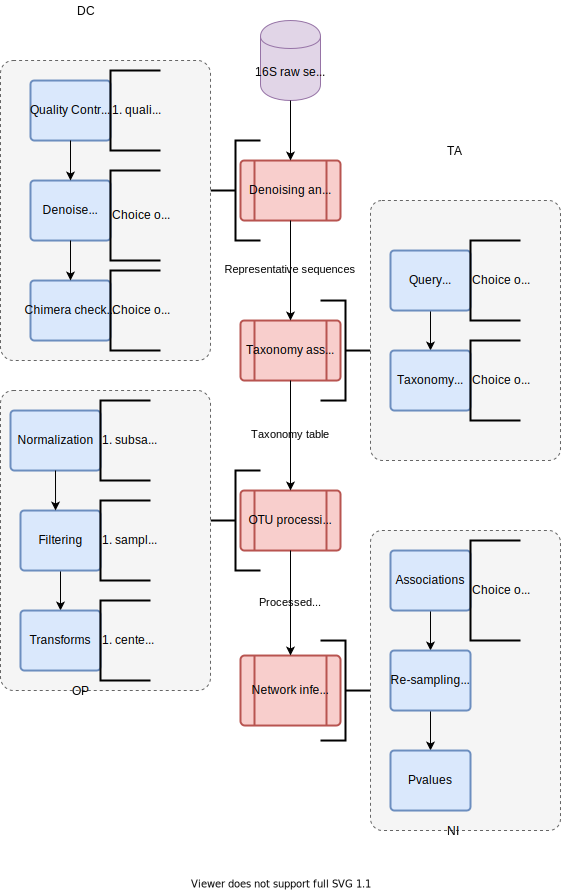
\includegraphics[width=0.67\linewidth]{figure1.pdf}
%DIFDELCMD <     %%%
\DIFdelendFL \DIFaddbeginFL 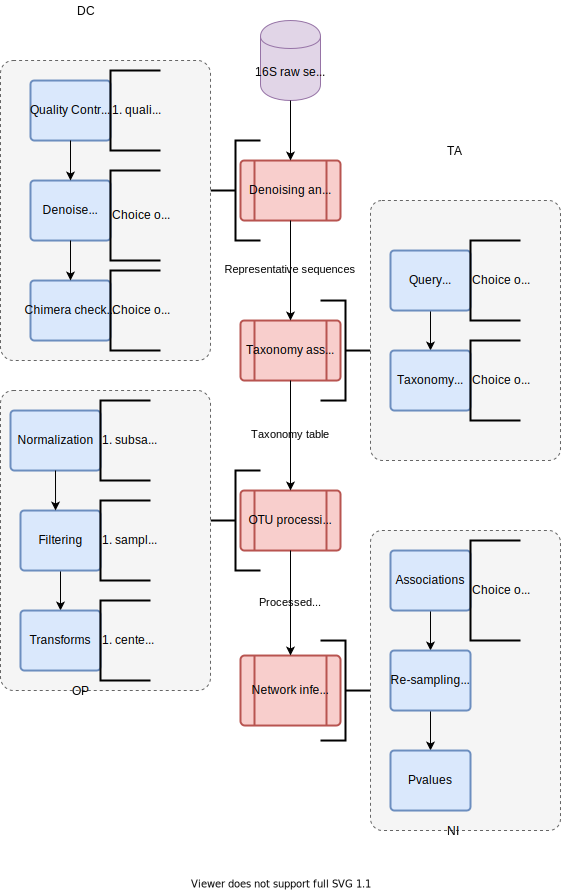
\includegraphics[width=0.74\linewidth]{figure1.pdf}
  \end{figure}
  \begin{figure}[H]
    \centering
    \DIFaddendFL \caption{
      \DIFdelbeginFL \textbf{\DIFdelFL{The workflow of the microbial co-occurrence analysis pipeline}}%DIFAUXCMD
\DIFdelendFL \DIFaddbeginFL \textbf{\DIFaddFL{The workflow of the }\ac{micone} \DIFaddFL{pipeline}}\DIFaddendFL .
      The steps \DIFaddbeginFL \DIFaddFL{of the workflow }\DIFaddendFL can be \DIFdelbeginFL \DIFdelFL{grouped }\DIFdelendFL \DIFaddbeginFL \DIFaddFL{broken down }\DIFaddendFL into \DIFdelbeginFL \DIFdelFL{four }\DIFdelendFL \DIFaddbeginFL \DIFaddFL{five }\DIFaddendFL major groups: \DIFaddbeginFL \textbf{\DIFaddFL{(SP)}} \textbf{\DIFaddFL{S}}\DIFaddFL{equence }\textbf{\DIFaddFL{P}}\DIFaddFL{rocessig, }\DIFaddendFL \textbf{(DC)} \textbf{D}enoising and \textbf{C}lustering, \textbf{(TA)} \textbf{T}axonomy \textbf{A}ssignment, \textbf{(OP)} \textbf{O}TU \DIFdelbeginFL \DIFdelFL{or }\DIFdelendFL \DIFaddbeginFL \DIFaddFL{and }\DIFaddendFL ESV \textbf{P}rocessing, and \textbf{(NI)} \textbf{N}etwork \textbf{I}nference.
      Each step incorporates several processes, each of which in turn have several alternate algorithms for the same task (indicated by the text to the right of the blue boxes).
      The text along the arrows describes the data that is being passed from one step to another.
      \DIFaddbeginFL \DIFaddFL{The final output of the pipeline is the consensus network generated from the inferred co-occurrence networks.
      }\DIFaddendFL For details on each process and \DIFaddbeginFL \DIFaddFL{the }\DIFaddendFL data \DIFdelbeginFL \DIFdelFL{types}\DIFdelendFL \DIFaddbeginFL \DIFaddFL{outputs}\DIFaddendFL , see Methods.
    }
    \label{fig:figure1}
  \end{figure}
\DIFaddbegin 



  \DIFaddend \FloatBarrier
  \newpage
  \DIFdelbegin %DIFDELCMD < 

%DIFDELCMD <   %%%
\DIFdelend \begin{figure}[H]
    \centering
    \DIFdelbeginFL %DIFDELCMD < 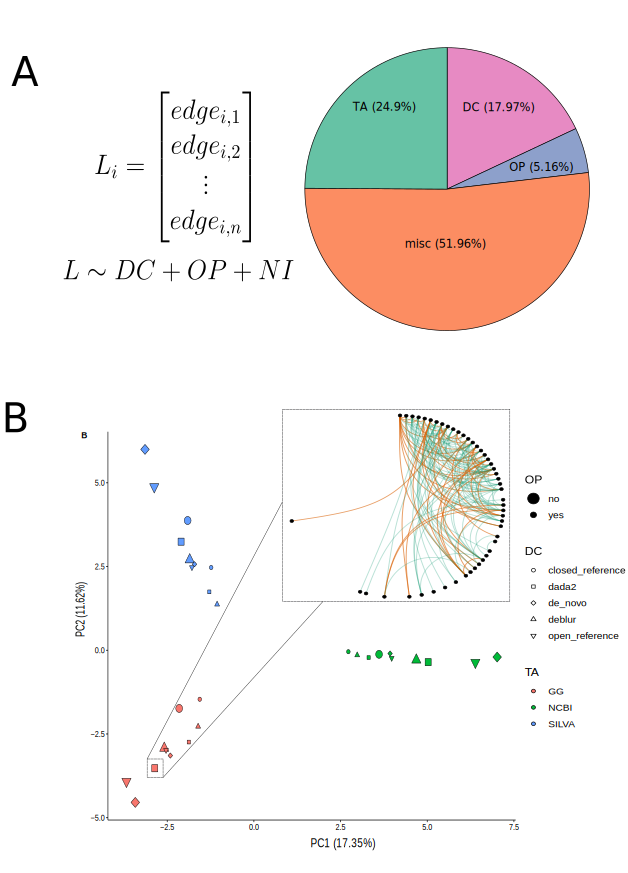
\includegraphics[width=0.85\linewidth]{figure2.pdf}
%DIFDELCMD <   %%%
\DIFdelendFL \DIFaddbeginFL 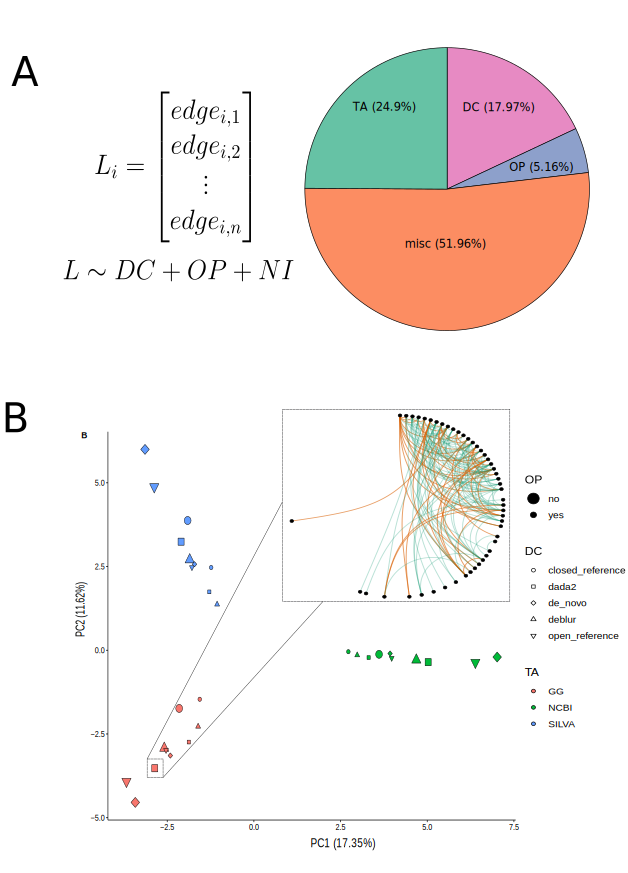
\includegraphics[width=\textwidth]{figure2.pdf}
  \DIFaddendFL \end{figure}
  \begin{figure}[H]
    \centering
    \caption{
      \DIFdelbeginFL \textbf{\DIFdelFL{The choice of database contributes to the most variance in the networks}}%DIFAUXCMD
\DIFdelFL{.
      }\DIFdelendFL \DIFaddbeginFL \textbf{\DIFaddFL{The representative sequences generated by the different denoising/clustering methods are very similar but differ in the sequences that are lower in abundance.}}
      \DIFaddendFL \textbf{(A)} The \DIFdelbeginFL \DIFdelFL{total relative variance in the networks contributed by the DC, TA and OP steps of the pipeline (right) and the linear model used to calculate the relative variance (left), see the Methods section for details.
      }\textbf{\DIFdelFL{(B)}} %DIFAUXCMD
\DIFdelFL{All combinations of inferred networks are shown as points on a PCA plot.
      The color of the points corresponds to the taxonomy database, the shape corresponds to the denoising/clustering method and the size corresponds to whether low abundance OTUs were removed or not.
      }\textbf{\DIFdelFL{(B inset)}} %DIFAUXCMD
\DIFdelFL{The network generated using DC=dada2, TA=GG, OP=no and NI=SPARCC and represents the particular point shown (big red square).
      The plot clearly shows that the points can be separated based on the TA step and that the differences due to the DC and OP steps are not as significant.
    }%DIFDELCMD < \MBLOCKRIGHTBRACE
%DIFDELCMD <     \label{fig:figure2}
%DIFDELCMD <   \end{figure}
%DIFDELCMD <   \FloatBarrier
%DIFDELCMD <   \newpage
%DIFDELCMD <   

%DIFDELCMD <   \begin{figure}
%DIFDELCMD <     \centering
%DIFDELCMD <     \includegraphics[width=\textwidth]{figure3.pdf}
%DIFDELCMD <     \caption{
%DIFDELCMD <       %%%
\textbf{\DIFdelFL{The representative sequences generated by the different denoising/clustering methods are very similar but differ in the sequences that are in low abundance.}}
      %DIFAUXCMD
\textbf{\DIFdelFL{(A)}} %DIFAUXCMD
\DIFdelFL{The }\DIFdelendFL average weighted UniFrac distance between the representative sequences shows that the representative sequences and their compositions are fairly identical between the methods \DIFdelbeginFL \DIFdelFL{,
      }\DIFdelendFL \DIFaddbeginFL \DIFaddFL{(with the exception of Deblur (DB)).
      }\DIFaddendFL \textbf{(B)} The relatively larger average unweighted UniFrac distance indicates that methods differ in their identification of sequences \DIFdelbeginFL \DIFdelFL{of low }\DIFdelendFL \DIFaddbeginFL \DIFaddFL{that are lower in }\DIFaddendFL abundance\DIFdelbeginFL \DIFdelFL{,
      }\DIFdelendFL \DIFaddbeginFL \DIFaddFL{.
      The number of }\ac{otu}\DIFaddFL{s or }\ac{esv}\DIFaddFL{s generated by the respective methods are provided in the parenthesis next to the names.
      The data used for the analysis in }\textbf{\DIFaddFL{(A, B)}} \DIFaddFL{were all the samples (healthy and autistic) from the fecal microbiome transplant dataset.
      }\DIFaddendFL \textbf{(C, D)} The distributions of the average weighted \DIFaddbeginFL \DIFaddFL{and unweighted }\DIFaddendFL UniFrac distance between the expected sequence profile and the \DIFdelbeginFL \DIFdelFL{calculated }\DIFdelendFL \DIFaddbeginFL \DIFaddFL{predicted }\DIFaddendFL sequence profile in \DIFaddbeginFL \DIFaddFL{the }\DIFaddendFL mock datasets.
      \DIFdelbeginFL \textbf{\DIFdelFL{(D)}} %DIFAUXCMD
\DIFdelendFL The distributions of the average \DIFdelbeginFL \DIFdelFL{unweighted }\DIFdelendFL \DIFaddbeginFL \DIFaddFL{weighted }\DIFaddendFL UniFrac distance show that \DIFdelbeginFL \DIFdelFL{dada2 }\DIFdelendFL \DIFaddbeginFL \DIFaddFL{de novo (DN) }\DIFaddendFL and \DIFdelbeginFL \DIFdelFL{Deblur }\DIFdelendFL \DIFaddbeginFL \DIFaddFL{open reference (OR) }\DIFaddendFL were the best performing methods in most of the datasets\DIFaddbeginFL \DIFaddFL{, while they are worst performing methods under the unweighted UniFrac metric}\DIFaddendFL .
      \DIFaddbeginFL \DIFaddFL{The good performance of dada2 (D2) under both distance metrics combined with its approach of identifying }\ac{esv}\DIFaddFL{s using de novo methods, prompts us to propose it as the default method for the DC step.
      The data used for the analysis in }\textbf{\DIFaddFL{(C, D)}} \DIFaddFL{were the mock datasets from mockrobiota~\mbox{%DIFAUXCMD
\cite{Bokulich2016}}\hskip0pt%DIFAUXCMD
.
    }\DIFaddendFL }
    \DIFdelbeginFL %DIFDELCMD < \label{fig:figure3}
%DIFDELCMD <   %%%
\DIFdelendFL \DIFaddbeginFL \label{fig:figure2}
  \DIFaddendFL \end{figure}
\DIFaddbegin 


  \DIFaddend \FloatBarrier
  \newpage
  \DIFdelbegin %DIFDELCMD < 

%DIFDELCMD <   %%%
\DIFdelend \begin{figure}[H]
    \centering
    \DIFdelbeginFL %DIFDELCMD < 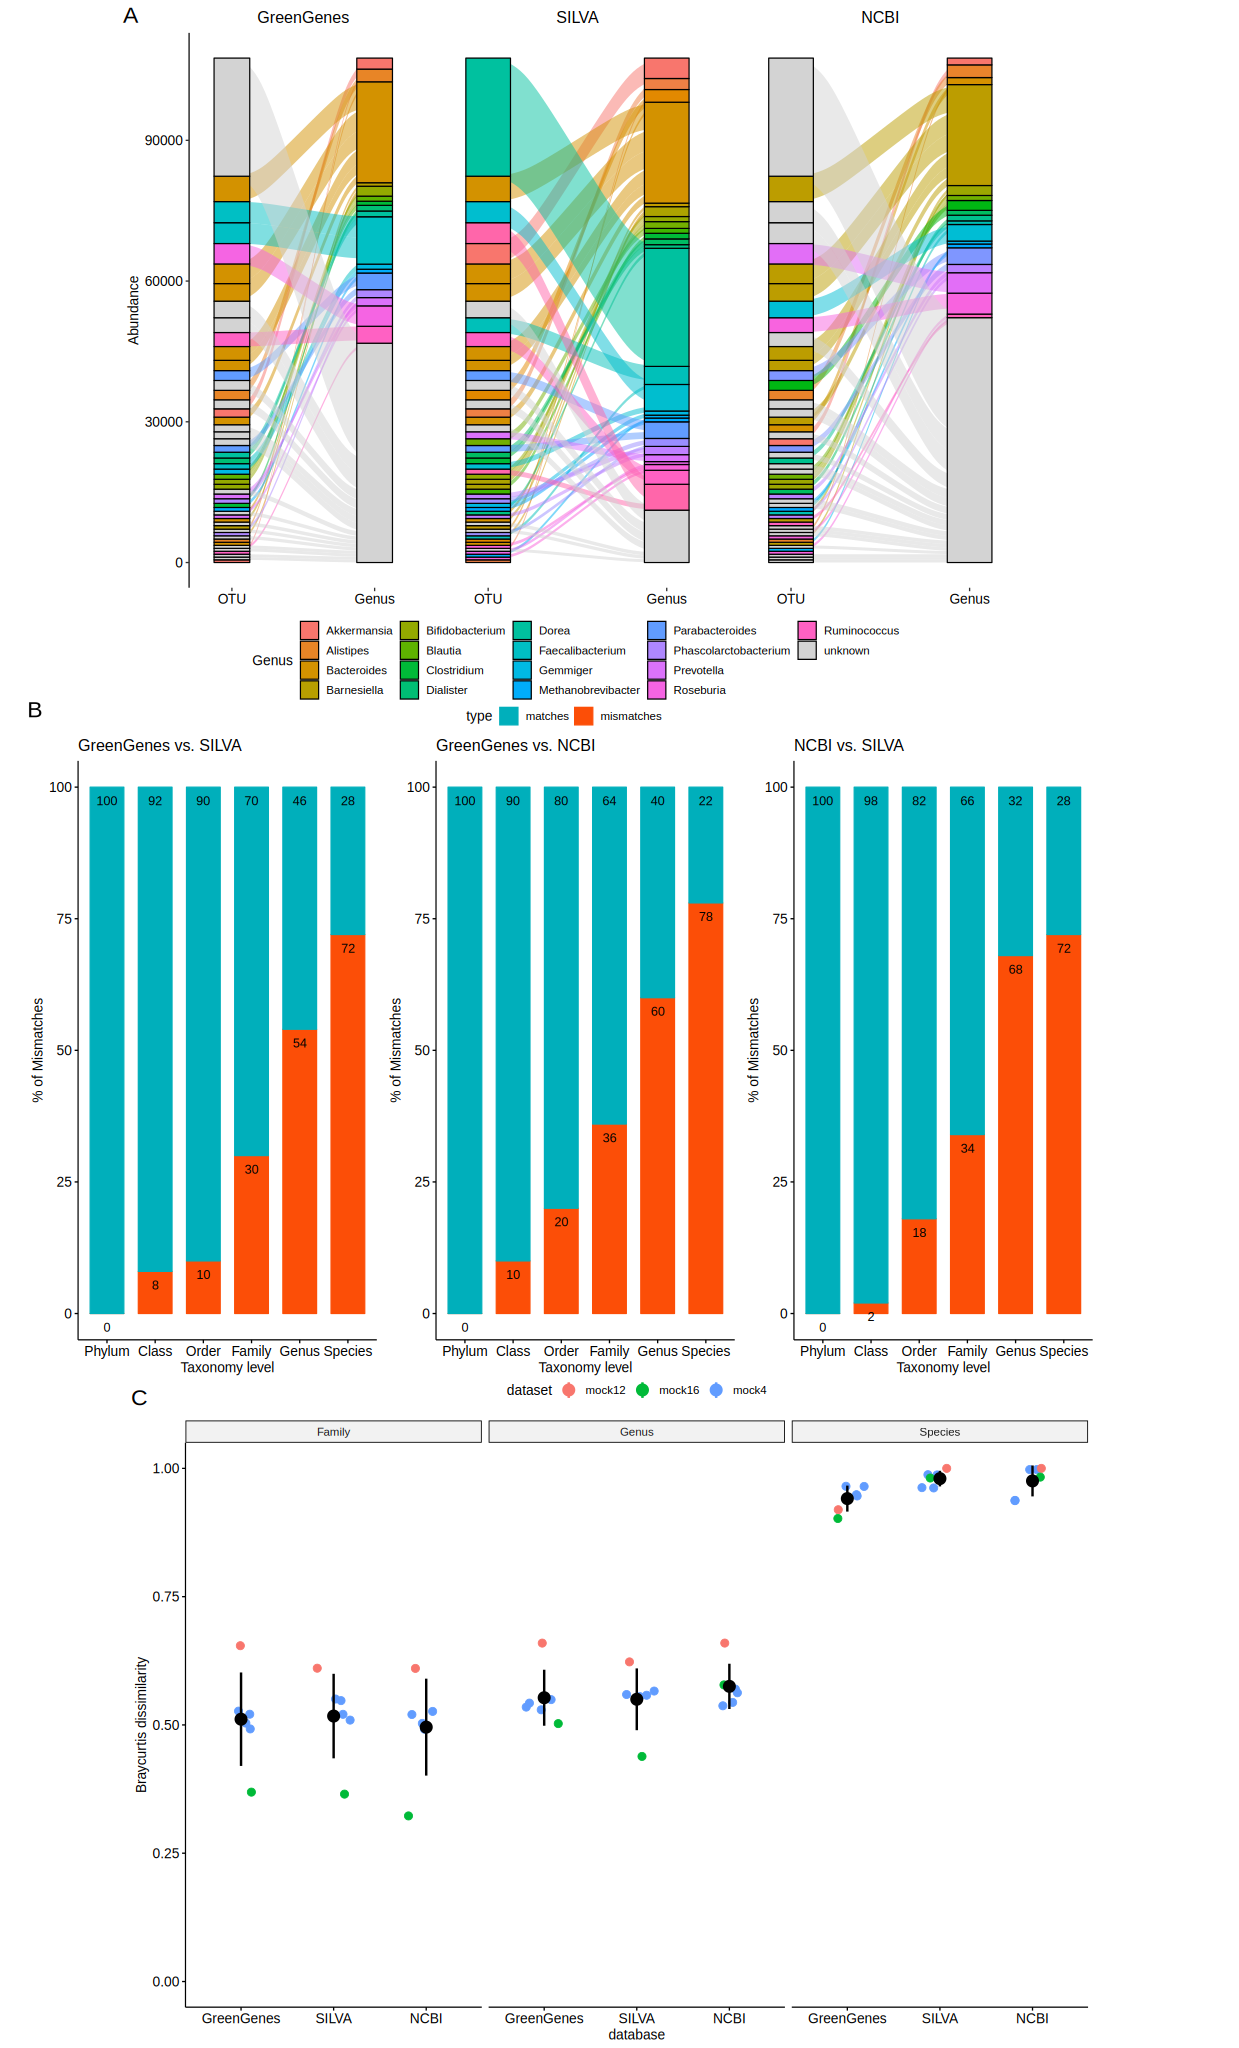
\includegraphics[width=0.9\textwidth,height=1.2\textwidth]{figure4.pdf}
%DIFDELCMD <   %%%
\DIFdelendFL \DIFaddbeginFL \includegraphics[width=\textwidth]{figure3.pdf}
  \DIFaddendFL \end{figure}
  \begin{figure}[H]
    \centering
    \caption{
      \DIFdelbeginFL \textbf{\DIFdelFL{Taxonomic reference databases vary widely in terms of their taxonomy assignments.}}
      %DIFAUXCMD
\DIFdelendFL \DIFaddbeginFL \textbf{\DIFaddFL{Taxonomic reference databases vary widely in terms of their taxonomy assignments beyond the Order level.}}
      \DIFaddendFL \textbf{(A)} The \DIFdelbeginFL \DIFdelFL{assignment }\DIFdelendFL \DIFaddbeginFL \DIFaddFL{assignments }\DIFaddendFL of the top 50 representative sequences to their respective taxonomies using the three different reference databases\DIFdelbeginFL \DIFdelFL{shows }\DIFdelendFL \DIFaddbeginFL \DIFaddFL{.
      This result illustrates }\DIFaddendFL how the same sequences are assigned to different Genus \DIFaddbeginFL \DIFaddFL{under the different databases}\DIFaddendFL .
      \DIFaddbeginFL \DIFaddFL{A significant portion of the representative sequences are assigned to an ``unknown'' Genus in two of three databases (}\ac{gg} \DIFaddFL{and }\ac{ncbi}\DIFaddFL{).
      }\DIFaddendFL \textbf{(B)} The \DIFdelbeginFL \DIFdelFL{percentage }\DIFdelendFL \DIFaddbeginFL \DIFaddFL{number }\DIFaddendFL of \DIFdelbeginFL %DIFDELCMD < \ac{otu}%%%
\DIFdelFL{s }\DIFdelendFL \DIFaddbeginFL \DIFaddFL{representative sequences }\DIFaddendFL assigned to the same taxonomic label when using different reference databases\DIFaddbeginFL \DIFaddFL{, shown for the top 100 sequences}\DIFaddendFL .
      The \DIFdelbeginFL \DIFdelFL{percentage }\DIFdelendFL \DIFaddbeginFL \DIFaddFL{number }\DIFaddendFL of mismatches \DIFdelbeginFL \DIFdelFL{decrease }\DIFdelendFL \DIFaddbeginFL \DIFaddFL{are fewer }\DIFaddendFL at higher taxonomic levels\DIFaddbeginFL \DIFaddFL{, }\DIFaddendFL but\DIFaddbeginFL \DIFaddFL{, }\DIFaddendFL even at the \DIFdelbeginFL \DIFdelFL{Phylum }\DIFdelendFL \DIFaddbeginFL \DIFaddFL{Order }\DIFaddendFL level there exists \DIFdelbeginFL \DIFdelFL{around 10}\DIFdelendFL \DIFaddbeginFL \DIFaddFL{greater than 51}\DIFaddendFL \% of mismatches\DIFaddbeginFL \DIFaddFL{, demonstrating the poor agreement in taxonomic labels assigned by the different databases}\DIFaddendFL .
      \DIFaddbeginFL \DIFaddFL{The data used for the analysis in }\textbf{\DIFaddFL{(A, B)}} \DIFaddFL{were all the samples (healthy and autistic) from the fecal microbiome transplant dataset.
      }\DIFaddendFL \textbf{(C)} The Bray-Curtis dissimilarity between the expected taxonomy profile and calculated taxonomy profile in the mock datasets shows that there is no singular best choice of database for every dataset\DIFaddbeginFL \DIFaddFL{, as all the databases have similar performance}\DIFaddendFL .
      \DIFaddbeginFL \DIFaddFL{However, we still recommend the }\ac{gg} \DIFaddFL{database and the Naive Bayes classifier as the defaults for the }\ac{micone} \DIFaddFL{pipeline.
      Due to the popularity of the }\ac{gg} \DIFaddFL{database, comparison against existing networks in literature will be easier since many published datasets make use of this database in their analyses.
      The datasets used for the analysis in }\textbf{\DIFaddFL{(C)}} \DIFaddFL{were the mock datasets from mockrobiota.
    }\DIFaddendFL }
    \DIFdelbeginFL %DIFDELCMD < \label{fig:figure4}
%DIFDELCMD <   %%%
\DIFdelendFL \DIFaddbeginFL \label{fig:figure3}
  \DIFaddendFL \end{figure}
\DIFaddbegin 


  \DIFaddend \FloatBarrier
  \newpage
  \DIFdelbegin %DIFDELCMD < 

%DIFDELCMD <   
%DIFDELCMD <   %%%
\DIFdelend \begin{figure}[H]
    \centering
    \DIFdelbeginFL %DIFDELCMD < 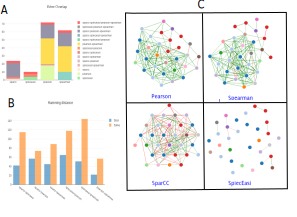
\includegraphics[width=0.9\textwidth]{figure5.pdf}
%DIFDELCMD <   %%%
\DIFdelendFL \DIFaddbeginFL 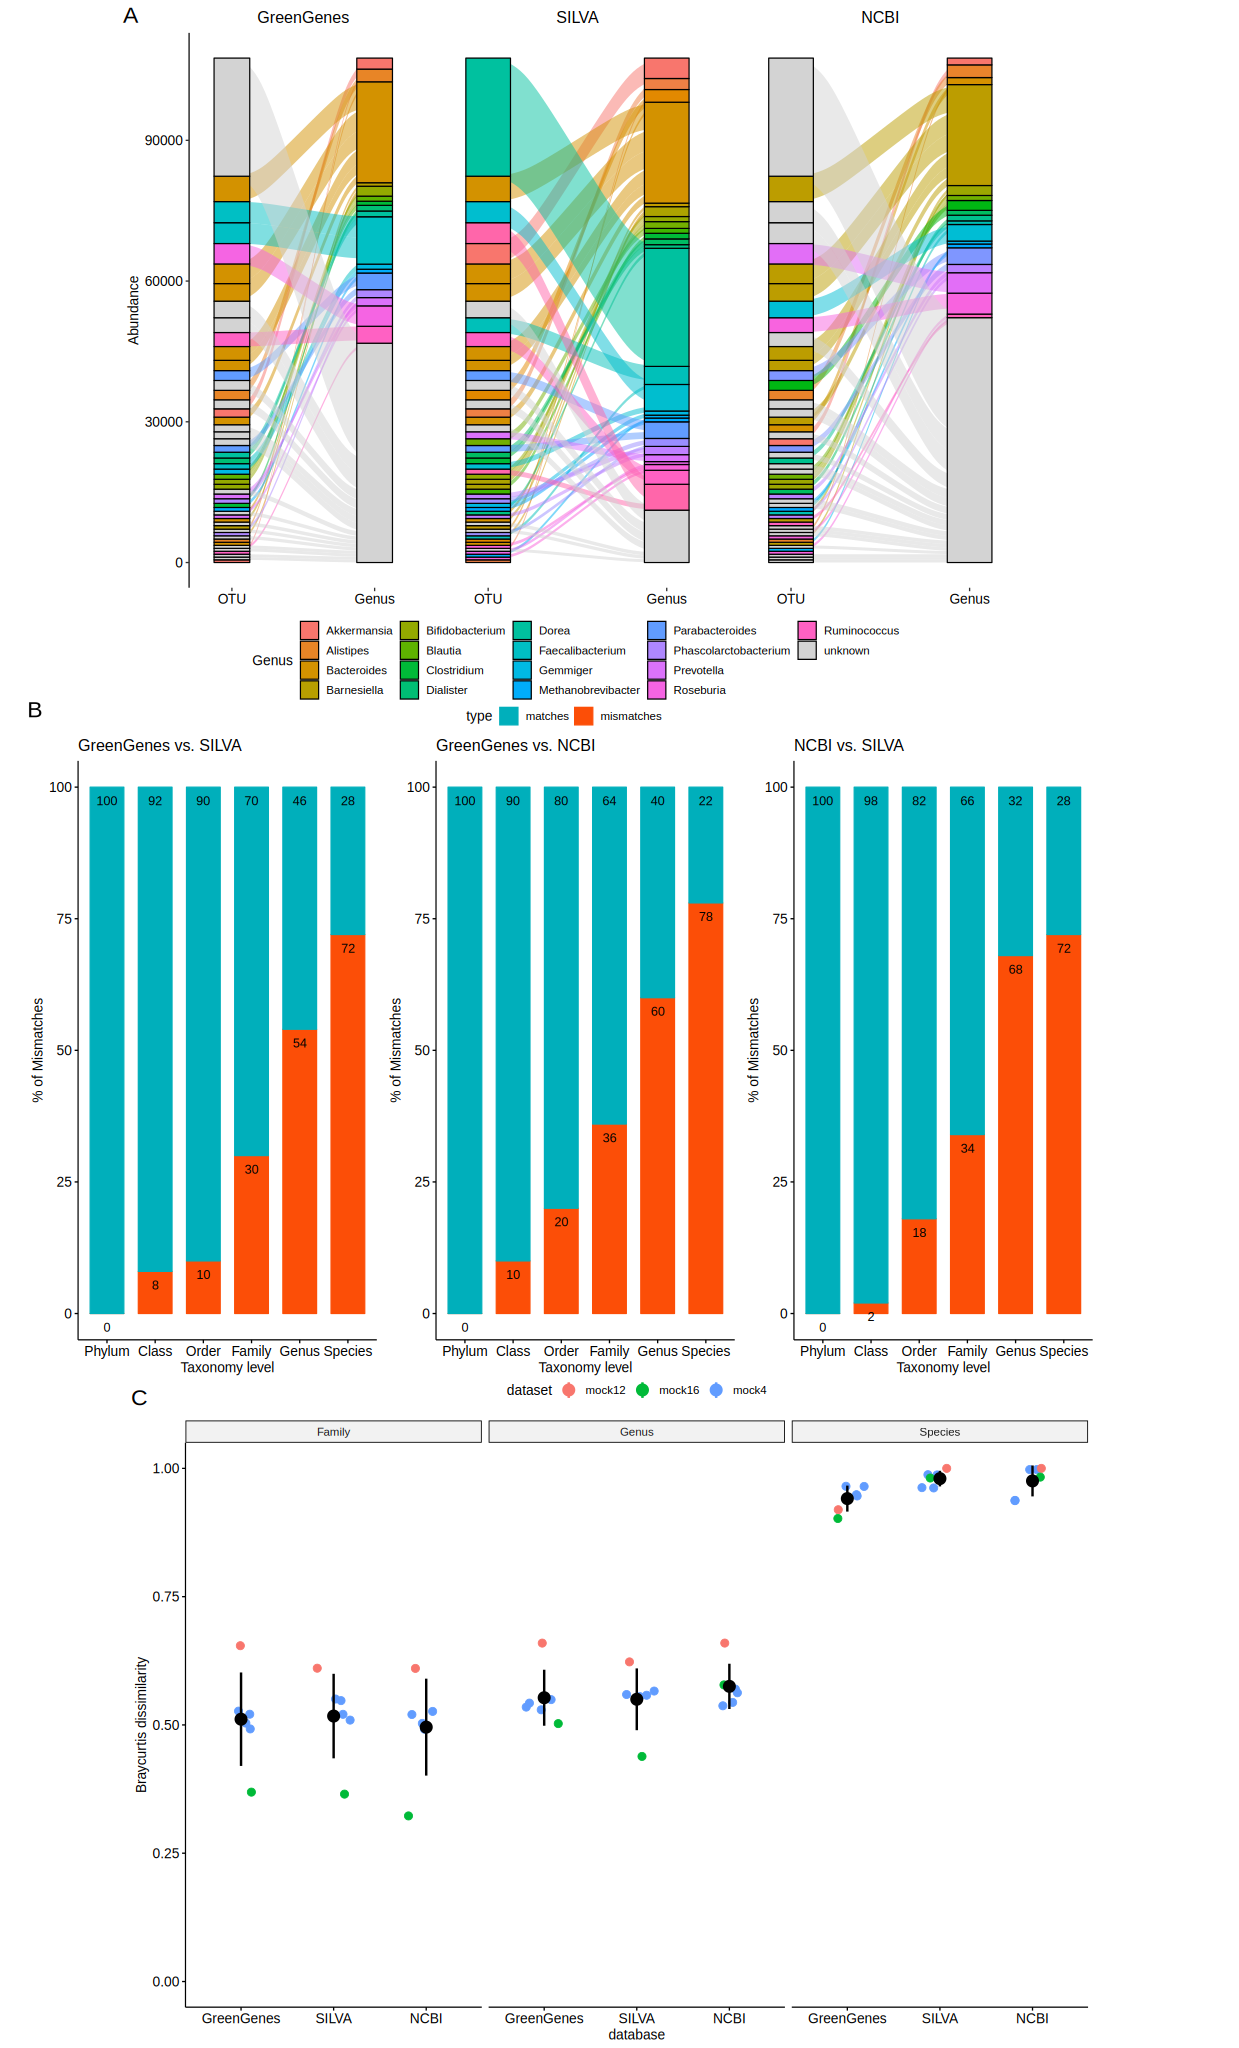
\includegraphics[width=\textwidth]{figure4.pdf}
  \DIFaddendFL \end{figure}
  \begin{figure}[H]
    \centering
    \caption{
      \textbf{Networks generated using different network inference methods show notable differences both in terms of edge-density and connectivity}.
      \textbf{(A)} The \DIFdelbeginFL \DIFdelFL{six }\DIFdelendFL \DIFaddbeginFL \DIFaddFL{nine }\DIFaddendFL different networks \DIFaddbeginFL \DIFaddFL{(excluding }\ac{mldm}\DIFaddFL{) }\DIFaddendFL generated by the different network inference methods are very dissimilar.
      The green links are positive associations and the orange links \DIFdelbeginFL \DIFdelFL{are }\DIFdelendFL \DIFaddbeginFL \DIFaddFL{represent }\DIFaddendFL negative associations.
      A threshold of 0.3 was set for the \DIFaddbeginFL \DIFaddFL{correlation-based }\DIFaddendFL methods \DIFdelbeginFL \DIFdelFL{that infer pairwise correlations }\DIFdelendFL (\ac{sparcc}, \DIFdelbeginFL \DIFdelFL{Spearman}\DIFdelendFL \DIFaddbeginFL \DIFaddFL{Propr}\DIFaddendFL , \DIFaddbeginFL \DIFaddFL{Spearman and }\DIFaddendFL Pearson) and \DIFdelbeginFL \DIFdelFL{no }\DIFdelendFL \DIFaddbeginFL \DIFaddFL{a }\DIFaddendFL threshold \DIFaddbeginFL \DIFaddFL{of 0.01 }\DIFaddendFL was set for the other \DIFaddbeginFL \DIFaddFL{direct association }\DIFaddendFL methods.
      \DIFaddbeginFL \DIFaddFL{The correlation-based methods in general produce graph with higher edge-densities.
      }\DIFaddendFL \textbf{(B)} The node overlap Upset plot \DIFdelbeginFL \DIFdelFL{~\mbox{%DIFAUXCMD
\cite{Lex} }\hskip0pt%DIFAUXCMD
}\DIFdelendFL indicates that all the networks have a large \DIFdelbeginFL \DIFdelFL{number }\DIFdelendFL \DIFaddbeginFL \DIFaddFL{proportion }\DIFaddendFL of common nodes involved in connections \DIFaddbeginFL \DIFaddFL{(33 out of 68)}\DIFaddendFL .
      Whereas, \textbf{(C)} \DIFdelbeginFL \DIFdelFL{The }\DIFdelendFL \DIFaddbeginFL \DIFaddFL{the }\DIFaddendFL edge overlap Upset plot shows that a very small fraction of these connections are actually shared \DIFaddbeginFL \DIFaddFL{(8 out of 202)}\DIFaddendFL .
      \DIFaddbeginFL \DIFaddFL{The data used in this analysis were the healthy stool samples from the fecal microbiome transplant dataset.
      }\ac{mldm} \DIFaddFL{is not shown in the comparisons because the algorithm failed to converge for most of the network combinations.
    }\DIFaddendFL }
    \DIFaddbeginFL \label{fig:figure4}
  \end{figure}


  \FloatBarrier
  \newpage
  \begin{figure}[H]
    \centering
    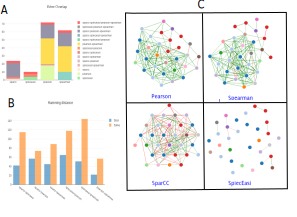
\includegraphics[width=1.0\linewidth]{figure5.pdf}
  \end{figure}
  \begin{figure}[H]
    \centering
    \caption{
      \textbf{\DIFaddFL{The precision and sensitivity of the inferred networks on the NorTA synthetic interaction data.}}
      \DIFaddFL{The ``I'' prefix indicates the individual network inference methods and the ``X'' prefix denotes the consensus based methods that are a part of }\ac{micone}\DIFaddFL{.
      The different consensus based methods used are: pvalue merging (PM), scaled-sum (SS) and simple voting (SV) method.
      Pearson and Spearman methods are not used in the calculation of the consensus.
      Among all the independent network inference methods, }\ac{spieceasi} \DIFaddFL{has the best average precision (0.944), but the overall best precision was consistently obtained by the scaled-sum method (0.956, 0.985 and 1.000).
      The simple voting method when using presence of edges in all inferred networks as a requirement (parameter value 1.000), also outperforms }\ac{spieceasi} \DIFaddFL{on average precision (0.969).
      Although }\ac{spieceasi} \DIFaddFL{has a higher performance on sensitivity, if the goal of network inference is to obtain the list of associations that have a high probability of existing in the real microbial community, then the consensus methods perform better.
      Therefore, we recommend the scaled-sum consensus method as the default tool for network inference.
    }}
    \DIFaddendFL \label{fig:figure5}
  \end{figure}
\DIFaddbegin 


  \DIFaddend \FloatBarrier
  \newpage
  %DIF >  TODO: Add equations for the linear model to the left of the pie chart
  \DIFaddbegin \begin{figure}[H]
    \centering
    \includegraphics[width=\textwidth]{figure6.pdf}
  \end{figure}
  \begin{figure}[H]
    \centering
      \caption{
      \textbf{\DIFaddFL{The choice of reference database contributes to the most variance in the networks}}\DIFaddFL{.
      }\textbf{\DIFaddFL{(A)}} \DIFaddFL{The percentage of variance in the networks contributed by the DC, CC (chimera checking), TA and OP steps of the pipeline (right) and the linear model used to calculate the variance (left), see the Methods section for details.
      The data used for the analysis were the healthy stool samples from the fecal microbiome transplant dataset~\mbox{%DIFAUXCMD
\cite{Kang2017}}\hskip0pt%DIFAUXCMD
.
      The taxonomy database contributes most to the variance between the networks (65.4\%) followed by the filtering of the counts matrix (26.8\%) in the OP step.
      The variation due to the DC and CC steps are comparatively not as significant.
      }\textbf{\DIFaddFL{(B)}} \DIFaddFL{All combinations of inferred networks are shown as points on a PCA plot.
      Each point on the PCA plot represents a network inferred using different combinations of tools and parameters that are available in the }\ac{micone} \DIFaddFL{pipeline.
      The color of the points corresponds to the reference taxonomy database used to reconstruct those networks (left), and the network inference algorithm used to infer the networks (right).
      The points on the PCA plot can be grouped based on the TA step, but at the NI step only some methods create high variability in the inferred networks.
    }}
    \label{fig:figure6}
  \end{figure}
\DIFaddend 


  \DIFdelbegin %DIFDELCMD < \begin{figure}[h]
%DIFDELCMD <     %%%
\DIFdelendFL \DIFaddbeginFL \FloatBarrier
  \newpage
  %DIF >  TODO: Verify the validity of Figure 7A and 7B again
  %DIF >  Are they both using consensus?
  \begin{figure}[H]
    \DIFaddendFL \centering
    \DIFdelbeginFL %DIFDELCMD < \includegraphics[width=0.85\linewidth]{figure6.pdf}
%DIFDELCMD <     %%%
\DIFdelendFL \DIFaddbeginFL 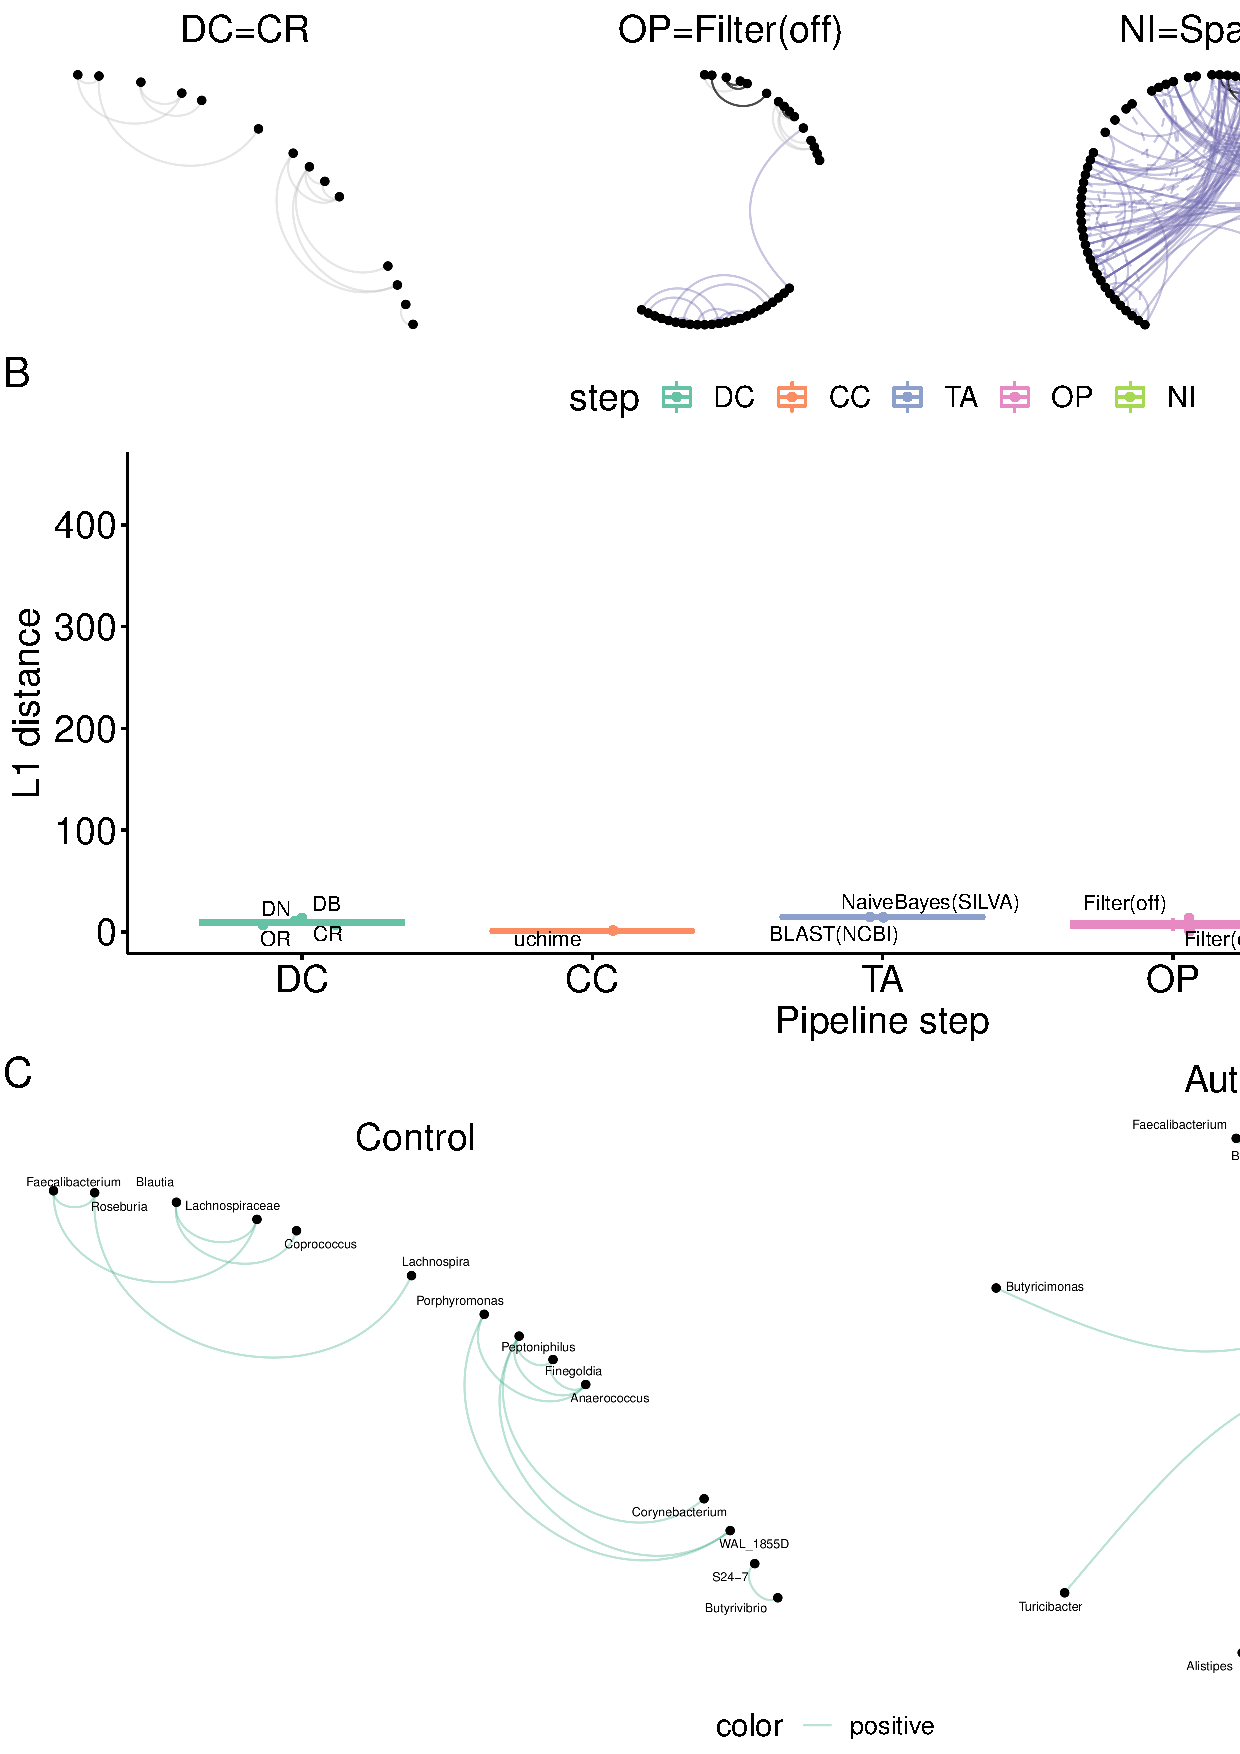
\includegraphics[width=1.0\linewidth]{figure7.pdf}
  \end{figure}
  \begin{figure}[H]
    \centering
    \DIFaddendFL \caption{
      \DIFdelbeginFL \textbf{\DIFdelFL{Network inference and taxonomic assignment have the highest influence on the inferred network structures.}}
      %DIFAUXCMD
\DIFdelendFL \DIFaddbeginFL \textbf{\DIFaddFL{The consensus algorithm drastically reduces variability in the networks due to upstream data processing methods and increases robustness of inferred networks}}
      \DIFaddendFL \textbf{(A)} The network constructed using the default pipeline parameters (DC=\ac{dada2}, \DIFaddbeginFL \DIFaddFL{CC=remove bimera, }\DIFaddendFL TA=\DIFdelbeginFL %DIFDELCMD < \ac{ncbi}%%%
\DIFdelendFL \DIFaddbeginFL \ac{gg}\DIFaddendFL , OP=\DIFaddbeginFL \DIFaddFL{Filter(}\DIFaddendFL on\DIFaddbeginFL \DIFaddFL{)}\DIFaddendFL , NI=\DIFdelbeginFL %DIFDELCMD < \ac{sparcc}%%%
\DIFdelendFL \DIFaddbeginFL \DIFaddFL{scaled-sum consensus}\DIFaddendFL ) is compared with networks generated when one of the steps use a different tool.
      The common connections (common with the default network) are in black, connections unique to the network are colored purple and connections in the default network\DIFaddbeginFL \DIFaddFL{, }\DIFaddendFL but not present in the current network are gray.
      \DIFaddbeginFL \DIFaddFL{Changing the NI, TA and OP steps leads to the creation of the most number of new nodes and edges.
      }\DIFaddendFL \textbf{(B)} The \DIFaddbeginFL \DIFaddFL{boxplot showing the }\DIFaddendFL L1 distance between the \DIFaddbeginFL \DIFaddFL{default network and the }\DIFaddendFL networks generated by changing one step of the default pipeline\DIFdelbeginFL \DIFdelFL{and }\DIFdelendFL \DIFaddbeginFL \DIFaddFL{.
      The high value of L1 distances for }\DIFaddendFL the network \DIFdelbeginFL \DIFdelFL{generated using }\DIFdelendFL \DIFaddbeginFL \DIFaddFL{inference step as compared to }\DIFaddendFL the \DIFdelbeginFL \DIFdelFL{default parameters.
    }%DIFDELCMD < \MBLOCKRIGHTBRACE
%DIFDELCMD <     \label{fig:figure6}
%DIFDELCMD <   \end{figure}
%DIFDELCMD <   \FloatBarrier
%DIFDELCMD <   \newpage
%DIFDELCMD < 

%DIFDELCMD <   \begin{figure}[h]
%DIFDELCMD <     \centering
%DIFDELCMD <     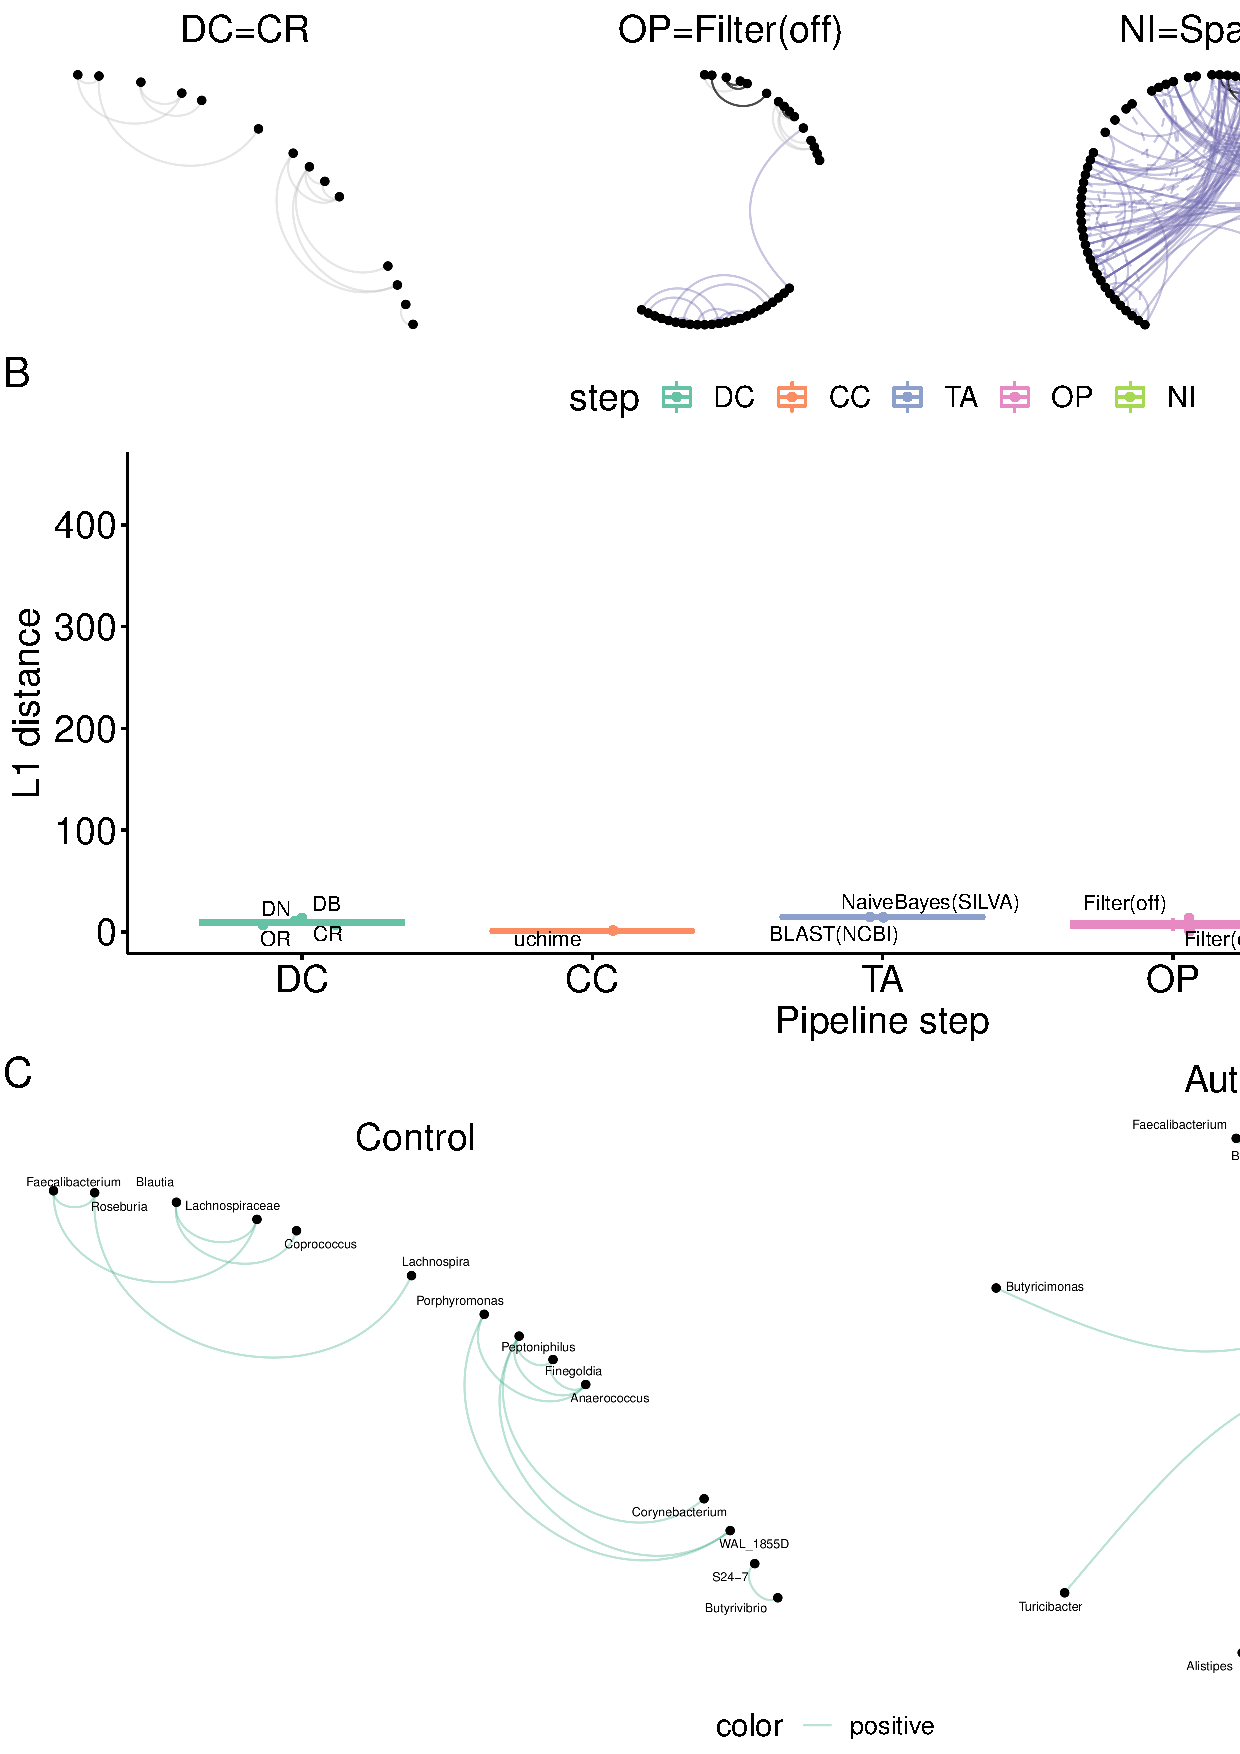
\includegraphics[width=17cm]{figure7.pdf}
%DIFDELCMD <     \caption{
%DIFDELCMD <       %%%
\DIFdelFL{The }\DIFdelendFL \DIFaddbeginFL \DIFaddFL{other steps demonstrates how the }\DIFaddendFL consensus \DIFaddbeginFL \DIFaddFL{method is able to reduce the variability in the }\DIFaddendFL networks \DIFdelbeginFL \DIFdelFL{generated using }\DIFdelendFL \DIFaddbeginFL \DIFaddFL{in }\DIFaddendFL the \DIFdelbeginFL \DIFdelFL{default }\DIFdelendFL \DIFaddbeginFL \DIFaddFL{other steps of the }\DIFaddendFL pipeline\DIFdelbeginFL \DIFdelFL{settings}\DIFdelendFL .
      \DIFdelbeginFL \textbf{\DIFdelFL{(A)}} %DIFAUXCMD
\DIFdelFL{Co-occurrence network of }\DIFdelendFL \DIFaddbeginFL \DIFaddFL{This also shows that even though many new nodes were added in (A) when }\DIFaddendFL the \DIFdelbeginFL \DIFdelFL{Hard Palate microbiome }\DIFdelendFL \DIFaddbeginFL \DIFaddFL{TA and OP steps were changed, the L1 distances remain fairly small.
      }\textbf{\DIFaddFL{(C)}} \DIFaddFL{The networks }\DIFaddendFL generated \DIFdelbeginFL \DIFdelFL{from }\DIFdelendFL \DIFaddbeginFL \DIFaddFL{for the control (left) and autistic (right) }\DIFaddendFL samples \DIFdelbeginFL \DIFdelFL{of healthy subjects }\DIFdelendFL in \DIFdelbeginFL \DIFdelFL{a periodontal diseases study.
      }\textbf{\DIFdelFL{(B)}} %DIFAUXCMD
\DIFdelFL{Co-occurrence network of }\DIFdelendFL the \DIFdelbeginFL \DIFdelFL{Stool }\DIFdelendFL \DIFaddbeginFL \DIFaddFL{fecal }\DIFaddendFL microbiome \DIFaddbeginFL \DIFaddFL{transplant dataset.
      These networks were }\DIFaddendFL generated \DIFdelbeginFL \DIFdelFL{from samples of healthy subjects }\DIFdelendFL \DIFaddbeginFL \DIFaddFL{using the default tools and parameters recommended by the }\ac{micone} \DIFaddFL{pipeline.
      The data used }\DIFaddendFL in \DIFdelbeginFL \DIFdelFL{a }\DIFdelendFL \DIFaddbeginFL \DIFaddFL{this analysis were the healthy stool samples from the }\DIFaddendFL fecal microbiome transplant \DIFdelbeginFL \DIFdelFL{study}\DIFdelendFL \DIFaddbeginFL \DIFaddFL{dataset}\DIFaddendFL .
    }
    \label{fig:figure7}
  \end{figure}
\DIFaddbegin 



\DIFaddend %!TEX root = ../main.tex

\newpage
\section*{Supplementary}

  \DIFaddbegin {\color{red} \DIFadd{Tables S1-S5 will be moved to GitHub}}

  \DIFaddend \renewcommand{\thefigure}{S\arabic{figure}}
  \setcounter{figure}{0}

  \renewcommand{\thetable}{S\arabic{table}}
  \setcounter{table}{0}

  \DIFdelbegin %DIFDELCMD < \begin{table}[h]
%DIFDELCMD < \resizebox{\textwidth}{!}{
%DIFDELCMD < \begin{tabular}{lllll}
%DIFDELCMD < \hline
%DIFDELCMD < \textbf{Step}                             & \textbf{Task}                                            & \textbf{Tool}                          & \textbf{Parameter}                     & \textbf{Value}                                                                                           \\ \hline
%DIFDELCMD < \multirow{29}{*}{Denosing and Clustering} & \multicolumn{1}{c}{\multirow{9}{*}{Sequence Processing}} & \multirow{2}{*}{join\_reads}           & min\_overlap                           & 6                                                                                                        \\
%DIFDELCMD <                                           & \multicolumn{1}{c}{}                                     &                                        & perc\_max\_diff                        & 8                                                                                                        \\
%DIFDELCMD <                                           & \multicolumn{1}{c}{}                                     & \multirow{2}{*}{demultiplex\_illumina} & rev\_comp\_barcodes                    & False                                                                                                    \\
%DIFDELCMD <                                           & \multicolumn{1}{c}{}                                     &                                        & rev\_comp\_mapping\_barcodes           & False                                                                                                    \\
%DIFDELCMD <                                           & \multicolumn{1}{c}{}                                     & demultiplex\_454                       & -                                      & -                                                                                                        \\
%DIFDELCMD <                                           & \multicolumn{1}{c}{}                                     & \multirow{4}{*}{trim\_filter\_fixed}   & seq\_sample\_size                      & 10,000                                                                                                   \\
%DIFDELCMD <                                           & \multicolumn{1}{c}{}                                     &                                        & ncpus                                  & 1                                                                                                        \\
%DIFDELCMD <                                           & \multicolumn{1}{c}{}                                     &                                        & trunc\_q                               & 2                                                                                                        \\
%DIFDELCMD <                                           & \multicolumn{1}{c}{}                                     &                                        & max\_ee                                & 2                                                                                                        \\ \cline{2-5}
%DIFDELCMD <                                           & \multirow{3}{*}{Chimera Checking}                        & uchime                                 & -                                      & -                                                                                                        \\
%DIFDELCMD <                                           &                                                          & \multirow{2}{*}{remove\_bimera}        & ncpus                                  & 1                                                                                                        \\
%DIFDELCMD <                                           &                                                          &                                        & chimera\_method                        & consensus                                                                                                \\ \cline{2-5}
%DIFDELCMD <                                           & \multirow{17}{*}{Denoise Cluster}                        & \multirow{3}{*}{de\_novo}              & enable\_rev\_strand\_match             & True                                                                                                     \\
%DIFDELCMD <                                           &                                                          &                                        & suppress\_de\_novo\_chimera\_detection & True                                                                                                     \\
%DIFDELCMD <                                           &                                                          &                                        & ncpus                                  & 1                                                                                                        \\
%DIFDELCMD <                                           &                                                          & \multirow{4}{*}{closed\_reference}     & enable\_rev\_strand\_match             & True                                                                                                     \\
%DIFDELCMD <                                           &                                                          &                                        & suppress\_de\_novo\_chimera\_detection & True                                                                                                     \\
%DIFDELCMD <                                           &                                                          &                                        & ncpus                                  & 1                                                                                                        \\
%DIFDELCMD <                                           &                                                          &                                        & reference\_sequences                   & 97\_otus.fasta                                                                                           \\
%DIFDELCMD <                                           &                                                          & \multirow{5}{*}{open\_reference}       & enable\_rev\_strand\_match             & True                                                                                                     \\
%DIFDELCMD <                                           &                                                          &                                        & suppress\_de\_novo\_chimera\_detection & True                                                                                                     \\
%DIFDELCMD <                                           &                                                          &                                        & ncpus                                  & 1                                                                                                        \\
%DIFDELCMD <                                           &                                                          &                                        & reference\_sequences                   & 97\_otus.fasta                                                                                           \\
%DIFDELCMD <                                           &                                                          &                                        & picking\_method                        & uclust                                                                                                   \\
%DIFDELCMD <                                           &                                                          & \multirow{2}{*}{dada2}                 & ncpus                                  & 1                                                                                                        \\
%DIFDELCMD <                                           &                                                          &                                        & big\_data                              & FALSE                                                                                                    \\
%DIFDELCMD <                                           &                                                          & \multirow{3}{*}{deblur}                & ncpus                                  & 1                                                                                                        \\
%DIFDELCMD <                                           &                                                          &                                        & mind\_reads                            & 2                                                                                                        \\
%DIFDELCMD <                                           &                                                          &                                        & min\_size                              & 2                                                                                                        \\ \hline
%DIFDELCMD < \multirow{7}{*}{Taxonomy Assignment}      & \multirow{7}{*}{Assign}                                  & \multirow{3}{*}{naive\_bayes}          & confidence                             & 0.7                                                                                                      \\
%DIFDELCMD <                                           &                                                          &                                        & mem\_per\_core                         & 8G                                                                                                       \\
%DIFDELCMD <                                           &                                                          &                                        & ncpus                                  & 1                                                                                                        \\
%DIFDELCMD <                                           &                                                          & \multirow{4}{*}{blast}                 & max\_accepts                           & 10                                                                                                       \\
%DIFDELCMD <                                           &                                                          &                                        & perc\_identity                         & 0.8                                                                                                      \\
%DIFDELCMD <                                           &                                                          &                                        & evalue                                 & 0.001                                                                                                    \\
%DIFDELCMD <                                           &                                                          &                                        & min\_consensus                         & 0.51                                                                                                     \\ \hline
%DIFDELCMD < \multirow{12}{*}{OTU/ESV Processing}      & \multirow{5}{*}{Filter}                                  & \multirow{3}{*}{abundance}             & count\_thres                           & 500                                                                                                      \\
%DIFDELCMD <                                           &                                                          &                                        & prevalence\_thres                      & 0.05                                                                                                     \\
%DIFDELCMD <                                           &                                                          &                                        & abundance\_thres                       & 0.01                                                                                                     \\
%DIFDELCMD <                                           &                                                          & group                                  & tax\_levels                            & \begin{tabular}[c]{@{}l@{}}{[}'Phylum', 'Class', 'Order',\\ 'Family', 'Genus', 'Species'{]}\end{tabular} \\
%DIFDELCMD <                                           &                                                          & partition                              & -                                      & -                                                                                                        \\ \cline{2-5}
%DIFDELCMD <                                           & \multirow{6}{*}{Transform}                               & \multirow{6}{*}{normalize}             & count\_thres                           & 500                                                                                                      \\
%DIFDELCMD <                                           &                                                          &                                        & axis                                   & sample                                                                                                   \\
%DIFDELCMD <                                           &                                                          &                                        & prevalence\_thres                      & 0.05                                                                                                     \\
%DIFDELCMD <                                           &                                                          &                                        & abundace\_thres                        & 0.01                                                                                                     \\
%DIFDELCMD <                                           &                                                          &                                        & rm\_sparse\_obs                        & True                                                                                                     \\
%DIFDELCMD <                                           &                                                          &                                        & rm\_sparse\_samples                    & True                                                                                                     \\ \cline{2-5}
%DIFDELCMD <                                           & Export                                                   & biom2tsv                               & -                                      & -                                                                                                        \\ \hline
%DIFDELCMD < \multirow{17}{*}{Network Inference}       & \multirow{4}{*}{Bootstrap}                               & \multirow{3}{*}{resample}              & bootstraps                             & 1000                                                                                                     \\
%DIFDELCMD <                                           &                                                          &                                        & ncpus                                  & 1                                                                                                        \\
%DIFDELCMD <                                           &                                                          &                                        & filter\_flag                           & True                                                                                                     \\
%DIFDELCMD <                                           &                                                          & pvalue                                 & ncpus                                  & 1                                                                                                        \\ \cline{2-5}
%DIFDELCMD <                                           & \multirow{12}{*}{Correlation}                            & \multirow{2}{*}{sparcc}                & iterations                             & 50                                                                                                       \\
%DIFDELCMD <                                           &                                                          &                                        & ncpus                                  & 1                                                                                                        \\
%DIFDELCMD <                                           &                                                          & pearson                                & -                                      & -                                                                                                        \\
%DIFDELCMD <                                           &                                                          & spearman                               & -                                      & -                                                                                                        \\
%DIFDELCMD <                                           &                                                          & \multirow{5}{*}{spieceasi}             & method                                 & mb                                                                                                       \\
%DIFDELCMD <                                           &                                                          &                                        & ncpus                                  & 1                                                                                                        \\
%DIFDELCMD <                                           &                                                          &                                        & nreps                                  & 50                                                                                                       \\
%DIFDELCMD <                                           &                                                          &                                        & nlambda                                & 20                                                                                                       \\
%DIFDELCMD <                                           &                                                          &                                        & lambda\_min\_ratio                     & 1e-2                                                                                                     \\
%DIFDELCMD <                                           &                                                          & \multirow{2}{*}{mldm}                  & z\_mean                                & 1                                                                                                        \\
%DIFDELCMD <                                           &                                                          &                                        & max\_iteration                         & 1500                                                                                                     \\
%DIFDELCMD <                                           &                                                          & magma                                  & -                                      & -                                                                                                        \\ \cline{2-5}
%DIFDELCMD <                                           & Network                                                  & make\_network                          & -                                      & -                                                                                                        \\ \hline
%DIFDELCMD < \end{tabular}
%DIFDELCMD < }
%DIFDELCMD < %%%
\DIFdelendFL %DIF >  TODO: Convert to booktabs style?
\DIFaddbeginFL \begin{table}[H]
\centering
\small
\begin{tabular}{|c|c|c|c|}
\hline
 \textbf{\DIFaddFL{Task}}                   & \textbf{\DIFaddFL{Module}}                                   & \textbf{\DIFaddFL{Parameter}}           & \textbf{\DIFaddFL{Value}}   \\ \hline
 \multirow{6}{*}{Demultiplexing} & \multirow{3}{*}{demultiplexing\_illumina\_single} & \DIFaddFL{barcode\_column              }& \DIFaddFL{barcode-sequence }\\
                                 &                                                   & \DIFaddFL{rev\_comp\_barcodes          }& \DIFaddFL{false            }\\
                                 &                                                   & \DIFaddFL{rev\_comp\_mapping\_barcodes }& \DIFaddFL{false            }\\ \cline{3-4}
                                 & \multirow{3}{*}{demultiplexing\_illumina\_paired} & \DIFaddFL{barcode\_column              }& \DIFaddFL{barcode-sequence }\\
                                 &                                                   & \DIFaddFL{rev\_comp\_barcodes          }& \DIFaddFL{false            }\\
                                 &                                                   & \DIFaddFL{rev\_comp\_mapping\_barcodes }& \DIFaddFL{false            }\\ \cline{2-4}
 \multirow{8}{*}{Trimming}       & \DIFaddFL{export\_visualization\_single                     }& \DIFaddFL{seq\_samplesize              }& \DIFaddFL{10000            }\\ \cline{3-4}
                                 & \DIFaddFL{export\_visualization\_paired                     }& \DIFaddFL{seq\_samplesize              }& \DIFaddFL{10000            }\\ \cline{3-4}
                                 & \multirow{3}{*}{trimming\_single}                 & \DIFaddFL{ncpus                        }& \DIFaddFL{1                }\\
                                 &                                                   & \DIFaddFL{max\_ee                      }& \DIFaddFL{2                }\\
                                 &                                                   & \DIFaddFL{trunc\_q                     }& \DIFaddFL{2                }\\ \cline{3-4}
                                 & \multirow{3}{*}{trimming\_paired}                 & \DIFaddFL{ncpus                        }& \DIFaddFL{1                }\\
                                 &                                                   & \DIFaddFL{max\_ee                      }& \DIFaddFL{2                }\\
                                 &                                                   & \DIFaddFL{trunc\_q                     }& \DIFaddFL{2                }\\ \hline
\end{tabular}
\DIFaddendFL \caption{The default parameters used in the \DIFdelbeginFL \DIFdelFL{various tools }\DIFdelendFL \DIFaddbeginFL \DIFaddFL{Sequence Processing step }\DIFaddendFL of the \DIFaddbeginFL \ac{micone} \DIFaddendFL pipeline}
\DIFdelbeginFL %DIFDELCMD < \label{tab:all_parameters}
%DIFDELCMD < %%%
\DIFdelendFL \DIFaddbeginFL \label{tab:sp_parameters}
\DIFaddendFL \end{table}

\DIFdelbegin %DIFDELCMD < \begin{figure}[h]
%DIFDELCMD <   %%%
\DIFdelendFL \DIFaddbeginFL \begin{table}[H]
\DIFaddendFL \centering
\DIFdelbeginFL %DIFDELCMD < \includegraphics[width=\linewidth]{figureS1.pdf}
%DIFDELCMD <   %%%
\DIFdelendFL \DIFaddbeginFL \small
\begin{tabular}{|c|c|c|c|}
\hline
\textbf{\DIFaddFL{Task}}                     & \textbf{\DIFaddFL{Tool}}                     & \textbf{\DIFaddFL{Parameter}}   & \textbf{\DIFaddFL{Value}}       \\ \hline
\multirow{15}{*}{OTU assignment}  & \multirow{4}{*}{Closed reference} & \DIFaddFL{ncpus                }& \DIFaddFL{1                    }\\
                                  &                                   & \DIFaddFL{percent\_identity    }& \DIFaddFL{0.97                 }\\
                                  &                                   & \DIFaddFL{strand               }& \DIFaddFL{``plus"               }\\
                                  &                                   & \DIFaddFL{reference\_sequences }& \DIFaddFL{``gg\_97" }\\ \cline{2-4}
                                  & \multirow{4}{*}{Open reference}   & \DIFaddFL{ncpus                }& \DIFaddFL{1                    }\\
                                  &                                   & \DIFaddFL{percent\_identity    }& \DIFaddFL{0.97                 }\\
                                  &                                   & \DIFaddFL{strand               }& \DIFaddFL{``plus"               }\\
                                  &                                   & \DIFaddFL{reference\_sequences }& \DIFaddFL{``gg\_97" }\\ \cline{2-4}
                                  & \multirow{2}{*}{De novo}          & \DIFaddFL{ncpus                }& \DIFaddFL{1                    }\\
                                  &                                   & \DIFaddFL{percent\_identity    }& \DIFaddFL{0.97                 }\\ \cline{2-4}
                                  & \multirow{2}{*}{Dada2}            & \DIFaddFL{ncpus                }& \DIFaddFL{1                    }\\
                                  &                                   & \DIFaddFL{big\_data            }& \DIFaddFL{``FALSE"              }\\ \cline{2-4}
                                  & \multirow{3}{*}{Deblur}           & \DIFaddFL{ncpus                }& \DIFaddFL{1                    }\\
                                  &                                   & \DIFaddFL{min\_reads           }& \DIFaddFL{2                    }\\
                                  &                                   & \DIFaddFL{min\_size            }& \DIFaddFL{2                    }\\ \hline
\multirow{2}{*}{Chimera checking} & \multirow{2}{*}{Remove bimera}    & \DIFaddFL{ncpus                }& \DIFaddFL{1                    }\\
                                  &                                   & \DIFaddFL{chimera\_method      }& \DIFaddFL{``consensus"          }\\ \hline
\end{tabular}
\DIFaddendFL \caption{\DIFdelbeginFL \textbf{\DIFdelFL{Comparison of various denoising and clustering algorithms used in the pipeline}}%DIFAUXCMD
\DIFdelFL{.
    (A, B) Correlation of the abundances of the taxa that are }\DIFdelendFL \DIFaddbeginFL \DIFaddFL{The default parameters used }\DIFaddendFL in \DIFdelbeginFL \DIFdelFL{common between }\DIFdelendFL the \DIFdelbeginFL \DIFdelFL{count matrices created by two different methods.
    (A) The worst correlation (least similar methods) is between open-reference }\DIFdelendFL \DIFaddbeginFL \DIFaddFL{Denoising }\DIFaddendFL and \DIFdelbeginFL \DIFdelFL{dada2.
    (B) The best correlation (most similar methods) is between open-reference and denovo.
    (C) A heatmap showing the $\mathrm{R}^2$ }\DIFdelendFL \DIFaddbeginFL \DIFaddFL{Clustering step }\DIFaddendFL of \DIFdelbeginFL \DIFdelFL{all pairwise comparisons of }\DIFdelendFL the \DIFdelbeginFL \DIFdelFL{methods.
  }\DIFdelendFL \DIFaddbeginFL \ac{micone} \DIFaddFL{pipeline}\DIFaddendFL }
\DIFdelbeginFL %DIFDELCMD < \label{fig:figureS1}
%DIFDELCMD < %%%
\DIFdelendFL \DIFaddbeginFL \label{tab:dc_parameters}
\end{table}

\begin{table}[H]
\centering
\small
\begin{tabular}{|c|c|c|c|}
\hline
\textbf{\DIFaddFL{Task}}           & \textbf{\DIFaddFL{Tool}}                & \textbf{\DIFaddFL{Parameter}} & \textbf{\DIFaddFL{Value}}            \\ \hline
\multirow{8}{*}{Assign} & \multirow{3}{*}{Naive Bayes} & \DIFaddFL{classifer          }& \DIFaddFL{``gg\_13\_8\_99\_515\_806" }\\
                        &                              & \DIFaddFL{confidence         }& \DIFaddFL{0.7                       }\\
                        &                              & \DIFaddFL{ncpus              }& \DIFaddFL{1                         }\\ \cline{2-4}
                        & \multirow{5}{*}{BLAST}       & \DIFaddFL{references         }& \DIFaddFL{``ncbi\_refseq"            }\\
                        &                              & \DIFaddFL{max\_accepts       }& \DIFaddFL{10                        }\\
                        &                              & \DIFaddFL{perc\_identity     }& \DIFaddFL{0.8                       }\\
                        &                              & \DIFaddFL{evalue             }& \DIFaddFL{0.001                     }\\
                        &                              & \DIFaddFL{min\_consensus     }& \DIFaddFL{0.51                      }\\ \hline
\end{tabular}
\caption{\DIFaddFL{The default parameters used in the Taxonomy Assignment step of the }\ac{micone} \DIFaddFL{pipeline}}
\label{tab:ta_parameters}
\end{table}

\begin{table}[H]
\centering
\small
\begin{tabular}{|c|c|c|c|}
\hline
\textbf{\DIFaddFL{Task}}               & \textbf{\DIFaddFL{Tool}}                        & \textbf{\DIFaddFL{Parameter}}  & \textbf{\DIFaddFL{Value}}                                                                                           \\ \hline
\multirow{10}{*}{Transform} & \multirow{2}{*}{Fork}                & \DIFaddFL{axis                }& \DIFaddFL{``sample"                                                                                                 }\\
                            &                                      & \DIFaddFL{column              }& \DIFaddFL{``"                                                                                                       }\\ \cline{2-4}
                            & \multirow{7}{*}{Normalize \& Filter} & \DIFaddFL{axis                }& \DIFaddFL{``None"                                                                                                   }\\
                            &                                      & \DIFaddFL{count\_thres        }& \DIFaddFL{500                                                                                                      }\\
                            &                                      & \DIFaddFL{prevalence\_thres   }& \DIFaddFL{0.05                                                                                                     }\\
                            &                                      & \DIFaddFL{obssum\_thres       }& \DIFaddFL{100                                                                                                      }\\
                            &                                      & \DIFaddFL{rm\_sparse\_obs     }& {[}\DIFaddFL{true, false}{]}                                                                                        \\
                            &                                      & \DIFaddFL{rm\_sparse\_samples }& \DIFaddFL{true                                                                                                     }\\
                            &                                      & \DIFaddFL{abundance\_thres    }& \DIFaddFL{0.01                                                                                                     }\\ \cline{2-4}
                            & \DIFaddFL{Group                                }& \DIFaddFL{tax\_levels         }& \begin{tabular}[c]{@{}c@{}}{[}\DIFaddFL{`Phylum', `Class', `Order',}\\ \DIFaddFL{`Family', `Genus', `Species'}{]}\end{tabular} \\ \hline
\end{tabular}
\caption{\DIFaddFL{The default parameters used in the OTU Processing step of the }\ac{micone} \DIFaddFL{pipeline}}
\label{tab:op_parameters}
\end{table}

\begin{table}[H]
\centering
\small
\begin{tabular}{|c|c|c|c|}
\hline
\textbf{\DIFaddFL{Task}}                & \textbf{\DIFaddFL{Tool}}                                                                           & \textbf{\DIFaddFL{Parameter}}     & \textbf{\DIFaddFL{Value}} \\ \hline
\multirow{4}{*}{Bootstrap}   & \multirow{2}{*}{Resample}                                                               & \DIFaddFL{bootstraps             }& \DIFaddFL{1000           }\\
                             &                                                                                         & \DIFaddFL{ncpus                  }& \DIFaddFL{1              }\\ \cline{2-4}
                             & \multirow{2}{*}{Pvalue}                                                                 & \DIFaddFL{slim                   }& \DIFaddFL{false          }\\
                             &                                                                                         & \DIFaddFL{ncpus                  }& \DIFaddFL{1              }\\ \hline
\multirow{5}{*}{Correlation} & \multirow{2}{*}{sparcc}                                                                 & \DIFaddFL{ncpus                  }& \DIFaddFL{1              }\\
                             &                                                                                         & \DIFaddFL{iterations             }& \DIFaddFL{50             }\\ \cline{2-4}
                             & \DIFaddFL{pearson                                                                                 }& \DIFaddFL{ncpus                  }& \DIFaddFL{1              }\\ \cline{2-4}
                             & \DIFaddFL{spearman                                                                                }& \DIFaddFL{ncpus                  }& \DIFaddFL{1              }\\ \cline{2-4}
                             & \DIFaddFL{propr                                                                                   }& \DIFaddFL{ncpus                  }& \DIFaddFL{1              }\\ \hline
\multirow{17}{*}{Direct}     & \multirow{5}{*}{spieceasi}                                                              & \DIFaddFL{method                 }& \DIFaddFL{``mb"           }\\
                             &                                                                                         & \DIFaddFL{ncpus                  }& \DIFaddFL{1              }\\
                             &                                                                                         & \DIFaddFL{nreps                  }& \DIFaddFL{50             }\\
                             &                                                                                         & \DIFaddFL{nlambda                }& \DIFaddFL{20             }\\
                             &                                                                                         & \DIFaddFL{lambda\_min\_ratio     }& \DIFaddFL{1e-2           }\\ \cline{2-4}
                             & \multirow{4}{*}{flashweave}                                                             & \DIFaddFL{ncpus                  }& \DIFaddFL{1              }\\
                             &                                                                                         & \DIFaddFL{sensitive              }& \DIFaddFL{``true"         }\\
                             &                                                                                         & \DIFaddFL{heterogeneous          }& \DIFaddFL{``false"        }\\
                             &                                                                                         & \DIFaddFL{fdr\_correction        }& \DIFaddFL{``true"         }\\ \cline{2-4}
                             & \multirow{2}{*}{mldm}                                                                   & \DIFaddFL{Z\_mean                }& \DIFaddFL{1              }\\
                             &                                                                                         & \DIFaddFL{max\_iteration         }& \DIFaddFL{1500           }\\ \cline{2-4}
                             & \DIFaddFL{cozine                                                                                  }& \DIFaddFL{lambda\_min\_ratio     }& \DIFaddFL{0.1            }\\ \cline{2-4}
                             & \multirow{2}{*}{harmonies}                                                              & \DIFaddFL{iterations             }& \DIFaddFL{10000          }\\
                             &                                                                                         & \DIFaddFL{sparsity\_cutoff       }& \DIFaddFL{0.5            }\\ \cline{2-4}
                             & \multirow{3}{*}{spring}                                                                 & \DIFaddFL{ncpus                  }& \DIFaddFL{1              }\\
                             &                                                                                         & \DIFaddFL{nlambda                }& \DIFaddFL{20             }\\
                             &                                                                                         & \DIFaddFL{lambda\_min\_ratio     }& \DIFaddFL{0.01           }\\ \hline
\multirow{11}{*}{Network}    & \multirow{3}{*}{\begin{tabular}[c]{@{}c@{}}Make network\\ with pvalues\end{tabular}}    & \DIFaddFL{interaction\_threshold }& \DIFaddFL{0.3            }\\
                             &                                                                                         & \DIFaddFL{pvalue\_threshold      }& \DIFaddFL{0.05           }\\
                             &                                                                                         & \DIFaddFL{metadata\_file         }& \DIFaddFL{``"             }\\ \cline{2-4}
                             & \multirow{2}{*}{\begin{tabular}[c]{@{}c@{}}Make network\\ without pvalues\end{tabular}} & \DIFaddFL{interaction\_threshold }& \DIFaddFL{0.3            }\\
                             &                                                                                         & \DIFaddFL{metadata\_file         }& \DIFaddFL{``"             }\\ \cline{2-4}
                             & \DIFaddFL{Merge pvalues                                                                           }& \DIFaddFL{id\_field              }& \DIFaddFL{``taxid"        }\\ \cline{2-4}
                             & \multirow{5}{*}{Create consensus}                                                       & \DIFaddFL{method                 }& \DIFaddFL{``scaled\_sum"  }\\
                             &                                                                                         & \DIFaddFL{parameter              }& \DIFaddFL{0.3            }\\
                             &                                                                                         & \DIFaddFL{pvalue\_filter         }& \DIFaddFL{``true"         }\\
                             &                                                                                         & \DIFaddFL{interaction\_filter    }& \DIFaddFL{``true"         }\\
                             &                                                                                         & \DIFaddFL{id\_field              }& \DIFaddFL{``taxid"        }\\ \hline
\end{tabular}
\caption{\DIFaddFL{The default parameters used in the Network Inference step of the }\ac{micone} \DIFaddFL{pipeline}}
\label{tab:ni_parameters}
\end{table}


\begin{landscape}
\begin{table}[H]
  \centering
  \small
  \begin{tabular}{|l|p{1cm}|p{1cm}|p{1cm}|p{2cm}|p{1.5cm}|p{1.5cm}|p{1.5cm}|p{1.5cm}|p{1.5cm}|p{1.5cm}|p{1.5cm}|}
\hline
\DIFaddFL{DC }& \DIFaddFL{CC            }& \DIFaddFL{TA                }& \DIFaddFL{OP          }& \DIFaddFL{NI         }& \DIFaddFL{Average shortest path length }& \DIFaddFL{Average clustering }& \DIFaddFL{No. of connected components }& \DIFaddFL{Modularity }& \DIFaddFL{Node connectivity }& \DIFaddFL{Degree assortativity coefficient }\\ \hline
\DIFaddFL{DB }& \DIFaddFL{-             }& \DIFaddFL{-                 }& \DIFaddFL{-           }& \DIFaddFL{-          }& \DIFaddFL{2.066                        }& \DIFaddFL{0.265              }& \DIFaddFL{27.088                      }& \DIFaddFL{0.387      }& \DIFaddFL{1.868             }& \DIFaddFL{0.070                            }\\
\DIFaddFL{OR }& \DIFaddFL{-             }& \DIFaddFL{-                 }& \DIFaddFL{-           }& \DIFaddFL{-          }& \DIFaddFL{1.904                        }& \DIFaddFL{0.273              }& \DIFaddFL{24.868                      }& \DIFaddFL{-17.060    }& \DIFaddFL{1.877             }& \DIFaddFL{0.099                            }\\
\DIFaddFL{D2 }& \DIFaddFL{-             }& \DIFaddFL{-                 }& \DIFaddFL{-           }& \DIFaddFL{-          }& \DIFaddFL{2.263                        }& \DIFaddFL{0.267              }& \DIFaddFL{28.228                      }& \DIFaddFL{0.326      }& \DIFaddFL{1.789             }& \DIFaddFL{0.078                            }\\
\DIFaddFL{DN }& \DIFaddFL{-             }& \DIFaddFL{-                 }& \DIFaddFL{-           }& \DIFaddFL{-          }& \DIFaddFL{2.065                        }& \DIFaddFL{0.272              }& \DIFaddFL{25.132                      }& \DIFaddFL{0.302      }& \DIFaddFL{1.754             }& \DIFaddFL{0.093                            }\\
\DIFaddFL{CR }& \DIFaddFL{-             }& \DIFaddFL{-                 }& \DIFaddFL{-           }& \DIFaddFL{-          }& \DIFaddFL{1.937                        }& \DIFaddFL{0.276              }& \DIFaddFL{24.289                      }& \DIFaddFL{-1.865     }& \DIFaddFL{2.079             }& \DIFaddFL{0.097                            }\\
\DIFaddFL{-  }& \DIFaddFL{remove bimera }& \DIFaddFL{-                 }& \DIFaddFL{-           }& \DIFaddFL{-          }& \DIFaddFL{2.070                        }& \DIFaddFL{0.272              }& \DIFaddFL{25.968                      }& \DIFaddFL{-7.439     }& \DIFaddFL{1.863             }& \DIFaddFL{0.086                            }\\
\DIFaddFL{-  }& \DIFaddFL{uchime        }& \DIFaddFL{-                 }& \DIFaddFL{-           }& \DIFaddFL{-          }& \DIFaddFL{2.066                        }& \DIFaddFL{0.269              }& \DIFaddFL{25.874                      }& \DIFaddFL{0.275      }& \DIFaddFL{1.884             }& \DIFaddFL{0.089                            }\\
\DIFaddFL{-  }& \DIFaddFL{-             }& \DIFaddFL{NCBI              }& \DIFaddFL{-           }& \DIFaddFL{-          }& \DIFaddFL{2.218                        }& \DIFaddFL{0.262              }& \DIFaddFL{22.784                      }& \DIFaddFL{-3.683     }& \DIFaddFL{1.495             }& \DIFaddFL{0.100                            }\\
\DIFaddFL{-  }& \DIFaddFL{-             }& \DIFaddFL{SILVA             }& \DIFaddFL{-           }& \DIFaddFL{-          }& \DIFaddFL{1.872                        }& \DIFaddFL{0.275              }& \DIFaddFL{30.716                      }& \DIFaddFL{0.415      }& \DIFaddFL{2.674             }& \DIFaddFL{0.074                            }\\
\DIFaddFL{-  }& \DIFaddFL{-             }& \DIFaddFL{GG                }& \DIFaddFL{-           }& \DIFaddFL{-          }& \DIFaddFL{2.086                        }& \DIFaddFL{0.274              }& \DIFaddFL{24.263                      }& \DIFaddFL{-7.478     }& \DIFaddFL{1.453             }& \DIFaddFL{0.088                            }\\
\DIFaddFL{-  }& \DIFaddFL{-             }& \DIFaddFL{-                 }& \DIFaddFL{On          }& \DIFaddFL{-          }& \DIFaddFL{1.975                        }& \DIFaddFL{0.252              }& \DIFaddFL{18.493                      }& \DIFaddFL{-7.194     }& \DIFaddFL{1.880             }& \DIFaddFL{0.073                            }\\
\DIFaddFL{-  }& \DIFaddFL{-             }& \DIFaddFL{-                 }& \DIFaddFL{Off         }& \DIFaddFL{-          }& \DIFaddFL{2.193                        }& \DIFaddFL{0.291              }& \DIFaddFL{34.174                      }& \DIFaddFL{0.431      }& \DIFaddFL{1.867             }& \DIFaddFL{0.104                            }\\
\DIFaddFL{-  }& \DIFaddFL{-             }& \DIFaddFL{-                 }& \DIFaddFL{-           }& \DIFaddFL{propr      }& \DIFaddFL{1.650                        }& \DIFaddFL{0.528              }& \DIFaddFL{1.000                       }& \DIFaddFL{0.000      }& \DIFaddFL{10.583            }& \DIFaddFL{0.036                            }\\
\DIFaddFL{-  }& \DIFaddFL{-             }& \DIFaddFL{-                 }& \DIFaddFL{-           }& \DIFaddFL{harmonies  }&                              & \DIFaddFL{0.108              }& \DIFaddFL{82.633                      }& \DIFaddFL{0.757      }& \DIFaddFL{0.000             }& \DIFaddFL{0.340                            }\\
\DIFaddFL{-  }& \DIFaddFL{-             }& \DIFaddFL{-                 }& \DIFaddFL{-           }& \DIFaddFL{flashweave }& \DIFaddFL{3.878                        }& \DIFaddFL{0.079              }& \DIFaddFL{1.800                       }& \DIFaddFL{0.458      }& \DIFaddFL{0.383             }& \DIFaddFL{-0.032                           }\\
\DIFaddFL{-  }& \DIFaddFL{-             }& \DIFaddFL{-                 }& \DIFaddFL{-           }& \DIFaddFL{cozine     }&                              & \DIFaddFL{0.090              }& \DIFaddFL{82.167                      }& \DIFaddFL{0.694      }& \DIFaddFL{0.000             }& \DIFaddFL{-0.072                           }\\
\DIFaddFL{-  }& \DIFaddFL{-             }& \DIFaddFL{-                 }& \DIFaddFL{-           }& \DIFaddFL{spring     }&                              & \DIFaddFL{0.092              }& \DIFaddFL{11.767                      }& \DIFaddFL{0.566      }& \DIFaddFL{0.000             }& \DIFaddFL{-0.035                           }\\
\DIFaddFL{-  }& \DIFaddFL{-             }& \DIFaddFL{-                 }& \DIFaddFL{-           }& \DIFaddFL{sparcc     }& \DIFaddFL{1.747                        }& \DIFaddFL{0.525              }& \DIFaddFL{1.033                       }& \DIFaddFL{0.009      }& \DIFaddFL{5.500             }& \DIFaddFL{-0.011                           }\\
\DIFaddFL{-  }& \DIFaddFL{-             }& \DIFaddFL{-                 }& \DIFaddFL{-           }& \DIFaddFL{spieceasi  }&                              & \DIFaddFL{0.076              }& \DIFaddFL{39.383                      }& \DIFaddFL{0.717      }& \DIFaddFL{0.000             }& \DIFaddFL{-0.031                           }\\
\DIFaddFL{-  }& \DIFaddFL{-             }& \DIFaddFL{-                 }& \DIFaddFL{-           }& \DIFaddFL{pearson    }&                              & \DIFaddFL{0.457              }& \DIFaddFL{23.883                      }& \DIFaddFL{0.551      }& \DIFaddFL{0.000             }& \DIFaddFL{0.478                            }\\
\DIFaddFL{-  }& \DIFaddFL{-             }& \DIFaddFL{-                 }& \DIFaddFL{-           }& \DIFaddFL{spearman   }& \DIFaddFL{1.875                        }& \DIFaddFL{0.551              }& \DIFaddFL{1.450                       }& \DIFaddFL{0.044      }& \DIFaddFL{1.117             }& \DIFaddFL{0.170                            }\\
\DIFaddFL{-  }& \DIFaddFL{-             }& \DIFaddFL{-                 }& \DIFaddFL{-           }& \DIFaddFL{mldm       }& \DIFaddFL{2.760                        }& \DIFaddFL{0.130              }& \DIFaddFL{2.267                       }& \DIFaddFL{-75.648    }& \DIFaddFL{0.433             }& \DIFaddFL{-0.028                           }\\ \hline
\end{tabular}
\caption{
  \textbf{\DIFaddFL{Table of global network metrics for networks inferred from all possible combinations of tools}}\DIFaddFL{.
  The metrics are averaged for each tool in every step of the pipeline, therefore, all combinations of networks that use a particular tool are grouped and averaged.
}}
\label{tab:network_metrics}
\end{table}
\end{landscape}




  \subsection*{\DIFaddFL{Figures}}

    \begin{figure}[H]
      \centering
      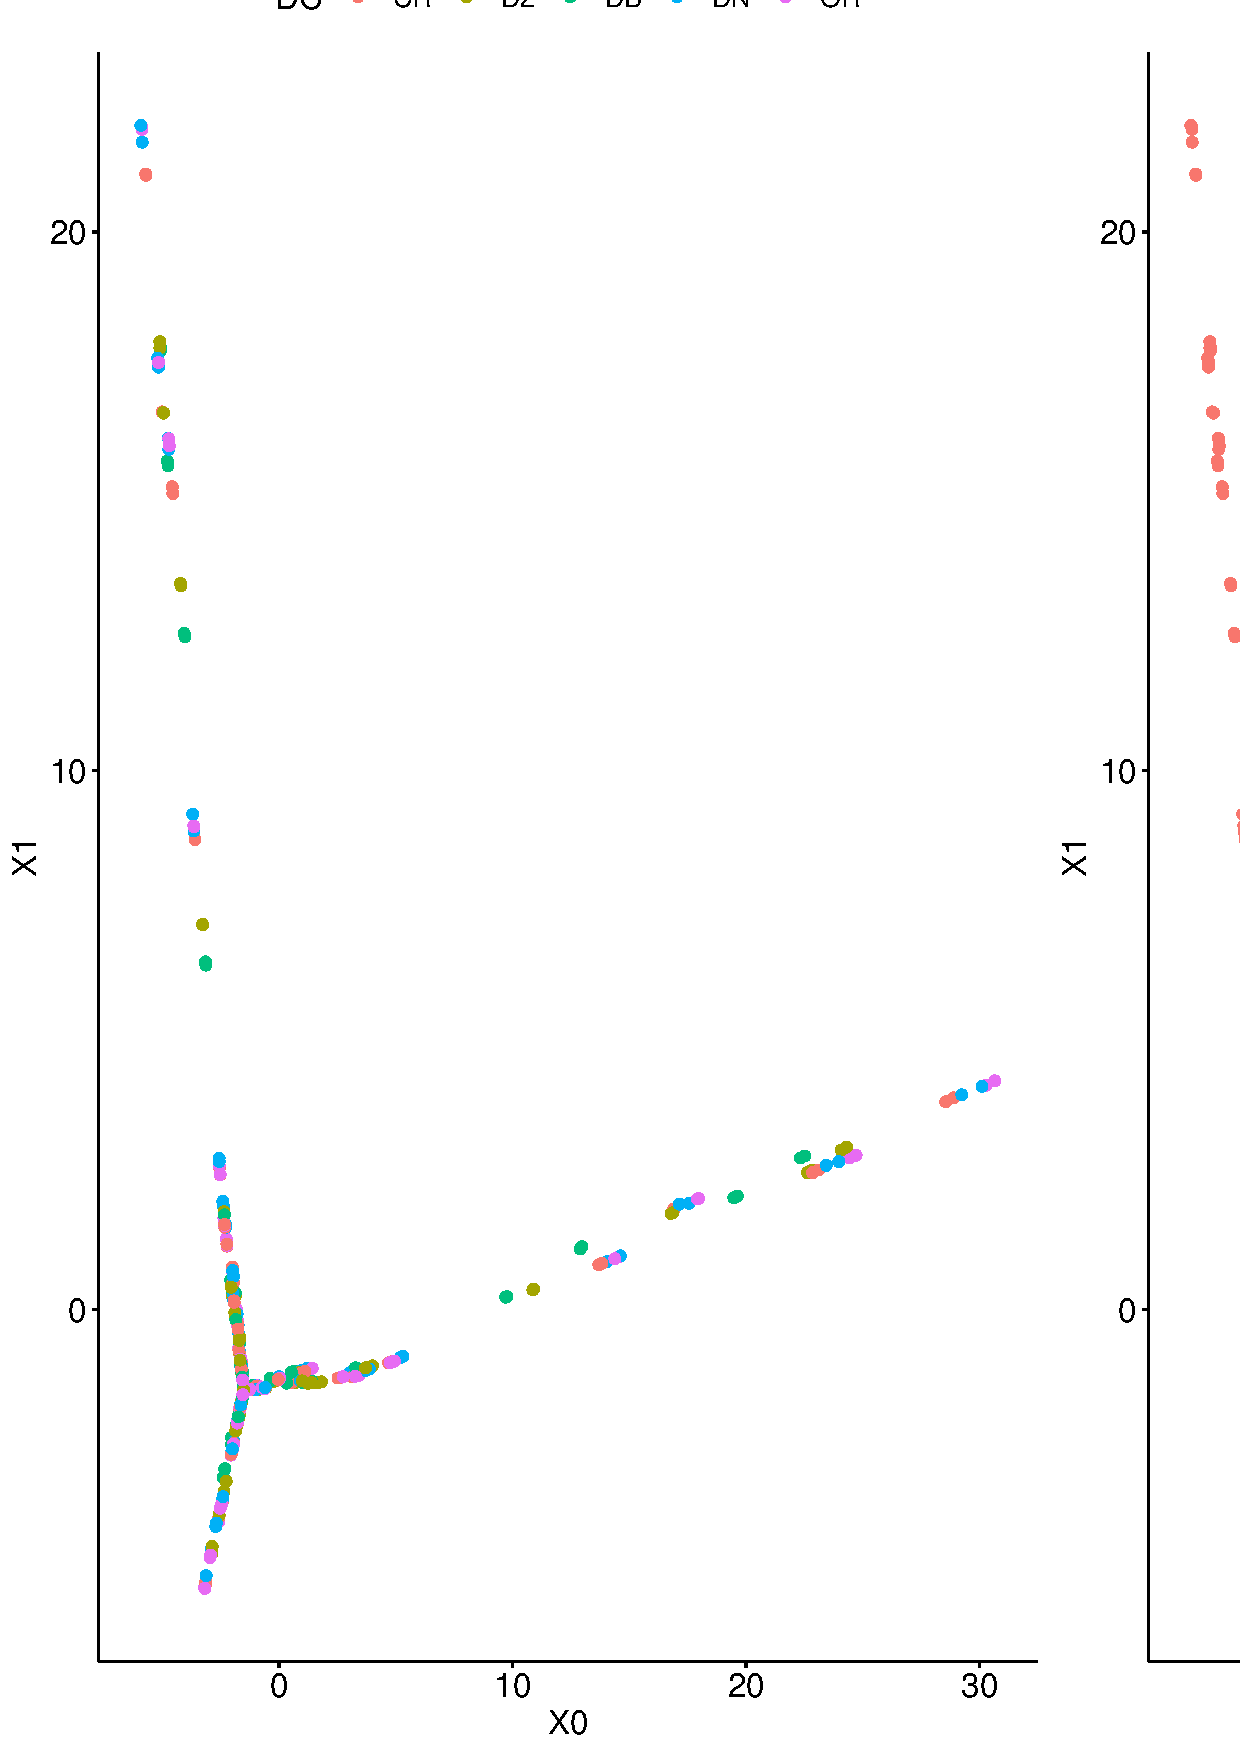
\includegraphics[width=1.0\linewidth]{figure_s1.pdf}
    \DIFaddendFL \end{figure}
    \DIFaddbegin \begin{figure}[H]
      \centering
        \caption{
          \textbf{\DIFaddFL{The networks which were filtered during the }\ac{op} \DIFaddFL{step are less variable}}
          \DIFaddFL{All combinations of inferred networks are shown as points on a PCA plot and shows the variation in the inferred networks in the first two principal axes (similar to Figure~\ref{fig:figure6}B).
          Each point on the PCA plot represents a network inferred using different combinations of tools and parameters that are available in the }\ac{micone} \DIFaddFL{pipeline.
          The points are colored by the tools or parameters used in the }\ac{dc} \DIFaddFL{step (A) and the }\ac{op} \DIFaddFL{step (B).
          The }\ac{dc} \DIFaddFL{step does not seem to have any correlation with the similarity of networks on the PCA plot, but all the networks with filtering at the }\ac{op} \DIFaddFL{step are similar to each other.
          This further confirms that the variability in the networks decreases upon filtering out the taxonomic entities at low abundance.
        }}
      \label{fig:figure_s1}
    \end{figure}
    \FloatBarrier
    \newpage
\DIFaddend 

    \DIFdelbegin %DIFDELCMD < \begin{figure}[h]
%DIFDELCMD <     %%%
\DIFdelendFL %DIF >  TODO: Verify this about t-SNE
    \DIFaddbeginFL \begin{figure}[H]
      \DIFaddendFL \centering
      \DIFdelbeginFL %DIFDELCMD < \includegraphics[width=\linewidth]{figureS2.pdf}
%DIFDELCMD <     %%%
%DIFDELCMD < \caption{%
{%DIFAUXCMD
\textbf{\DIFdelFL{Heatmaps showing the weighted and unweighted unifrac distances for the hard palate dataset analysis}}%DIFAUXCMD
\DIFdelFL{.
      (A) weighted unifrac distances and (B) unweighted unifrac distances between the representative sequences generated by different denoising and clustering algorithms.
      These results are in agreement with the stool microbiome dataset.
    }}
    %DIFAUXCMD
%DIFDELCMD < \label{fig:figureS2}
%DIFDELCMD <   %%%
\DIFdelendFL \DIFaddbeginFL 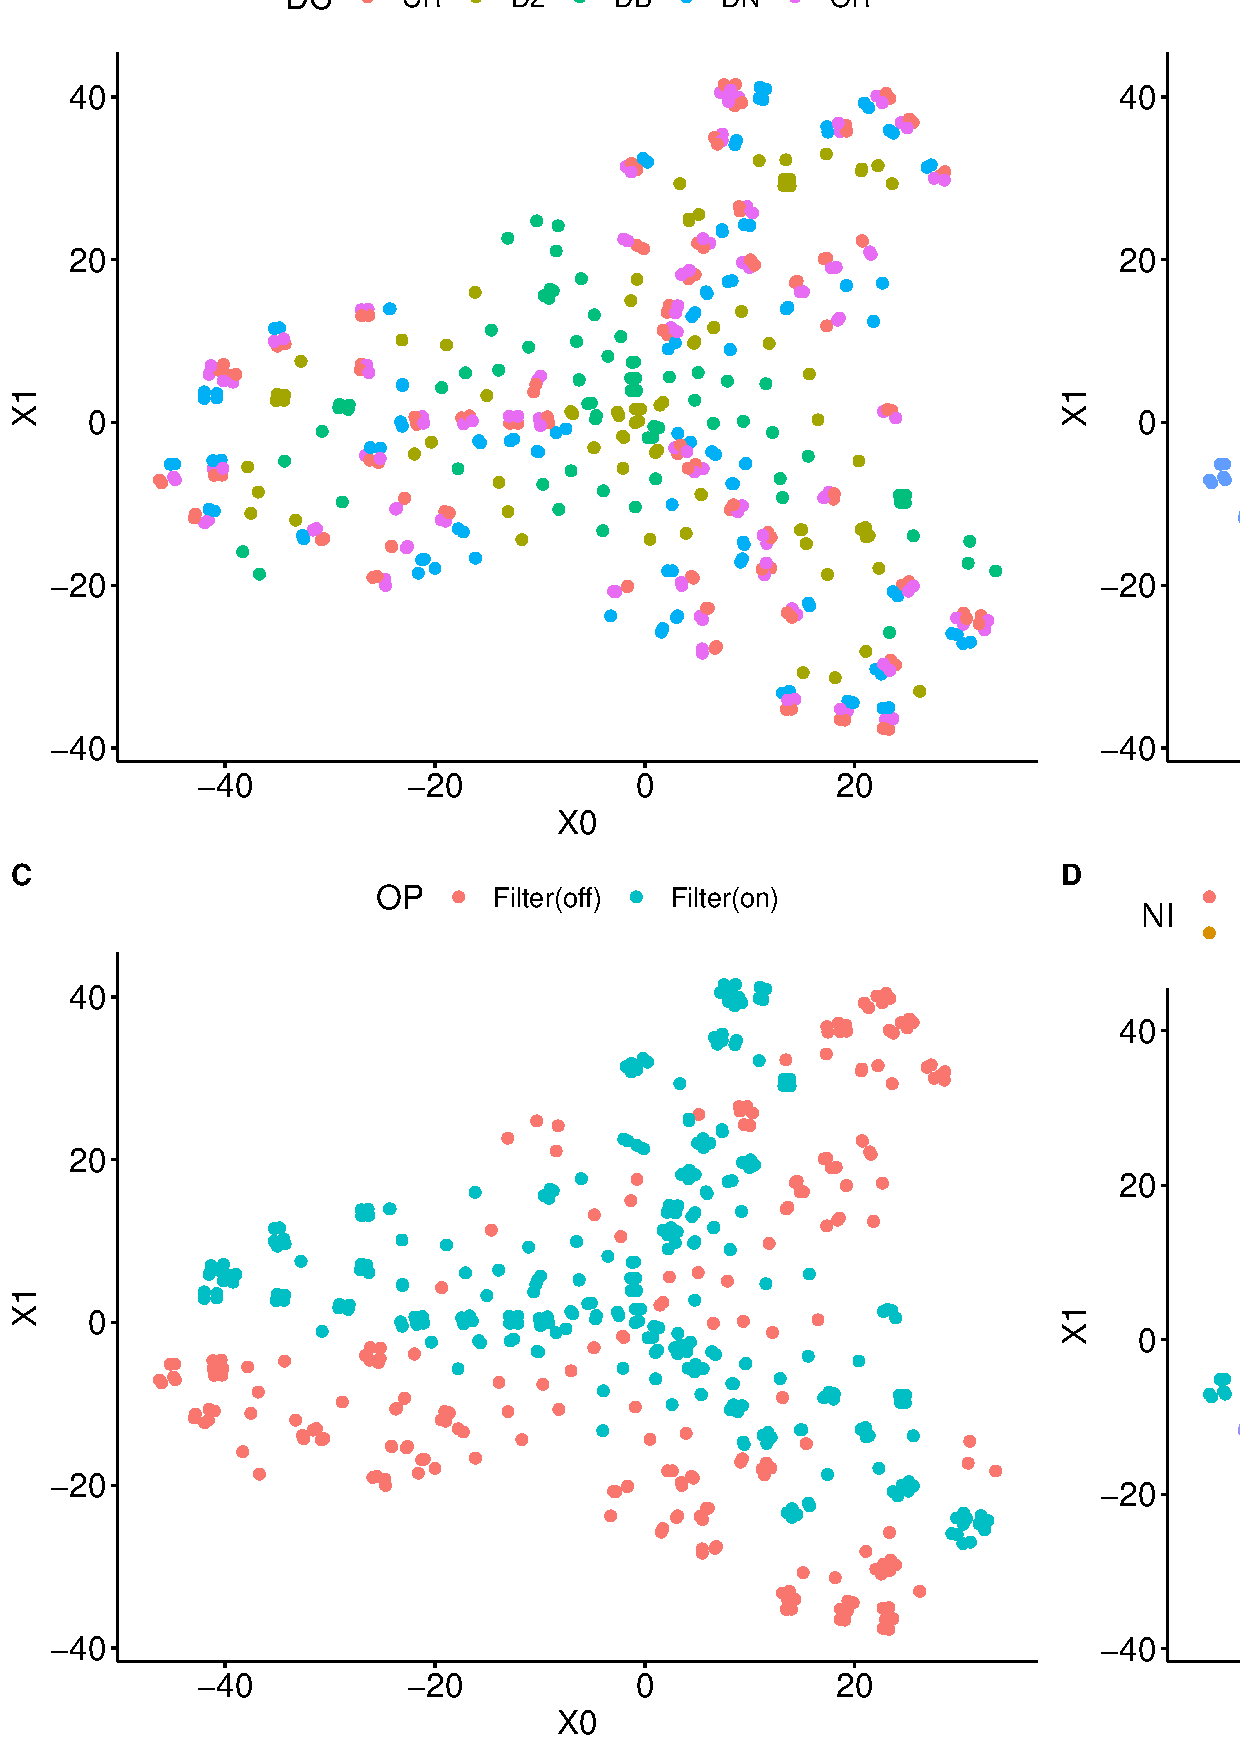
\includegraphics[width=1.0\linewidth]{figure_s2.pdf}
    \DIFaddendFL \end{figure}
    \DIFaddbegin \begin{figure}[H]
      \centering
        \caption{
          \textbf{\DIFaddFL{The t-SNE plot of all the inferred networks clusters the networks based on the taxonomy reference database used}}\DIFaddFL{.
          Each point on the t-SNE plot represents a network inferred using different combinations of tools and parameters that are available in the }\ac{micone} \DIFaddFL{pipeline.
          The points are colored by the tools and parameters used in }\ac{dc} \DIFaddFL{step (A), }\ac{ta} \DIFaddFL{step (B), }\ac{op} \DIFaddFL{step (C) and }\ac{ni} \DIFaddFL{step (D).
          The separation of the points based on taxonomy reference database shows that the points might cluster based on reference database in high-dimensional space.
        }}
      \label{fig:figure_s2}
    \end{figure}
    \FloatBarrier
    \newpage
\DIFaddend 

    \DIFdelbegin %DIFDELCMD < \begin{figure}[h]
%DIFDELCMD <     %%%
\DIFdelendFL \DIFaddbeginFL \begin{figure}[H]
      \DIFaddendFL \centering
      \DIFdelbeginFL %DIFDELCMD < \includegraphics[width=\linewidth]{figureS3.pdf}
%DIFDELCMD <     %%%
%DIFDELCMD < \caption{%
{%DIFAUXCMD
\textbf{\DIFdelFL{The distributions of the average weighted UniFrac distance between the expected sequence profile and the calculated sequence profile in the synthetic datasets}}%DIFAUXCMD
\DIFdelFL{.
      We observe no significant difference between the various methods on the synthetic datasets used for this study.
    }}
    %DIFAUXCMD
%DIFDELCMD < \label{fig:figureS3}
%DIFDELCMD <   %%%
\DIFdelendFL \DIFaddbeginFL 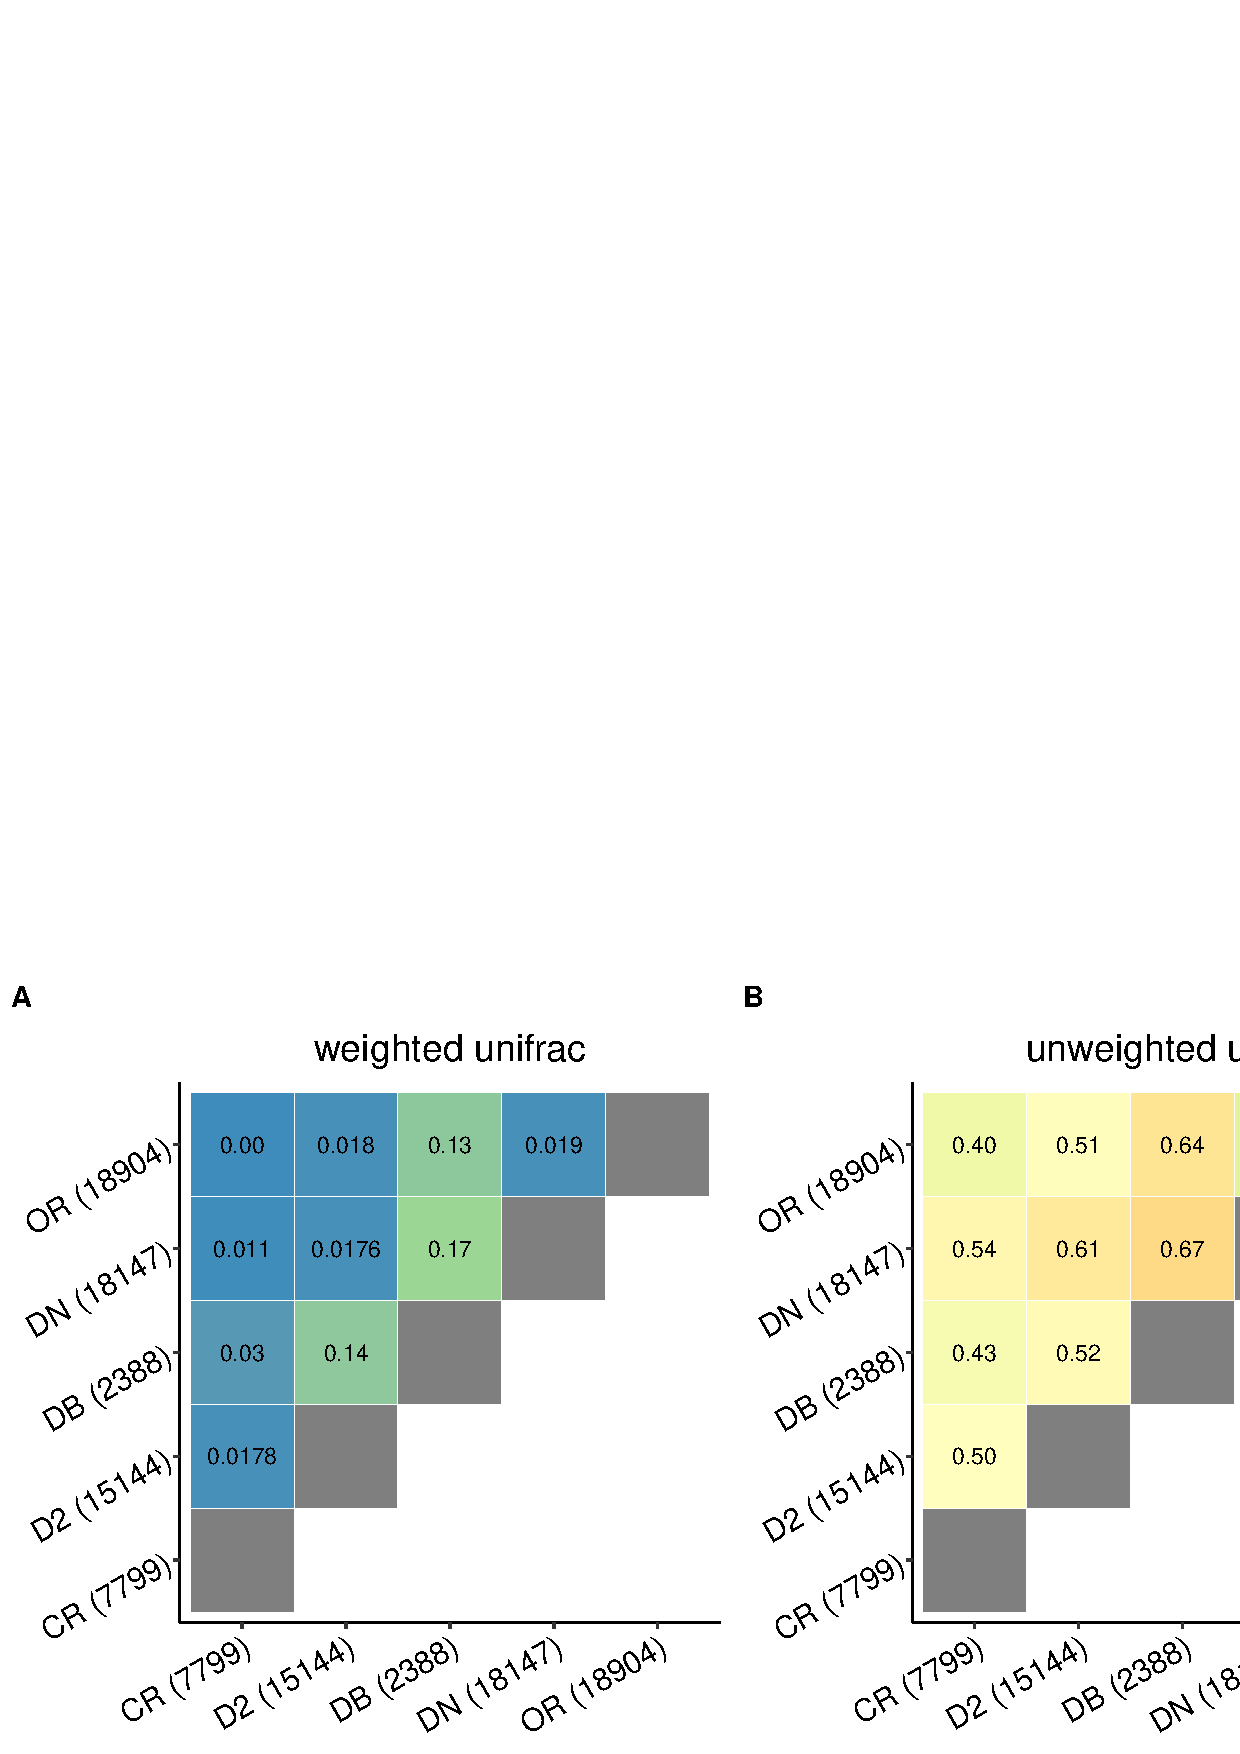
\includegraphics[width=1.0\linewidth]{figure_s3.pdf}
    \DIFaddendFL \end{figure}
    \DIFaddbegin \begin{figure}[H]
      \centering
        \caption{
          \textbf{\DIFaddFL{The UniFrac distance between the 1000 most abundant representative sequences is higher than that when all sequences are considered}}\DIFaddFL{.
          Each value is the average UniFrac distance between the reference sequences generated by the various methods in the }\ac{dc} \DIFaddFL{step (similar to Figure~\ref{fig:figure2}).
          There is an increase in both weighted and unweighted UniFrac distances compared to when all the representative sequences are considered.
          This shows that the 1000 most abundant representative sequences generated by the methods are not as similar to each other.
          And since the weighted UniFrac is much smaller than the unweighted UniFrac distance, we can conclude that those reference sequences that are present in the middle of the abundance distribution are dissimilar.
        }}
      \label{fig:figure_s3}
    \end{figure}
    \FloatBarrier
    \newpage
\DIFaddend 

    %DIF <    \begin{figure}[h]
%DIF <      \centering
%DIF <      \includegraphics[width=0.9\linewidth]{pdf/all_denoise_reg.pdf}
%DIF <      \caption*{All pairwise correlations comparing the similarity between different denoising and clustering methods}
%DIF <      \label{fig:figureS4}
%DIF <    \end{figure}
\DIFdelbegin %DIFDELCMD < 

%DIFDELCMD <   \begin{figure}[h]
%DIFDELCMD <     %%%
\DIFdelendFL \DIFaddbeginFL \begin{figure}[H]
      \DIFaddendFL \centering
      \DIFdelbeginFL %DIFDELCMD < \includegraphics[width=\linewidth]{figureS4.pdf}
%DIFDELCMD <     %%%
%DIFDELCMD < \caption{%
{%DIFAUXCMD
\textbf{\DIFdelFL{(A)}} %DIFAUXCMD
\DIFdelFL{Taxonomy composition of the 20 most abundant genera predicted for the stool microbiome dataset generated using different taxonomy references databases: Greengenes, SILVA and NCBI.
      The legend shows the common and the unique genera among the taxonomy assignments.
  }}
    %DIFAUXCMD
%DIFDELCMD < \label{fig:figureS4}
%DIFDELCMD <   %%%
\DIFdelendFL \DIFaddbeginFL 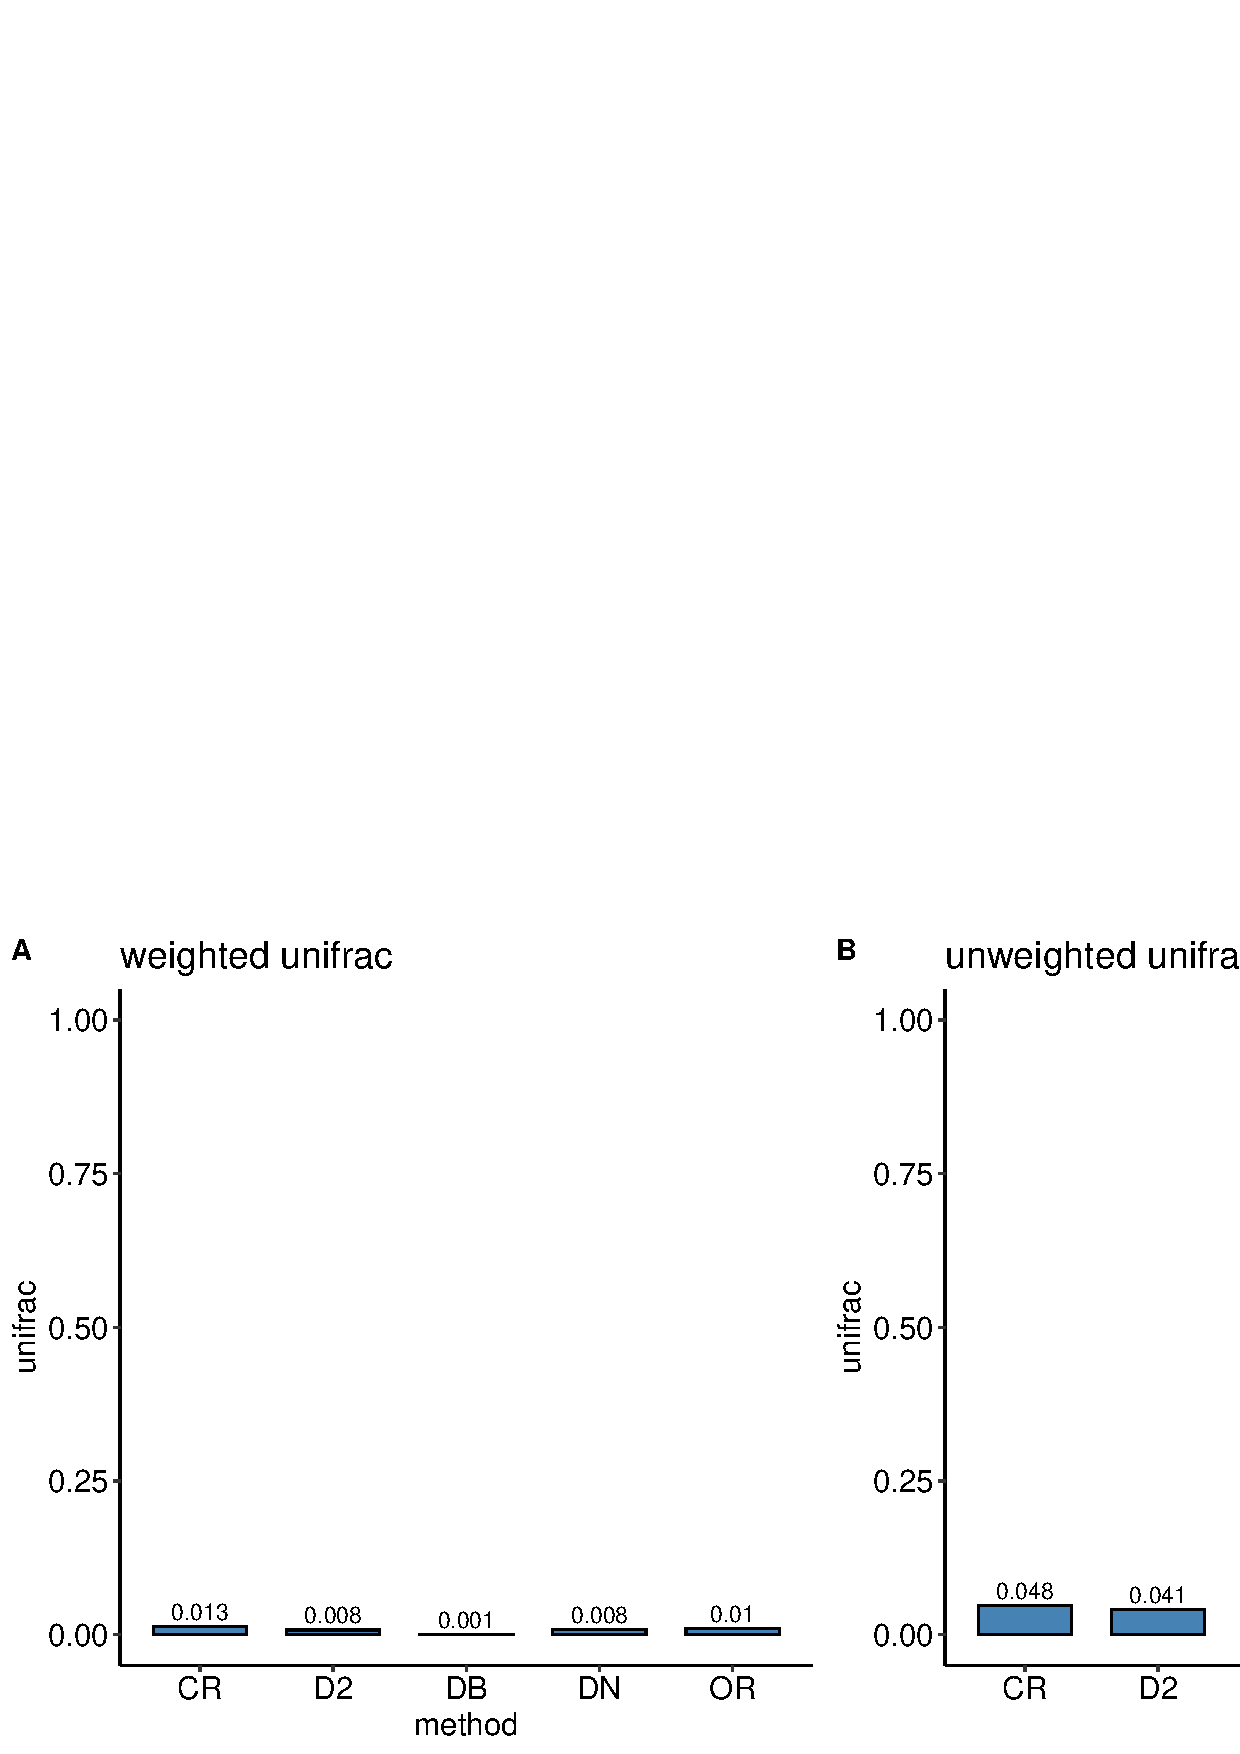
\includegraphics[width=1.0\linewidth]{figure_s4.pdf}
    \DIFaddendFL \end{figure}
    \DIFaddbegin \begin{figure}[H]
      \centering
        \caption{
          \textbf{\DIFaddFL{The weighted and unweighted UniFrac distances between representative sequences generated using remove bimera and uchime for each denoising method are low.}}
          \DIFaddFL{The two chimera checking methods, uchime and remove bimera, produce similar outputs.
          With the exception of de novo and open reference under the unweighted UniFrac metric, all the other methods have low dissimilarity.
          This is especially true for the }\ac{dada2} \DIFaddFL{and Deblur methods which are the recommended denoising methods in the }\ac{micone} \DIFaddFL{pipeline.
          Therefore, remove bimera is recommended as the default chimera method if one is using }\ac{dada2} \DIFaddFL{and uchime-denovo when one is using Deblur, since these methods were developed for these respective algorithms (}\ac{qiime2} \DIFaddFL{uses uchime-denovo in the Deblur workflow).
        }}
      \label{fig:figure_s4}
    \end{figure}
    \FloatBarrier
    \newpage
\DIFaddend 

    \DIFdelbegin %DIFDELCMD < \begin{figure}[h]
%DIFDELCMD <     %%%
\DIFdelendFL \DIFaddbeginFL \begin{figure}[H]
      \DIFaddendFL \centering
      \DIFdelbeginFL %DIFDELCMD < \includegraphics[width=\linewidth]{figureS5.pdf}
%DIFDELCMD <     %%%
%DIFDELCMD < \caption{%
{%DIFAUXCMD
\DIFdelFL{The bray-curtis dissmilarity between the expected taxonomic composition and generated taxonomic composiion for the synthetic datasets.
  }}
  %DIFAUXCMD
%DIFDELCMD < \label{fig:figureS5}
%DIFDELCMD <   %%%
\DIFdelendFL \DIFaddbeginFL 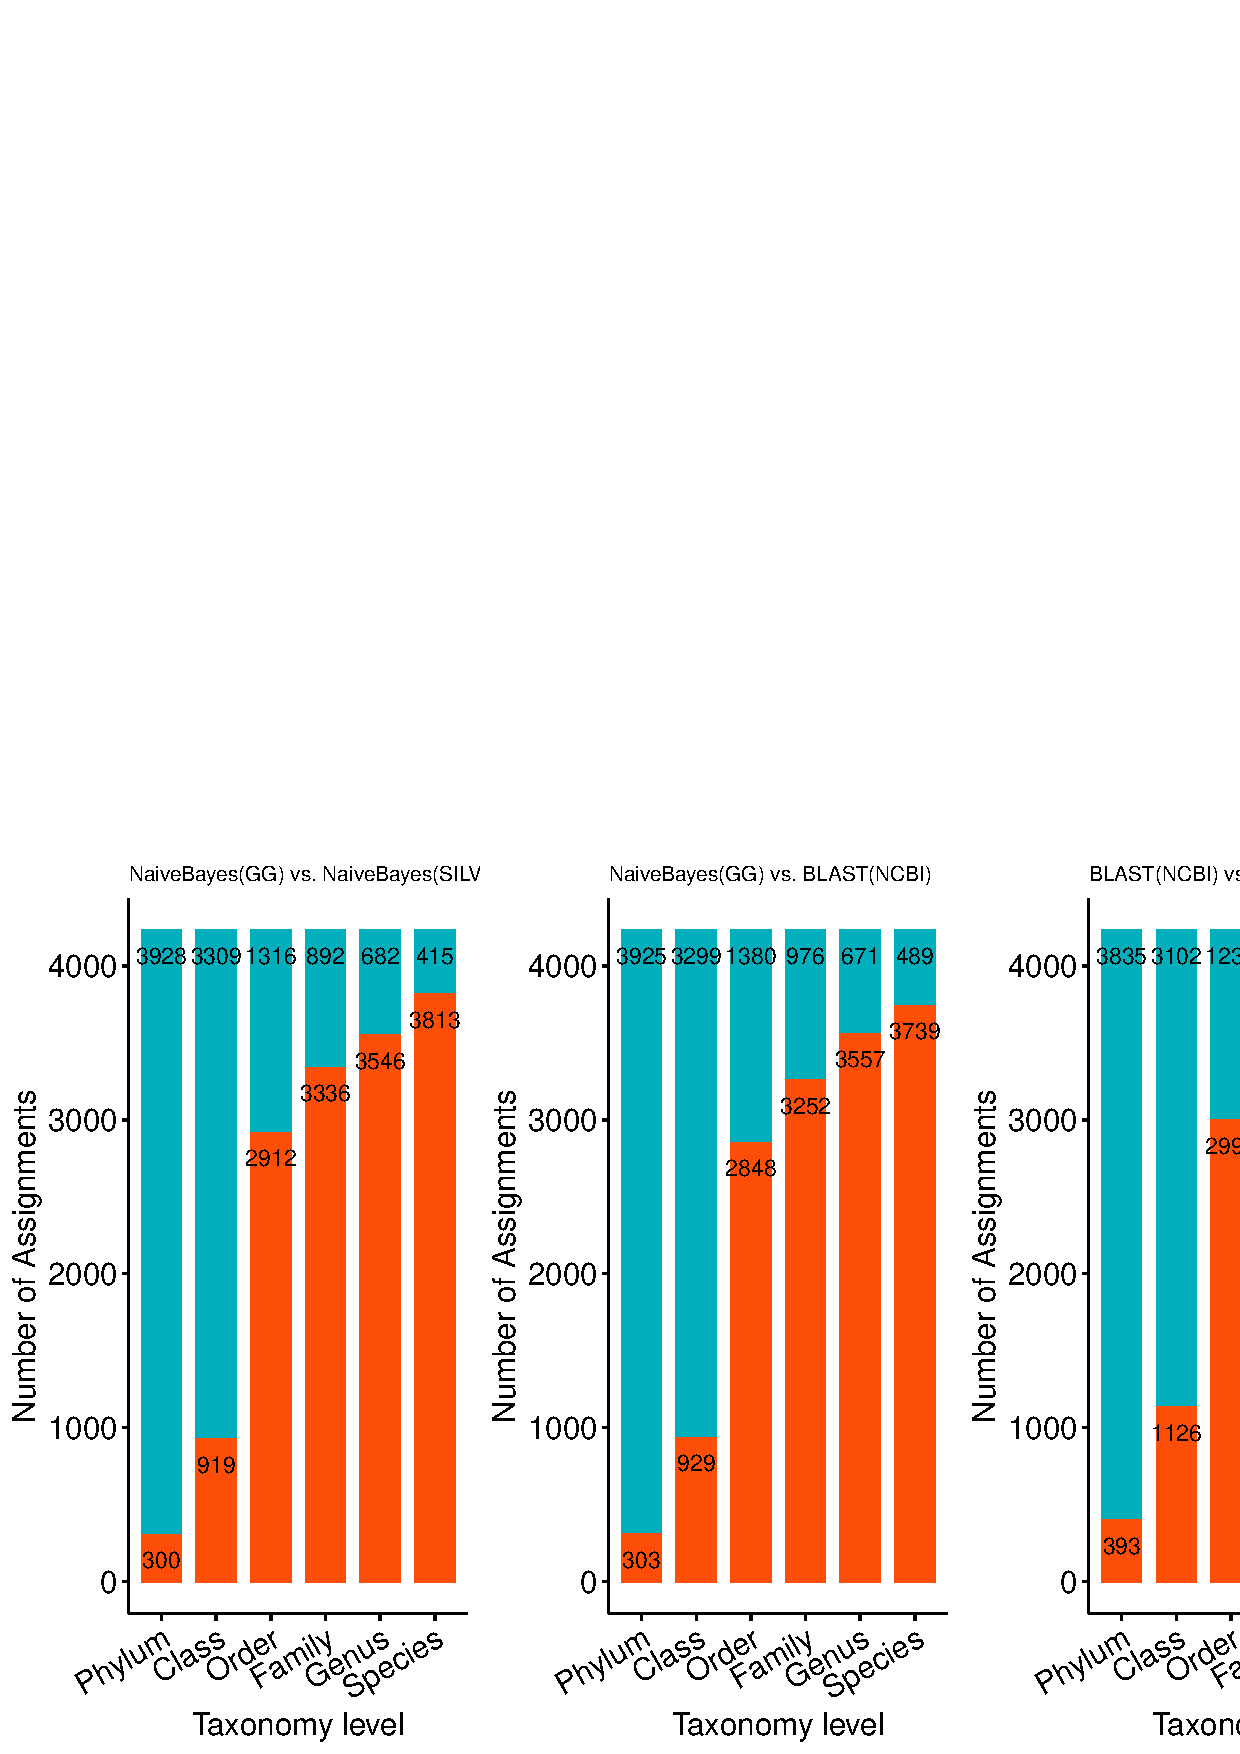
\includegraphics[width=1.0\linewidth]{figure_s5.pdf}
    \DIFaddendFL \end{figure}
    \DIFaddbegin \begin{figure}[H]
      \centering
        \caption{
          \textbf{\DIFaddFL{The pairwise comparison of assignments generated using different databases for all representative sequences has a higher proportion of mismatches}}\DIFaddFL{.
          The comparison made here is similar to Figure~\ref{fig:figure3}B, but instead of the top 100 taxonomic entities (by abundance), all the assignments from one database are matched with those from the other two databases.
          Higher percentage of mismatches implies that the matching of the taxonomies in the more abundant sequences (top 100) are more consistent.
        }}
      \label{fig:figure_s5}
    \end{figure}
    \FloatBarrier
    \newpage
\DIFaddend 

  %DIF <    \begin{figure}[h]
%DIF <      \centering
%DIF <      \includegraphics[width=\linewidth]{figureS6.pdf}
%DIF <      \caption{
%DIF <        Calculation of presence threshold that is applied on the OTU table in the OTU processing (OP) step of the pipeline.
%DIF <        This presence threhold $p_t$ is dependent on the number of samples in the dataset and the required correlation stength threshold.
%DIF <    }
%DIF <      \label{fig:figureS6}
%DIF <    \end{figure}
\DIFdelbegin %DIFDELCMD < 

%DIFDELCMD <   \begin{figure}[h]
%DIFDELCMD <     %%%
\DIFdelendFL \DIFaddbeginFL \begin{figure}[H]
    \DIFaddendFL \centering
    \DIFdelbeginFL %DIFDELCMD < \includegraphics[width=\linewidth]{figureS8.pdf}
%DIFDELCMD <     %%%
%DIFDELCMD < \caption{%
{%DIFAUXCMD
\DIFdelFL{The similarity between the networks generated using the different network inference algorithms for stool dataset (A) and the hard palate dataset (B).
      The similarity between the various methods was found to vary with the dataset used.
  }}
    %DIFAUXCMD
%DIFDELCMD < \label{fig:figureS8}
%DIFDELCMD <   %%%
\DIFdelendFL \DIFaddbeginFL 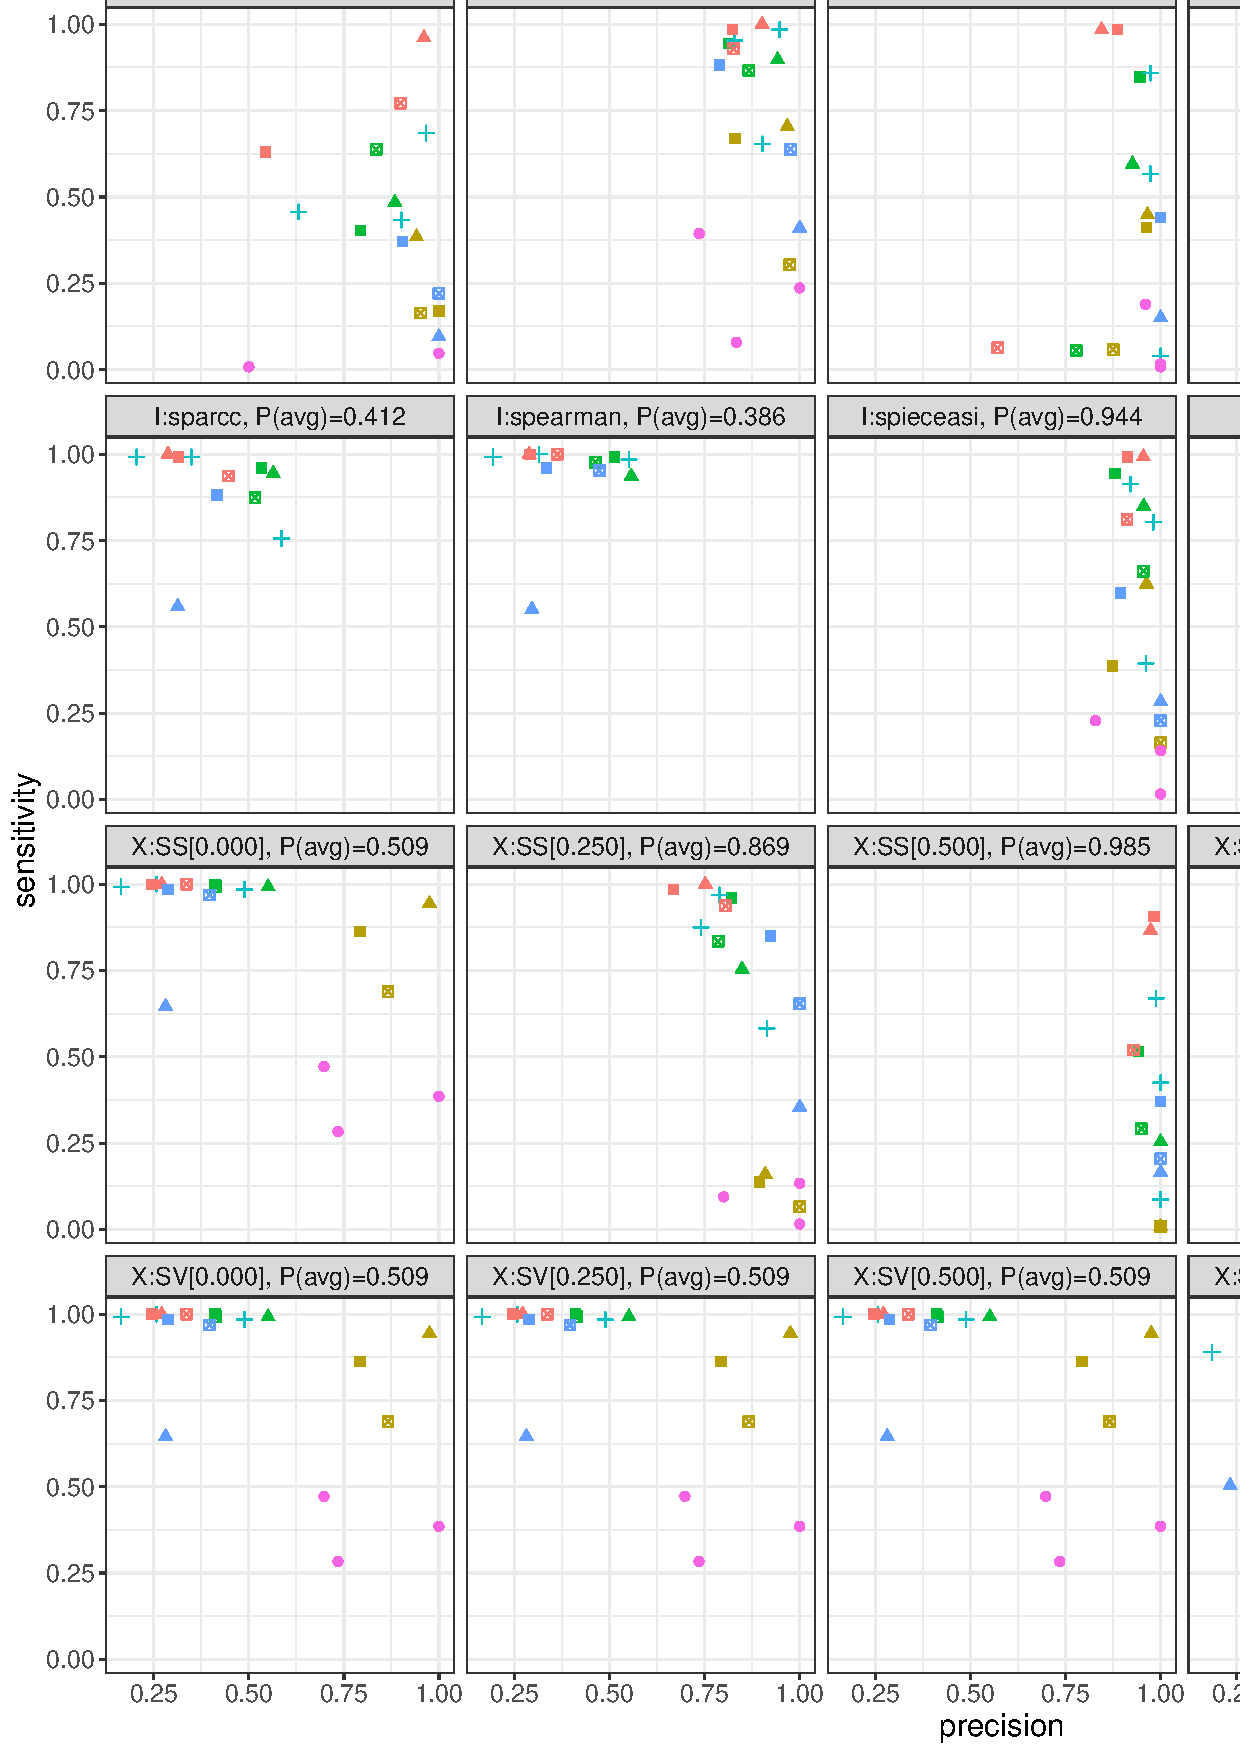
\includegraphics[width=1.0\linewidth]{figure_s6.pdf}
  \DIFaddendFL \end{figure}
  \DIFaddbegin \begin{figure}[H]
    \centering
      \caption{
        \textbf{\DIFaddFL{The precision and sensitivity of the inferred networks on the NorTA synthetic interaction data when Pearson and Spearman are included in the consensus calculation}}\DIFaddFL{.
        The ``I'' prefix indicates the individual network inference methods and the ``X'' prefix denotes the different consensus based methods.
        The different consensus based methods used are: pvalue merging (PM), scaled-sum (SS) and simple voting (SV) method.
        With the addition of Pearson and Spearman in the consensus calculation we observe a decrease in the average precision scores of both the consensus algorithms (compared to Figure~\ref{fig:figure5}.
        The overall best precision was still consistently obtained by the scaled-sum method (0.985, 0.963 and 1.000), but the performance was not stable to an increase in the parameter value.
        The simple voting method when using presence of edges in all inferred networks as a requirement (parameter value 1.000), again outperforms }\ac{spieceasi} \DIFaddFL{on average precision (0.961).
      }}
    \label{fig:figure_s6}
  \end{figure}
  \FloatBarrier
  \newpage
\DIFaddend 

  \DIFdelbegin %DIFDELCMD < \begin{figure}[h]
%DIFDELCMD <     %%%
\DIFdelendFL \DIFaddbeginFL \begin{figure}[H]
    \DIFaddendFL \centering
    \DIFdelbeginFL %DIFDELCMD < \includegraphics[width=0.8\linewidth]{pdf/denoise_network.pdf}
%DIFDELCMD <     %%%
%DIFDELCMD < \caption{%
{%DIFAUXCMD
\DIFdelFL{A network showing union (A) and intersection (B) of networks generated using different denoising and clustering tools on the Stool dataset.}}
    %DIFAUXCMD
%DIFDELCMD < \label{fig:figureS5}
%DIFDELCMD <   %%%
\DIFdelendFL \DIFaddbeginFL 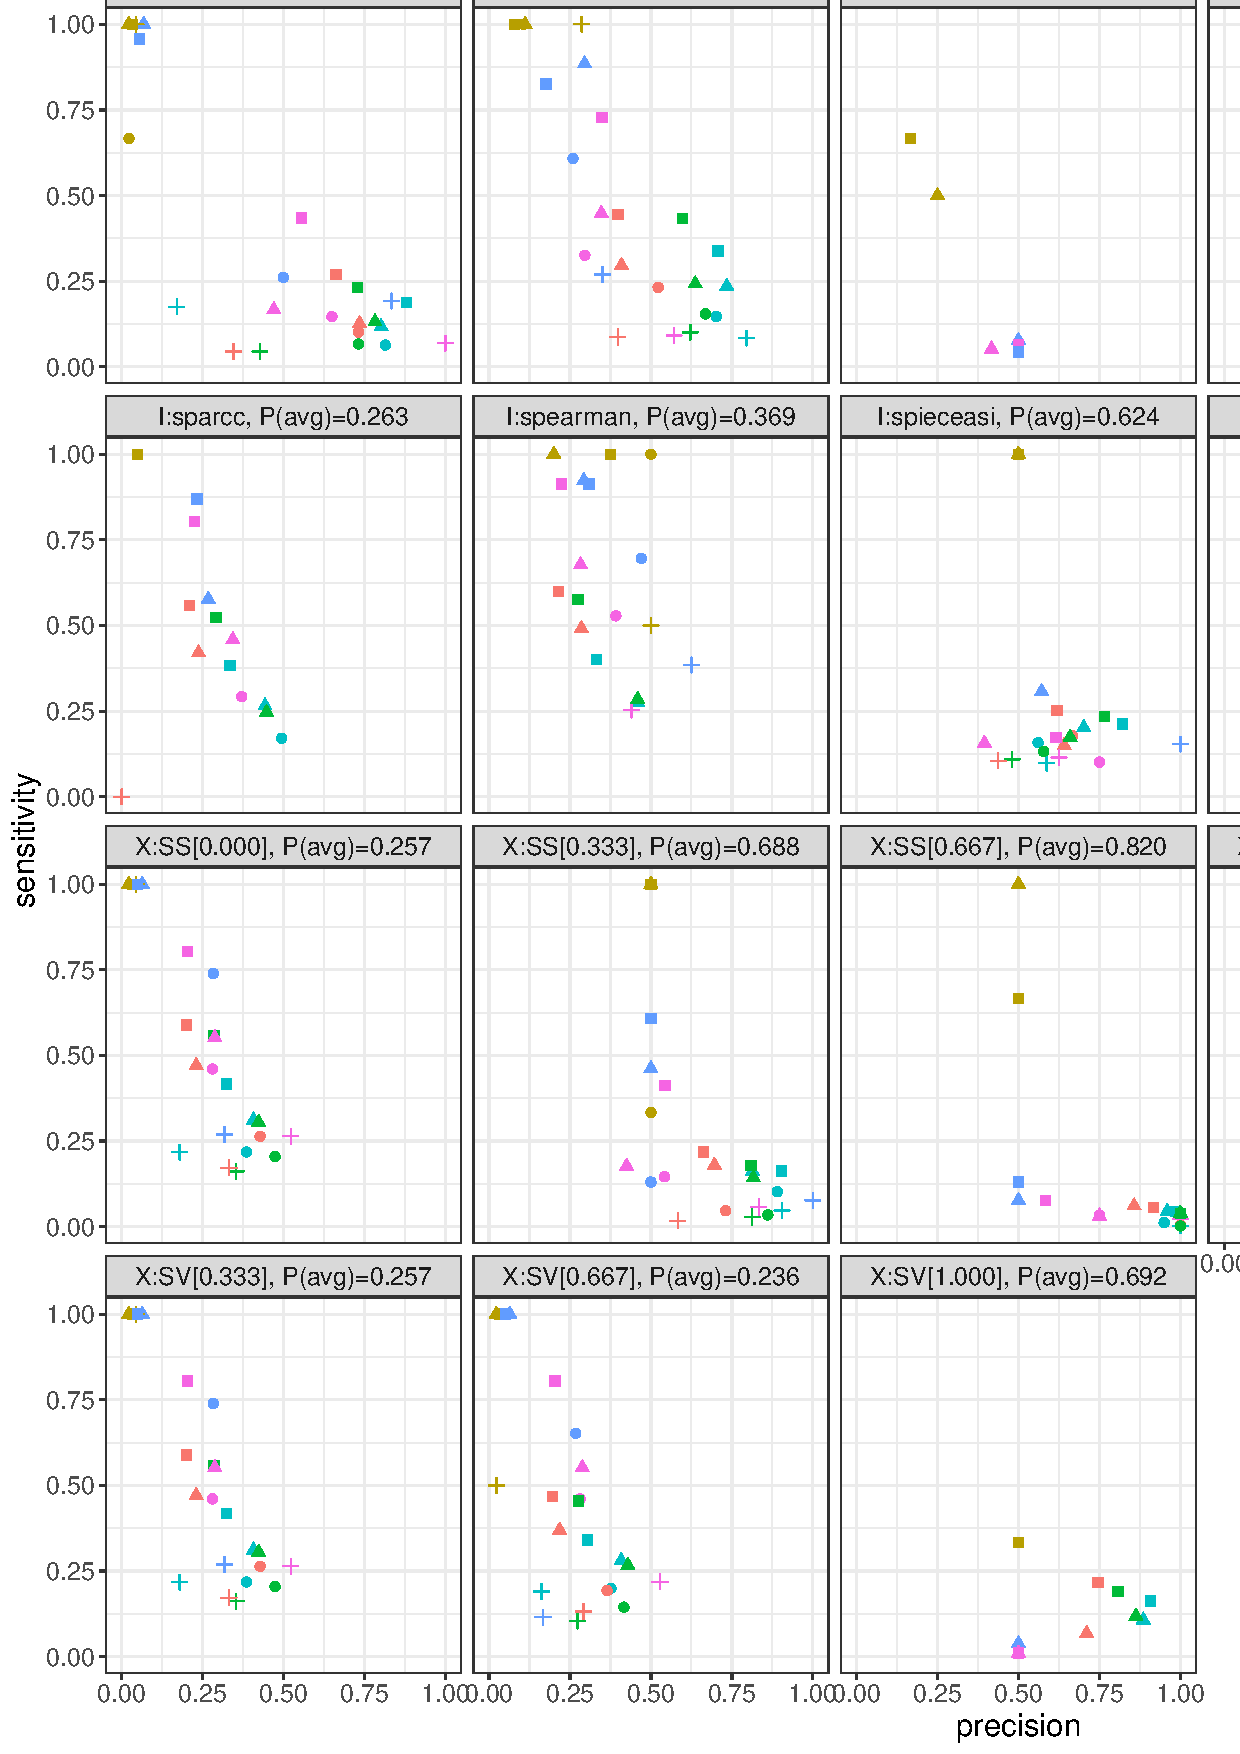
\includegraphics[width=1.0\linewidth]{figure_s7.pdf}
  \DIFaddendFL \end{figure}
  \DIFaddbegin \begin{figure}[H]
    \centering
      \caption{
        \textbf{\DIFaddFL{The precision and sensitivity of the inferred networks on the seqtime synthetic interaction data.}}
        \DIFaddFL{The ``I'' prefix indicates the individual network inference methods and the ``X'' prefix denotes the different consensus based methods.
        The different consensus based methods used are: pvalue merging (PM), scaled-sum (SS) and simple voting (SV) method.
        Pearson and Spearman methods are not used in the calculation of the consensus.
        Among all the independent network inference methods, }\ac{spieceasi} \DIFaddFL{has the best average precision (0.624), but the overall best precision was consistently obtained by the scaled-sum method (0.688, 0.820 and 1.000).
        The simple voting method when using presence of edges in all inferred networks as a requirement (parameter value 1.000), also outperforms }\ac{spieceasi} \DIFaddFL{on average precision (0.692).
        These results show that the scaled-sum method is not only much better suited for inferring robust and accurate interactions from count data regardless of the distributions and topologies.
        But, it is also capable of accurately extracting real interactions (gLV interactions) from count data.
      }}
    \label{fig:figure_s7}
  \end{figure}
  \FloatBarrier
  \newpage

  \subsection*{\DIFadd{Processing the FMT data}}

    \subsubsection*{\DIFadd{Data download and pre-processing}}
    \DIFadd{The main biological dataset used in this study was the collection of 16S rRNA sequencing reads from stool samples (healthy and autistic individuals) for a fecal microbiome transplant study~\mbox{%DIFAUXCMD
\cite{Kang2017}}\hskip0pt%DIFAUXCMD
.
    The data containing the 16S sequencing reads (V4 region) was downloaded from Qiita~\mbox{%DIFAUXCMD
\cite{qiita} }\hskip0pt%DIFAUXCMD
(study ID: 10532).
    Only runs 2, 3, and 4 were used for the subsequent analysis as these runs consisted of paired-end sequencing data and run 1 contained single-end data.
    The sample metadata was updated to contain only BMI, sex, height, weight and experimental group.
    This was necessary as two of the network inference algorithms (}\ac{mldm} \DIFadd{and FlashWeave) required information about environmental heterogeneity.
    However, these environmental correlations were not included in the current analyses.
}

    \subsubsection*{\DIFadd{Processing using the }\ac{micone} \DIFadd{pipeline}}
    \DIFadd{The data was then processed using the }\ac{micone} \DIFadd{pipeline starting at the }\ac{sp} \DIFadd{step and ending at the }\ac{ni} \DIFadd{step with the consensus algorithm.
    The configuration files (main.nf and nextflow.config) used to run the }\ac{micone} \DIFadd{pipeline as well the details of the pipeline execution (dag, report, timeline and trace) are in the "runs/FMT" directory of the data and scripts repository (}\href{https://github.com/segrelab/MiCoNE-pipeline-paper}{\DIFadd{https://github.com/segrelab/MiCoNE-pipeline-paper}}\DIFadd{)
    %DIF >  TODO: Store pipeline results
    The results of the pipeline execution for reproducing the analyses in the manuscript are stored on Zenodo}[\DIFadd{REF}] \DIFadd{at ...
}

  \subsection*{\DIFadd{Processing the mock data}}

    \subsubsection*{\DIFadd{Data download and pre-processing}}
    \DIFadd{The mock datasets, mock4, mock12 and mock16 used for this study, were obtained from mockrobiota~\mbox{%DIFAUXCMD
\cite{Bokulich2016}}\hskip0pt%DIFAUXCMD
.
    Mock 4 is a mock community composed of 21 bacterial strains represented in equal abundances in two replicate samples, and the same strains represented in uneven abundances in two other replicate samples.
    Mock 12 is composed of 27 bacterial strains containing closely related taxa, the members of which were chosen in part for their well-separated 16S rRNA gene sequences. Some pairs of strains differ by as little as one nucleotide, but all the strains are distinguishable over the sequenced region of the 16S rRNA gene.
    Mock 16 is a mock community composed of even amounts of purified genomic DNA from 49 bacteria and 10 archaea.
    The datasets did not require any preprocessing and could be directly used as input to the pipeline
}

    \subsubsection*{\DIFadd{Processing using the }\ac{micone} \DIFadd{pipeline}}
    \DIFadd{The data was processed using the }\ac{micone} \DIFadd{pipeline starting at the }\ac{sp} \DIFadd{step and ending at the }\ac{op} \DIFadd{step with the filtered taxonomic tables as the final output.
    The configuration files (main.nf and nextflow.config) used to run the }\ac{micone} \DIFadd{pipeline as well the details of the pipeline execution (dag, report, timeline and trace) are in the "runs/mock*" directory of the data and scripts repository (}\href{https://github.com/segrelab/MiCoNE-pipeline-paper}{\DIFadd{https://github.com/segrelab/MiCoNE-pipeline-paper}}\DIFadd{)
    %DIF >  TODO: Store pipeline results
    The results of the pipeline execution for reproducing the analyses in the manuscript are stored on Zenodo at ...
}

  \subsection*{\DIFadd{Synthetic interaction data}}

    \subsubsection*{\DIFadd{Data generation}}
    \DIFadd{The synthetic interaction data for the study were generated using two methods.
    The first method, ``seqtime''~\mbox{%DIFAUXCMD
\cite{faustSignaturesEcologicalProcesses2018} }\hskip0pt%DIFAUXCMD
utilized generalized Lotka-Volterra (gLV) equations to model the microbial community dynamics and made use of the Klemm–Eguı́luz algorithm to generate clique-based interaction networks~\mbox{%DIFAUXCMD
\cite{Rottjers2018}}\hskip0pt%DIFAUXCMD
.
    We used the seqtime R package to simulate communities with different numbers of species and samples (see Methods for details).
    The second method, ``NorTA'' used the Normal to Anything (NorTA) approach coupled with a given interaction network topology to generate the abundance distribution of the microbial community~\mbox{%DIFAUXCMD
\cite{Kurtz2015}}\hskip0pt%DIFAUXCMD
.
    We used the spieceasi R package to simulate communities with different abundance distributions and network topologies (see Methods for details).
    The scripts to generate these datasets can be found in the synthetic data and scripts repository (}\href{https://github.com/segrelab/MiCoNE-synthetic-data}{\DIFadd{https://github.com/segrelab/MiCoNE-synthetic-data}}\DIFadd{)
}

    \subsubsection*{\DIFadd{Processing using the }\ac{micone} \DIFadd{pipeline}}
    \DIFadd{The data was processed using the }\ac{micone} \DIFadd{pipeline using only the }\ac{ni} \DIFadd{step with the consensus networks as the final output.
    The configuration files (main.nf and nextflow.config) used to run the }\ac{micone} \DIFadd{pipeline as well the details of the pipeline execution (dag, report, timeline and trace) are in the "runs/norta" and "runs/seqtime" directories of the data and scripts repository (}\href{https://github.com/segrelab/MiCoNE-pipeline-paper}{\DIFadd{https://github.com/segrelab/MiCoNE-pipeline-paper}}\DIFadd{)
    %DIF >  TODO: Store pipeline results
    The results of the pipeline execution for reproducing the analyses in the manuscript are stored on Zenodo at ...
}


  \subsection*{\DIFadd{Network metrics}}

  \DIFadd{In Table~\ref{tab:network_metrics} we show various global network metrics calculated for each tool in the pipeline.
  All the networks that make use of a particular tool are grouped together, and the following average metrics are calculated for each group:
  }\begin{enumerate}
    \item \DIFadd{The average shortest path length describes the average of all the shortest paths in the graph. No number is reported if the graph is not connected, therefore, the results indicate that none of the networks that make use of }\ac{harmonies}\DIFadd{, }\ac{cozine}\DIFadd{, }\ac{spring}\DIFadd{, }\ac{spieceasi} \DIFadd{and Pearson are connected.
    }\item \DIFadd{The average clustering is the average clustering coefficient of the graph. The closer the value is to 1.0, the more densely connected is the graph. We can observe that the networks that use correlation-based methods have the highest values while the direct-association based methods have the lowest.
    }\item \DIFadd{The number of connected components is the highest for the direct-association based methods and the lowest for the correlation-based methods. In the case of propr, all the networks have only one giant component.
    }\item \DIFadd{The modularity metric is the modularity over all partitions in a graph calculated using a label propagation algorithm~\mbox{%DIFAUXCMD
\cite{cordascoCommunityDetectionSemisynchronous2010}}\hskip0pt%DIFAUXCMD
. Positive values imply that there are more edges between vertices of the same type than we would expect by chance, and negative implies that there are less. The networks inferred by }\ac{mldm} \DIFadd{report very few edges, and skew the average modularity scores. This could also be an artifact of incomplete converge of the }\ac{mldm} \DIFadd{algorithm for some combinations.
    }\item \DIFadd{Node connectivity refers to the minimum number of nodes that must be removed from the graph to make it disconnected. We observe that only the networks generated using propr have a high value since most of these networks are connected.
    }\item \DIFadd{Degree assortativity coefficient measures the similarity of connections in the graph with respect to the node degree. Again we observe that the direct-association based methods have negative degree assortativity, meaning that there are many hubs in these networks. The correlation-based methods have positive values implying that in these networks nodes with similar degrees attach to one another.
  }\end{enumerate}
  \DIFadd{All the metrics were calculated using the }\texttt{\DIFadd{networkx}} \DIFadd{Python package~\mbox{%DIFAUXCMD
\cite{hagbergExploringNetworkStructure2008}}\hskip0pt%DIFAUXCMD
.
}

  \subsection*{\DIFadd{p-value merging}}

  \DIFadd{Fisher~\mbox{%DIFAUXCMD
\cite{fisher_224a_1948} }\hskip0pt%DIFAUXCMD
proposed that for $k$ independent p-values, each generated by $k$ different methods and denoted by $\bar{P}^i$ (notations are same as used in the "Consensus network and p-value merging" subsection of the Methods), the following will hold true for the statistic $\Psi$:
  }\begin{equation*}
    \DIFadd{\begin{aligned}
      \Psi &= \sum_{i=1}^k -2 \log \left( \bar{P}^i \right) \\
        \Psi &\sim \chi^2_{2k}
    \end{aligned}
  }\end{equation*}

  \DIFadd{Brown~\mbox{%DIFAUXCMD
\cite{brown_400_1975} }\hskip0pt%DIFAUXCMD
extended Fisher's method to dependent p-values by using a re-scaled $\chi^2$ distribution:
  }\begin{equation*}
    \DIFadd{\Psi \sim c \chi^2_{2f}
  }\end{equation*}
  \DIFadd{where, $f$ is the degrees of freedom and $c$ is the scale factor and are given by:
  }\begin{equation*}
    \DIFadd{f = \frac{\mathrm{E}[\Psi]^2}{\mathrm{Var}[\Psi]} ~~~\text{and}~~~ c = \frac{\mathrm{Var}[\Psi]}{2\mathrm{E}[\Psi]} = \frac{k}{f}
  }\end{equation*}

  \DIFadd{Furthermore, Brown showed that $\mathrm{E}[\Psi]$ and $\mathrm{Var}[\Psi]$ can be calculated via a numerical integration:
  }\begin{equation*}
    \DIFadd{\mathrm{E}[\Psi] = 2k ~~~\text{and}~~~ \mathrm{Var}[\Psi] = 4k + 2\sum_{i<j} \mathrm{Cov}\left( -2\log(\bar{P}^i), -2\log(\bar{P}^j) \right)
  }\end{equation*}

  \DIFadd{Kost and McDermott~\mbox{%DIFAUXCMD
\cite{kost_combining_2002} }\hskip0pt%DIFAUXCMD
further fit a third-order polynomial to approximate the covariance
  }\begin{equation}
    \DIFadd{\mathrm{Cov}\left( -2\log(\bar{P}^i), -2\log(\bar{P}^j) \right) \approx 3.263 \rho_{ij} + 0.710 \rho_{ij}^2 + 0.027 \rho_{ij}^3
    \label{eqn:suppl_covariance-pvalues}
  }\end{equation}
  \DIFadd{where, $\rho_{ij}$ is the correlation between method $i$ and method $j$
}

  \DIFadd{The final combined p-value~\mbox{%DIFAUXCMD
\cite{Poole_Gibbs_Shmulevich_Bernard_Knijnenburg_2016} }\hskip0pt%DIFAUXCMD
is then given by:
  }\begin{equation}
    \DIFadd{\begin{aligned*}
        }& \DIFadd{\hat{P}_j = 1.0 - \Phi_{2f}\left( \psi / c \right) }\\
        \DIFadd{\text{where},~ }&\DIFadd{\psi = -2 \sum_{i=1}^k \log(\bar{P}^i_j) ~~~\text{and}~~~ \Phi_{2f} = \mathrm{CDF}\left( \chi^2_{2f} \right)
    \end{aligned*}
    \label{eqn:suppl_pvalue-combined}
  }\end{equation}

  \DIFadd{The p-value merging and consensus method in }\ac{micone} \DIFadd{(refer Methods) uses Equation~\ref{eqn:suppl_covariance-pvalues} to estimate the covariance of the p-values and Equation~\ref{eqn:suppl_pvalue-combined} to merge the p-values (obtained from bootstrapping) from the different correlation methods.
  Note that we do not use Pearson and Spearman methods in the p-value merging step and these algorithms are only used for demonstration and comparison.
  The combined p-values are used to threshold for significance the correlation-based networks during the consensus network step.
}

  %DIF >  TODO: Should we mention the MIND database here?
  \subsection*{\DIFadd{The JSON network format and network exports}}

    \DIFadd{The default format }\ac{micone} \DIFadd{uses for storing the network files is the JSON (JavaScript Object Notation) format.
    The custom JSON schema we have designed is able to store all network related information pertaining to nodes, links and the metadata related to the links and datasets.
    Additionally, }\ac{micone} \DIFadd{also supports exporting of networks into a variety of other formats such as edge lists, .gml and cytoscape formats.
    Since, we make use of }\texttt{\DIFadd{networkx}}\DIFadd{~\mbox{%DIFAUXCMD
\cite{hagbergExploringNetworkStructure2008} }\hskip0pt%DIFAUXCMD
for the export functionality, networks can be exported to all formats supported by the package.
    However, not all the corresponding metadata will be exported appropriately, since most formats do not support this additional metadata.
    The details of the format and information about importing/exporting it and other network formats can be found in the }\ac{micone} \DIFadd{documentation.
}

  \subsection*{\DIFadd{Supplementary discussion}}

  \DIFadd{Additionally, it is worth pointing out some additional more specific conclusions stemming from the individual steps of our analysis.
  The different denoising/clustering methods differ mostly in their identification of sequences that are in low abundances.
  Hence, they do not have much of an impact on the inferred co-occurrence networks when the sequences of low abundance are removed (Figure~\ref{fig:figure_s1}).
  Comparison of inferred and expected reference sequences and their abundances in mock community datasets has allowed us to identify }\ac{dada2} \DIFadd{as the method which best recapitulates the expected sequence composition.
  For the chimera checking module, we suggest using the remove bimera method since it was developed in conjunction with }\ac{dada2} \DIFadd{and its performance does not significantly differ from uchime-denovo.
  For the current work we have decided to focus on the tools most widely used at the time of the analysis.
  Some tools which were not as widely used (e.g. dbOTU3~\mbox{%DIFAUXCMD
\cite{Olesen2017}}\hskip0pt%DIFAUXCMD
) as well as older popular methods like mothur~\mbox{%DIFAUXCMD
\cite{Schloss2009} }\hskip0pt%DIFAUXCMD
have not been included in the study, but could be added into the pipelines in future updated analyses.
}

  \DIFadd{The choice of taxonomy database was found to be the most important factor in the inference of microbial co-occurrence networks, contributing $65.4\%$ of the total variance.
  The frequent changes in the taxonomy nomenclature coupled with the frequency of updates to the various 16S reference databases create inherent differences \mbox{%DIFAUXCMD
\cite{Balvociute2017} }\hskip0pt%DIFAUXCMD
in taxonomy hierarchies in these databases.
  Our analysis revealed that no particular reference database performs better than the others across the different mock dataset benchmarks.
  The default reference database in the pipeline is the }\ac{gg} \DIFadd{reference database along with the ``Naive Bayes'' classifier as the query tool.
  The reason for our choice stems from the popularity of the }\ac{gg} \DIFadd{database~\mbox{%DIFAUXCMD
\cite{parkEvaluation16SRRNA2018} }\hskip0pt%DIFAUXCMD
in taxonomic studies, which would enable easy comparison across datasets.
  However, for newer studies we recommend using SILVA database because of its size and taxonomic comprehensiveness~\mbox{%DIFAUXCMD
\cite{iiRESCRIPtReproducibleSequence2021} }\hskip0pt%DIFAUXCMD
and since }\ac{gg} \DIFadd{has not been updated since 2013.
  Additionally, a particular database might be more appropriate than the rest based on specific requirements.
  For example, in order to generate a dataset that is compatible with the }\ac{mind} \DIFadd{platform~\mbox{%DIFAUXCMD
\cite{huResourceComparisonIntegration2022} }\hskip0pt%DIFAUXCMD
}\ac{ncbi} \DIFadd{is the most appropriate choice as it guarantees compatibility of taxonomic hierarchy and therefore comparability with other datasets.
  Furthermore, we also enable users to use custom databases~\mbox{%DIFAUXCMD
\cite{Ritari2015,iiRESCRIPtReproducibleSequence2021} }\hskip0pt%DIFAUXCMD
with the BLAST and Naive Bayes classifiers that are incorporated into the pipeline (from }\ac{qiime2}\DIFadd{).
  We suggest that that choice of the database should be made based on possible reported or inferred biases in the representation of given biomes in a specific databases~\mbox{%DIFAUXCMD
\cite{Balvociute2017,iiRESCRIPtReproducibleSequence2021}}\hskip0pt%DIFAUXCMD
, as choosing taxon-specific databases have also been observed to compromise classification~\mbox{%DIFAUXCMD
\cite{rmarcelinoUseTaxonspecificReference2020}}\hskip0pt%DIFAUXCMD
.
}

  \DIFadd{The }\ac{op} \DIFadd{step of the pipeline is second in its contribution to total network variance.
  This can be attributed to the large number of nodes that are added to the final networks when the filtering is turned off.
  Additionally, a very large number of nodes also decreases the accuracy of the network inference algorithms for the same sample size~\mbox{%DIFAUXCMD
\cite{peschelNetCoMiNetworkConstruction2020} }\hskip0pt%DIFAUXCMD
and increases the computational complexity~\mbox{%DIFAUXCMD
\cite{tackmannRapidInferenceDirect2019}}\hskip0pt%DIFAUXCMD
.
  We observe that filtering out taxa that are present in low abundances in all samples increases the proportion of taxa in common between taxonomy tables generated using different reference databases (Figure~\ref{fig:figure_s5}), providing another reason for filtering.
  We also observe that the reduction in the number of taxa leads to better agreement in the networks inferred through different methods (Figure~\ref{fig:figure_s1}).
  Moreover, filtering is necessary in order to increase the power in tests of significance when the number of taxa is much greater than the number of samples.
}\DIFaddend 


%--------------------------------------------------------%
%   END DOCUMENT
%--------------------------------------------------------%

\end{document}
